\documentclass[12pt]{extarticle}

%%%% paramètres généraux et commandes prédéfinies
\input{_parametres}
\geometry{a5paper, left=1cm, right=1cm, top=0.8cm, bottom=2cm} % format A5
% \modeCorrection % correction (décommenté)

%%%% pour l'en-tête
\renewcommand{\annee}{2023-2024}
\renewcommand{\etablissement}{Lycée Jean Moulin}

%% Priorités :
% Mardi : Terminale 2h.
% Mercredi : Première 1h.
% Jeudi : Seconde 1h, 2h. Première 2h.
% Vendredi : Terminale 1h.


%%%% doc
\begin{document}
  %%%% Commun
  % \includepdf[pages=26]{commun/papier_millimetre.pdf}
  % \newpage
\pasDePagination
\begin{center}
  \image{0.3}{images/chimie/protocoles/dissolution0001}
  \image{0.3}{images/chimie/protocoles/dissolution0006}
  \image{0.3}{images/chimie/protocoles/dissolution0003} \\[2pt]
  \image{0.3}{images/chimie/protocoles/dissolution0005}
  \image{0.3}{images/chimie/protocoles/dissolution0004}
  \image{0.3}{images/chimie/protocoles/dissolution0002}
  \\[16pt]
  \image{0.3}{images/chimie/protocoles/dissolution0001}
  \image{0.3}{images/chimie/protocoles/dissolution0006}
  \image{0.3}{images/chimie/protocoles/dissolution0003} \\[2pt]
  \image{0.3}{images/chimie/protocoles/dissolution0005}
  \image{0.3}{images/chimie/protocoles/dissolution0004}
  \image{0.3}{images/chimie/protocoles/dissolution0002}
\end{center}
  % \pasDePagination

\titre{Règles de sécurités en chimie}

\large

\sousTitre{Les 4 règles de bases :}
\begin{enumerate}
  \item Ne pas manger.
  \item Ne pas boire.
  \item Ne pas sentir.
  \item Ne pas toucher.
\end{enumerate}
Sauf indication du contraire.


\sousTitre{Pictogrammes de danger :}
\newcommand{\imagePicto}[1]{\image{0.18}{images/securite/picto_#1}}
\begin{center}
  \imagePicto{ronge}
  \imagePicto{pollue}
  \imagePicto{toxique}
  \imagePicto{sante}
  \imagePicto{tue} \\ 
  \imagePicto{flambe}
  \imagePicto{flamber}
  \imagePicto{explose}
  \imagePicto{pression}
\end{center}


\titre{Port de la blouse, des gants et des lunettes de protection obligatoire en travaux pratiques !}
\begin{center}
  \image{0.6}{images/securite/picto_gant_blouse_lunette}
\end{center}

\normalsize
\textbf{Signature élève :}
  % \newpage
\pasDePagination

%%%%
\titre{Règles de vie en classe}

\large

\begin{listePoints}
  \item \important{Le règlement intérieur s'applique en classe.}
  \item Pas de prise de parole sans autorisation.
  \item Pas de déplacement sans autorisation.
  \item Téléphone silencieux et rangés.
  \item Pas de retards acceptés passé 5 minutes.
  \item Les documents du chapitre en cours doivent \important{tous} être amenés.
\end{listePoints}

\begin{center}
  \important{Objectif : avoir un cadre de travail serein et agréable.}
\end{center}

\vspace*{-0.2cm}
\ligne

%%%
\titre{Règles d'évaluation}


\important{Les devoirs sur table}

\begin{listePoints}
  \item 1 ou 2 devoirs sur table par trimestre.
  \item \important{Date et sujet communiqués une ou deux semaines en avance.}
  \item Coefficient 3.
\end{listePoints}


\important{Les travaux pratiques}

\begin{listePoints}
  \item Évaluation des compte-rendus.
  \item Évaluation de certaines activités réalisées en classe.
  \item Évaluation de la maîtrise des gestes expérimentaux.
  \item Coefficient 2.
\end{listePoints}


\important{La progression}

\begin{listePoints}
  \item Évaluation variable (classeur, DM, interrogation).
  \item Coefficient 0,5 ou 1.
\end{listePoints}

% \bigskip
% \normalsize
% \important{Exemple :} Avec $8/20$, $9/20$, $11/20$ en devoir sur table et $10/20$ en travaux pratiques, un ou une élève assidue ($> 15/20$ en progression), s'assure une moyenne supérieure à $10/20$ (contre $9,\!5/10$ sans la progression).

% \bigskip
% \normalsize
% \important{Signature élève :}
  % %%%%
\titre{Progression annuelle première ST2S}

\phantom{\important{premStssChim}}\\
\refstepcounter{section} \important{\premStssChim} \\
\refstepcounter{section} \important{\premStssVisi} \\ 
\refstepcounter{section} \important{\premStssRedo} \\ 
\refstepcounter{section} \important{\premStssLumi} \\ 
\refstepcounter{section} \important{\premStssStru} \\ 
\refstepcounter{section} \important{\premStssBiom} \\
\refstepcounter{section} \important{\premStssRout} \\
\refstepcounter{section} \important{\premStssAlim} \\
\refstepcounter{section} \important{\premStssElec} \\
\refstepcounter{section} \important{\premStssPres} \\
\refstepcounter{section} \important{\premStssSono} \\


%%%
\titre{Progression annuelle terminale ST2S}

\setcounter{section}{0}
\phantom{\important{premStssChim}}\\
\refstepcounter{section} \important{\termStssOrga} \\
\refstepcounter{section} \important{\termStssAlim} \\
\refstepcounter{section} \important{\termStssImag} \\
\refstepcounter{section} \important{\termStssBiom} \\
\refstepcounter{section} \important{\termStssMedi} \\
\refstepcounter{section} \important{\termStssEnvi} \\
\refstepcounter{section} \important{\termStssDosa} \\
\refstepcounter{section} \important{\termStssRout} \\
\refstepcounter{section} \important{\termStssCosm} \\

  %%%% Matériel TP
  %% Titre de la fiche de TP
% #1 : Titre du TP
\newcommand{\titreFicheTP}[1]{
  \newpage
  \begin{boiteColoree}{100}
    \centering
    \important[white]{\Large Fiche de préparation de TP}
  
    \important[white]{#1}
  \end{boiteColoree}
}

%% Tableau de préambule 
% #1 : date 
% #2 : horaire
% #3 : salles
% #4 : niveau
\newcommand{\preambuleFicheTP}[4]{
  \begin{center}
    \begin{tblr}{
        colspec = {|l X[l] |l X[l] | l X[l] |},
        width = \linewidth, hlines,
        column{1,3,5} = {couleurPrim!15},
      }
      \textbf{Date :}     & #1
      & \textbf{Heures :} & #2
      & \textbf{Salle :}  & #3 \\
      %
      \textbf{Prof :}      & Alexandre Jedrecy 
      & \textbf{Matière :} & Physique-Chimie
      & \textbf{Niveau :}  & #4 \\
    \end{tblr}
  \end{center}
}

%% Préambule seconde
% #1 : titre du TP
% #2 : dates
\newcommand{\ficheSecondeTP}[2]{
  \titreFicheTP{#1}
  \preambuleFicheTP{#2}{
    10h40 et 15h50
  }{
    A108 (10h40), A103
  }{Seconde}
}

%% Préambule première ST2S
% #1 : titre du TP
% #2 : dates
\newcommand{\fichePremiereStssTP}[2]{
  \titreFicheTP{#1}
  \preambuleFicheTP{#2}{
    13h40 et 15h50
  }{
    A108 (jeudi), A103
  }{Première ST2S}
}

%% Préambule terminale ST2S
% #1 : titre du TP
% #2 : dates
\newcommand{\ficheTerminaleStssTP}[2]{
  \titreFicheTP{#1}
  \preambuleFicheTP{#2}{
    10h40 et 15h50
  }{
    A104 (10h40), A108
  }{Terminale ST2S}
}
  %% Seconde
  % \ficheSecondeTP{Cocktail et vinaigrette}{Jeudi }

\begin{boiteMateriel}{Matériel élève}
  \textbf{Effectif :} 15
  \qq{}\qq{}
  \flecheLongue \textbf{5 groupes} de 3 élèves
  
  \begin{protocole}
    \item Support à tubes à essais.
    \item 3 tubes à essais.
    \item 1 bouchon adapté aux tubes à essais.
    \item 1 pissette d'eau.
  \end{protocole}
\end{boiteMateriel}


\begin{boiteMateriel}{À préparer}
  \begin{protocole}
    \item 1 bouteille d'huile.
    \item 1 bouteille de sirop.
  \end{protocole}
\end{boiteMateriel}
  % \ficheSecondeTP{Répression des fraudes}{Jeudi 26/09}

\begin{boiteMateriel}{Matériel élève}
  \textbf{Effectif :} 15
  \qq{}\qq{}
  \flecheLongue \textbf{5 groupes} de 3 élèves

  \begin{protocole}[2]
    \item 1 pipette jaugée de 10 mL.
    \item 1 poire de prélèvement.
    \item 1 éprouvette graduée de 50 mL.
    \item 2 bécher de 50 mL (1 si y en a pas assez).
  \end{protocole}
\end{boiteMateriel}


\begin{boiteMateriel}{À préparer}
  \begin{protocole}
    \item 2 balances précises à 0,1 g (+ alim adaptés)
    \item 1 solution de 200 mL d'éthanol à 70 $\%$ (ou tout autre $\%$ si tu en as un autre déjà prêt).
    \item 2 bécher de 500 mL (ou 250 mL).
    \item 1 bouteille de sirop.
  \end{protocole}
\end{boiteMateriel}
  % \input{preparationTP/snde/identifier_solides_liquides}
  % \ficheSecondeTP{Séparer et identifier des espèces chimiques}{Jeudi 02/10}

\begin{boiteMateriel}{Matériel élève}
  \textbf{Effectif :} 15
  \qq{}\qq{}
  \flecheLongue \textbf{5 groupes} de 3 élèves
  
  \begin{protocole}
    \item 1 cuve CCM avec $\sim \qty{1}{\cm}$ d'éluant (alcool à 50 \%).
    \item 1 plaque à CCM.
  \end{protocole}
\end{boiteMateriel}


\begin{boiteMateriel}{À préparer}
  \begin{protocole}
    \item 1 pissette d'eau distillée.
    \item 6 coupelles de pesée en verre.
    \item 1 paquet de cures-dents.
    \item 1 paquet de M\&M's.
    \item 100 mL d'alcool à 50 \%.
  \end{protocole}
\end{boiteMateriel}
  % \ficheSecondeTP{Dosage par étalonnage}

\begin{boiteMateriel}{Matériel élève}
  \effectifSeconde

  \begin{protocole}
    \item 1 sabot de pesée.
    \item 1 fiole jaugée de 50 mL.
    \item 1 bécher de 100 mL.
    \item 1 pipette pasteur.
    \item 1 pissette d’eau du robinet.
  \end{protocole}
\end{boiteMateriel}


\begin{boiteMateriel}{À préparer}
  \begin{protocole}
    \item 1 bouteille de sirop.
    \item 2 pipette jaugée de 10 mL + 1 verre à pied.
    \item 1 bêcher 50 mL.
    \item 1 bêcher 100 mL.
    \item 1 éprouvette graduée 50 mL.
    \item 1 paquet de sucre.
    \item 1 pissette d’eau du robinet.
    \item 2 balances (+ alim adapté) avec une précision de 0,1 g.
  \end{protocole}
\end{boiteMateriel}
  % \input{preparationTP/snde/dosage_etalonnage_KMnO4}
  % \fichePremiereStssTP{Formation des images}{Jeudi 06/11, vendredi 07/11}

\begin{boiteMateriel}{Matériel élève}
  \textbf{Effectif :} 12
  \qq{}\qq{}
  \flecheLongue \textbf{4 groupes} de 3 élèves

  \begin{protocole}
    \item 1 banc d'optique.
    \item 1 lampe avec diapositive F.
    \item 1 support pour lentille adapté au banc.
    \item 1 écran avec son support adapté au banc.
  \end{protocole}
\end{boiteMateriel}


\begin{boiteMateriel}{À préparer}
  \begin{protocole}
    \item La boîte avec toutes les lentilles.
    \item La boîtes avec les diaphragmes.
  \end{protocole}
\end{boiteMateriel}
  % \ficheSecondeTP{La réfraction de la lumière}{Jeudi}

\begin{boiteMateriel}{Matériel élève}
  \textbf{Effectif :} 12
  \qq{}\qq{}
  \flecheLongue \textbf{5 groupes} de 3 élèves
\end{boiteMateriel}


\begin{boiteMateriel}{À préparer}
  \begin{protocole}
    \item 1 lampe avec 1 condenseur et 3 miroirs.
    \item La boîtes avec les diaphragmes et les fentes.
    \item 1 disque optique imprimé.
    \item 1 demi-disque en verre.
  \end{protocole}
\end{boiteMateriel}
  %\ficheSecondeTP{Dénombrer un grand nombre d’entités identiques}{Jeudi }

\begin{boiteMateriel}{Matériel élève}
  \textbf{Effectif :} 12
  \qq{}\qq{}
  \flecheLongue \textbf{5 groupes} de 3 élèves

  \begin{protocole}
    \item 2 béchers de 100 mL.
  \end{protocole}
\end{boiteMateriel}


\begin{boiteMateriel}{À préparer}
  \begin{protocole}
    \item 1 spatule.
    \item 1 sachet de riz de 1 kg.
    \item 2 balances précise à 0,1 g + alimentation adaptée.
  \end{protocole}
\end{boiteMateriel}
  % \ficheSecondeTP{Extincteur chimique}{Jeudi}

\begin{boiteMateriel}{Matériel élève}
  \textbf{Effectif :} 15
  \qq{}\qq{}
  \flecheLongue \textbf{5 groupes} de 3 élèves
  
  \begin{protocole}
    \item 1 fiole jaugée de 50 mL.
    \item 1 éprouvette graduée de 50 mL.
    \item 1 bécher de 50 mL.
    \item 1 sabot de pesée.
  \end{protocole}
\end{boiteMateriel}


\begin{boiteMateriel}{À préparer}
  \begin{protocole}
    \item 1 sac de ballon gonflable.
    \item 1 sachet de bicarbonate de soude.
    \item 1 bouteille de vinaigre blanc.
    \item 2 balances à 0,1 g + alimentation adaptée.
    \item 2 spatules.
  \end{protocole}
\end{boiteMateriel}
  % \ficheSecondeTP{Se chauffer au gaz}

\begin{boiteMateriel}{Matériel élève}
  \effectifSeconde
  
  \begin{protocole}
    \item 2 bécher de 50 mL.
    \item 1 thermomètre.
    \item 1 ExAO.
    \item 1 pissette d'eau distillée.
    \item 1 sabot de pesée.
  \end{protocole}
\end{boiteMateriel}


\begin{boiteMateriel}{À préparer}
  \begin{protocole}
    \item 2 balances à 0,1 g + alimentation adaptée.
    \item 2 spatules.
    \item 1 sachet de sel.
    \item 1 bidon de pastilles d'hydroxyde de sodium.
  \end{protocole}
\end{boiteMateriel}
  \ficheSecondeTP{Dénombrer un grand nombre d’entités identiques}{Jeudi }

\begin{boiteMateriel}{Matériel élève}
  \textbf{Effectif :} 12
  \qq{}\qq{}
  \flecheLongue \textbf{5 groupes} de 3 élèves

  \begin{protocole}
    \item 6 câbles rouges.
    \item 6 câbles noirs.
    \item 1 rhéostat.
    \item 1 générateur continu 12 V.
    \item 2 multimètres.
  \end{protocole}
\end{boiteMateriel}


\begin{boiteMateriel}{À préparer}
  \begin{protocole}
    \item Des câbles en rab.
    \item 1 ampoule.
  \end{protocole}
\end{boiteMateriel}
  %% Première ST2S
  % \fichePremiereStssTP{Dilution d'un produit désinfectant}

\begin{boiteMateriel}{Matériel élève}
  \effectifPremiereStss

  \begin{protocole}
    \item 1 éprouvette graduée de 50 mL.
    \item 1 pipette jaugée de 5 mL.
    \item 1 fiole jaugée de 25 et 100 mL.
    \item 1 bécher de 250 mL.
    \item 1 pissette d'eau (du robinet).
  \end{protocole}
\end{boiteMateriel}


\begin{boiteMateriel}{À préparer}
  \begin{protocole}
    \item 1 solution d'eau de Javel.
    \item du colorant alimentaire.
  \end{protocole}
\end{boiteMateriel}
  % \fichePremiereStssTP{Solutions acides et basiques}{Jeudi 26/09, vendredi 27/09}

\begin{boiteMateriel}{Matériel élève}
  \textbf{Effectif :} 12
  \qq{}\qq{}
  \flecheLongue \textbf{4 groupes} de 3 élèves

  \begin{protocole}[2]
    \item 1 papier pH.
    \item 3 pipettes pasteur.
    \item 3 tubes à essais avec leurs supports.
    \item 1 couvercle de cuve CCM (ou 1 coupelle de pesée).
  \end{protocole}
\end{boiteMateriel}


\begin{boiteMateriel}{À préparer}
  \begin{protocole}
    \item 1 pH-mètre.
    \item 1 solution de bleu de bromothymol.
    \item 1 solution d'eau de javel.
    \item 1 bouteille de vinaigre blanc.
    \item 3 béchers de 100 mL.
    \item 1 pipette jaugée de 10 mL.
    \item 1 fiole jaugée de 100 mL.
  \end{protocole}
\end{boiteMateriel}
  % \fichePremiereStssTP{Formation des images}{Jeudi 06/11, vendredi 07/11}

\begin{boiteMateriel}{Matériel élève}
  \textbf{Effectif :} 12
  \qq{}\qq{}
  \flecheLongue \textbf{4 groupes} de 3 élèves

  \begin{protocole}
    \item 1 banc d'optique.
    \item 1 lampe avec diapositive F.
    \item 1 support pour lentille adapté au banc.
    \item 1 écran avec son support adapté au banc.
  \end{protocole}
\end{boiteMateriel}


\begin{boiteMateriel}{À préparer}
  \begin{protocole}
    \item La boîte avec toutes les lentilles.
    \item La boîtes avec les diaphragmes.
  \end{protocole}
\end{boiteMateriel}
  %% Terminale ST2S
  % \input{preparationTP/stssTerminale/dosage_lait}
  % \ficheTerminaleStssTP{Réalisation pratique d'une échographie}{Mardi 12/11}

\begin{boiteMateriel}{Matériel élève}
  \separationBlocs{
    \textbf{Effectif :} 12
  }{
    \flecheLongue \textbf{3 groupes} de 4 élèves
  }

  \begin{listePoints}
    \item 1 couple émetteur/récepteur ultrasonore
    \item 1 oscilloscope.
    \item 1 générateur 12 V.
    \item 1 câble BNC/banane.
    \item 2 câble banane rouge et noir.
  \end{listePoints}
  Note : de mémoire il n'y a que trois câble BNC/banane, mais si il y a de quoi faire 5 groupes je suis preneur.
\end{boiteMateriel}

\begin{boiteMateriel}{À préparer}
  \begin{listePoints}
    \item 1 ensemble d'échantillons de matériaux.
    \item 1 gel pour échographie.
  \end{listePoints}
  Les deux se trouvent dans le même placard que les émetteurs/recepteur à ultrason de mémoire.
\end{boiteMateriel}


  %% Divers
  % \qrcode{https://nosgestesclimat.fr/tutoriel}
  % \begin{center}    
  \chemfig{
    NH_2 !\glycine N(-[-3] H) !\alanine N(-[-3] H) !\glycine OH
  }
  \bigskip  
  
  \chemfig{
    NH_2 !\glycine N(-[-3] H) !\alanine N(-[-3] H) !\glycine OH
  }
\end{center}
\vspace*{-2.95cm}
  
\begin{tikzpicture}
  \draw (0, 0);
  \draw[couleurPrim, line width = 1.5mm]
    (6.65, 0) -- (8.15, 0) -- (8.15, 2.75) -- (6.65, 2.75) -- cycle;
  \draw[couleurPrim, line width = 1.5mm]
    (9.5, 0) -- (11, 0) -- (11, 2.75) -- (9.5, 2.75) -- cycle;
\end{tikzpicture}
\bigskip

\begin{center}
  \chemname{\chemfig{
    NH_2 !\alanine OH
  }}{Alanine}
  \qq{}
  \chemname{\chemfig{
    NH_2 !\glycine OH
  }}{Glycine}
  \bigskip
  
  \chemfig{
    !\testosterone
  }
  \bigskip

  \chemfig{
    C_4 H_7 N_3 O
  }

  \begin{equation*}
    \isotope{125}{53}{I} + \isotope{0}{-1}{e^{-}} 
    \reaction 
    \isotope{125}{52}{Te} + \gamma 
  \end{equation*}
  \bigskip
  
  \begin{equation*}
    \textbf{RAC} = \dfrac{c_m \text{(albumine)}}{c_m \text{(créatinine)}}
  \end{equation*}
  \bigskip
\end{center}

  
  %%%% Terminale ST2S
  % %%%%
\teteTermStssMeth

%%%% titre
\numeroActivite{1}
\vspace*{-36pt}
\titreActivite{L'analyse dimensionnelle}

\begin{objectifs}
  \item Comprendre la notion d'équation homogène
  \item Réaliser de l'analyse dimensionnelle
\end{objectifs}

\begin{contexte}
  En physique, une relation est correcte si elle est \important{homogène :} les membres de droites et de gauche de l'égalité doivent être exprimé avec la même \important{unité.}

  \problematique{Comment vérifier que les deux côté d'une égalité sont bien exprimés dans la même unité ?}
\end{contexte}

%%%%
\vspace*{-8pt}
\titreSection{Les puissances négatives}
\vspace*{-8pt}

%%
\begin{doc}{Puissance négative}{doc:A2_puissance_negative}
  Une puissance indique combien de fois on répète une multiplication.
  ($3^3 = 3\times 3 \times 3 = 27$)

  Une puissance \important{négative} correspond à une division par une puissance.
  $\left(5^{-2} = \dfrac{1}{5^2}\right)$

  \begin{encart}
    On a les mêmes règles de calculs avec les unités.
    $\left(\dfrac{1}{\unit{\s}} = \unit{\per\s}, \quad
    \unit{\per\m\cubed} = \dfrac{1}{\unit{\m\cubed}}\right)$
  \end{encart}
\end{doc}

\begin{doc}{Multiplication d'unité}{doc:A2_multiplication_unite}
  \begin{encart}
    Quand on multiplie deux unités entre elles, la multiplication est indiquée par un point médian $\cdot$
    
    \exemple $\unit{\kilo\watt\hour} = \unit{\kilo\watt}\times\unit{\hour}$
  \end{encart}
\end{doc}


\begin{multicols}{2}
  \numeroQuestion Relier les valeurs égales entre elles.
  \begin{center}
    \begin{tblr}{ colspec = {c c X[1,c] c c}, width = 0.5\linewidth }
      $4^{-2}$  & \pointCyan & & \pointCyan & $\dfrac{1}{10}$ \\
      $25^{-1}$ & \pointCyan & & \pointCyan & \num{0,04} \\
      $10^{-1}$   & \pointCyan & & \pointCyan & $\dfrac{1}{4^2}$ \\
                &            & & \pointCyan & \num{0,10}
    \end{tblr}
  \end{center}
  
  \numeroQuestion Relier les unités égales entre elles.
  \begin{center}
    \begin{tblr}{ colspec = {c c X[1,c] c c}, width = 0.5\linewidth }
      \unit{\m\per\second}                 & \pointCyan & & \pointCyan & $\dfrac{\unit{\kg}}{\unit{\cubic\m}}$ \\
      \unit{\kg\per\cubic\m}               & \pointCyan & & \pointCyan & \unit{\cubic\m\per\s} \\
      $\dfrac{\unit{\cubic\m}}{\unit{\s}}$ & \pointCyan & & \pointCyan & $\dfrac{\unit{m}}{\unit{s}}$ \\
      \unit{\m/\s}                         & \pointCyan & & &
    \end{tblr}
  \end{center}
\end{multicols}


%%%%
\titreSection{Opérations et unités}

\sisetup{unit-color = couleurQuat}

\begin{doc}{Calcul d'une unité}{doc:A2_produits_quotient}
  \begin{encart}  
    Si une grandeur est le produits de plusieurs grandeurs, son unité est le produit des unités de ces grandeurs.

    De même si une grandeur est le quotient de plusieurs grandeurs.
  \end{encart}

  \exemple Une vitesse $v = \dfrac{d (\unit{\m})}{\Delta t (\unit{s})}$ s'exprime en $\dfrac{\unit{\m}}{\unit{s}}$, c'est-à-dire en \unit{\m/\s} ou \unit{\m\per\s}.

  \begin{encart}
    Pour additionner ou soustraire deux grandeurs, elles doivent être de même unités.

    Le résultat du calcul s'exprime dans les même unités que les grandeurs additionnées ou soustraites.
  \end{encart}

  \exemple La masse d'une molécule d'eau $\eau$ est la somme de la masse des atomes qui la compose 
  $m_{\eau} = 2\times m_H + m_O 
  = 2\times\qty{1,7e-27}{\kg} + \qty{26,7e-27}{\kg}
  = \qty{30,1e-27}{\kg}$
\end{doc}

\numeroQuestion Sans calcul, déterminer l'unité du membre de gauche de l'égalité. \\

\begin{tblr}{
    colspec = {X[2,l] | X[2,c] }, width = \linewidth,
    row{1} = {couleurPrim!20}, hlines
  }
  Grandeur & Unité \\
  Longueur $L = L_1 (\unit{\m}) + L_2 (\unit{m}) + L_3 (\unit{\m})$ \vphantom{$\dfrac{1}{2}$} & \\
  Fréquence $f = \dfrac{1}{T (\unit{\s})}$ & \\
  Concentration massique $c = \dfrac{m (\unit{\kg})}{V (\unit{\m\cubed})}$ & \\
  Intensité du courant $I = \dfrac{R_1 (\unit{\ohm})}{R_1 (\unit{\ohm}) + R_2 (\unit{\ohm})} \times I_1 (\unit{\ampere})$
\end{tblr}


%%%%
\titreSection{Homogénéité}

\begin{doc}{Relation homogène}{doc:A2_homogene}
  \begin{encart}  
    Une relation entre grandeurs ne peut être correcte que si elle est \important{homogène.}
    C'est-à-dire si les membres à droite et à gauche de l'égalité s'exprime avec les \important{même unités.}
  \end{encart}
  
  Toute égalité entre deux grandeurs qui ne peuvent pas s'exprimer avec les mêmes unités est donc forcément \important{fausse.}
  On dit \important{qu'elle n'est pas homogène.}
  Vérifier l'homogénéité d'une équation c'est faire de \important{l'analyse dimensionnelle.}
\end{doc}

\numeroQuestion
Calculer les unités des grandeurs des deux côtés de l'égalité des relations suivantes.
Barrer les relations qui \textbf{ne sont pas homogènes.}
\begin{alignat*}{2}
  v &= \dfrac{f}{d} 
  &\hspace{5cm}
  F &= G\times\dfrac{m_1 \times m_2}{d^2} \\
  %
  m &= m_1 \times m_2
  &\hspace{5cm}
  v &= f \times d \\
  %
  m &= c_m \times V
  &\hspace{5cm}
  V_0 &= \dfrac{c_{m,1}}{c_{m,0}} V_1
\end{alignat*}

\textbf{Données :} unités des différentes grandeurs 

\begin{center}
  \begin{tblr}{ row{1} = {couleurPrim!20}, colspec = {c|c}, hlines }
    Grandeur & Unité \\
    $f$ & \unit{\per\s} (ou \unit{\hertz}) \\
    $d$ & \unit{\m} \\
    $m$ & \unit{\kg} \\
  \end{tblr}
  ~
  \begin{tblr}{ row{1} = {couleurPrim!20}, colspec = {c|c}, hlines }
    Grandeur & Unité \\
    $F$ & \unit{\kg\m\per\s\squared} (ou \unit{\newton}) \\
    $G$ & \unit{\m\cubed \per\kg \per\s\squared} \\
    $V$ & \unit{\litre} \\
  \end{tblr}
  ~
  \begin{tblr}{ row{1} = {couleurPrim!20}, colspec = {c|c}, hlines }
    Grandeur & Unité \\
    $c_m$ & \unit{\kg\per\litre} \\
    $t$ & \unit{\s} \\
    $v$ & \unit{\m\per\s}
  \end{tblr}
\end{center}
  %% Méthodologie
  % \input{stssTerminale/representation_molecules_organiques/A1_representation_molecule}
  % \input{stssTerminale/representation_molecules_organique/A2_famille_orga}
  %% Sécurité routière
  % %%%%
\teteTermStssRout

% \termStssRout

%%%% titre
\numeroActivite{1}
\titreActivite{L'explosion du port de Beyrouth}


%%%% objectifs
\begin{objectifs}
  \item Faire un bilan de matière à partir d'une équation de réaction fournie
  \item Utiliser la relation entre le volume et le volume molaire $V = n \times V_m$
\end{objectifs}

\begin{contexte}
  Le 4 août 2020, une terrible explosion a fait voler en éclats le port de Beyrouth, blessant plus de \num{6500} personnes et causant \num{190} décès.
  La cause, découverte récemment, indique qu'un incendie se serait déclaré dans un entrepôt de nitrate d’ammonium.
  
  \problematique{
    Comment expliquer l’ampleur de l’explosion dans ce hangar ?
  }
\end{contexte}


%%%%
\titreSousSection{Le stockage}

%%
\begin{doc}{Description du stockage à Beyrouth}{doc:A1_description_stockage}
  Le conseil supérieur de la défense indique qu'un incendie s’est déclaré dans un hangar de \qty{50000}{\cubic\metre} dans lequel étaient stockés \qty{2750e3}{\kg} de nitrate d’ammonium de formule brute \chemfig{NH_4 NO_3}.
\end{doc}

%%
\begin{doc}{Tableau descriptif des espèces chimiques}{doc:A1_descriptif_especes_chimiques}
  \centering
  \begin{tblr}{
    colspec = {X X X X X X}, width = \linewidth,
    hlines, vlines, row{1} = {c, m, couleurSec100}, row{2} = {c},
  }
    Espèce chimique & Nitrate d'ammonium & diazote & dioxygène & eau \\
    Formule brute & \chemfig{NH_4 NO_3} & \chemfig{N_2} & \dioxygene & \eau \\
    Propriétés physico-chimiques & 
    Solide à \qty{20}{\degreeCelsius}. \newline (poudre). Légèrement nocif. &
    Gazeux à \qty{20}{\degreeCelsius}. Gaz incolore inerte présent dans l’air. &
    Gazeux à \qty{20}{\degreeCelsius}. Gaz incolore oxydant présent dans l’air. Comburant. &
    Liquide à \qty{20}{\degreeCelsius}. Amphotère. 
  \end{tblr}    
\end{doc}

\begin{donnees}[2]
  \item \masseMol{C} = \qty{12,0}{\g\per\mole}
  \item \masseMol{N} = \qty{14,0}{\g\per\mole}
  \item \masseMol{O} = \qty{16,0}{\g\per\mole}
  \item \masseMol{H} = \qty{1,0}{\g\per\mole}
\end{donnees}

\question{
  Donner le nom et la formule brute de l’espèce chimique entreposée dans le port de Beyrouth responsable de l’explosion.
}{

}[2]

\question{
  Après avoir converti la masse de cette espèce chimique en gramme, calculer sa masse molaire notée \masseMol{NH_4 NO_3}.
}{

}[4]


%%
\begin{doc}{calcul de quantité de matière (solide et gaz)}{doc:A1_calcul_mole_sol_gaz}
  La relation utilisée pour calculer la quantité de matière dépend de l'état physique de l'espèce chimique.
  \begin{multicols}{2}
    Espèces chimique à l'état solide
    \begin{equation*}
      n = \dfrac{m}{M}
    \end{equation*}
    \begin{listePoints}
      \item $n$ la quantité de matière en \unit{\mole}
      \item $m$ la masse en \unit{\g}
      \item $M$ la masse molaire en \unit{\g\per\mole}
    \end{listePoints}
    La masse molaire se calcule en additionnant les masse molaire atomique des entités chimiques qui composent la molécule.
    
    Espèce chimique à l'état gazeux
    \begin{equation*}
      n = \dfrac{V}{V_m}
    \end{equation*}
    \begin{listePoints}
      \item $n$ la quantité de matière en \unit{\mole}
      \item $V$ le volume en \unit{\litre}
      \item $V_m$ la volume molaire en \unit{\litre\per\mole}
    \end{listePoints}
    Le volume molaire d'un gaz est une constante $V_m = \qty{24}{\litre\per\mole}$ (à \qty{20}{\degreeCelsius} et sous pression atmosphérique)
  \end{multicols}
\end{doc}

\question{
  En déduire, à l'aide du document~\ref{doc:A1_description_stockage} et~\ref{doc:A1_calcul_mole_sol_gaz}, la quantité de matière $n_1$ de nitrate d’ammonium entreposée dans le hangar.
}{
  
}[4]


%%%%
\titreSousSection{La réaction produite par l’incendie}

%%
\begin{doc}{Rappels sur la réaction chimique}{doc:A1_rappel_reaction_chimique}
  On réalise une transformation chimique lorsqu’on mélange des espèces chimiques et que de nouvelles espèces chimiques apparaissent.
  \begin{importants}
    Pour modéliser une transformation chimique on écrit une \important{réaction chimique} entre entités chimiques.
  \end{importants}
  équation de la transformation chimie produite lors de l’incendie dans le hangar à \qty{300}{\degreeCelsius} :
  \begin{center}
    \important{2}\chemfig{NH_4 NO_3}\sol \reaction
    \important{2}\chemfig{N_2}\gaz + \dioxygene\gaz + \important{4}\eau\liq
  \end{center}

  \begin{multicols}{2}
    \begin{importants}
      Les espèces chimiques qui sont transformées au cours de la réaction chimique sont les \important{réactifs.}
      Les réactifs sont à gauche dans la réaction.
    \end{importants}
    \begin{importants}
      Les espèces chimiques qui sont produites au cours de la réaction chimique sont les \important{produits.}
      Les produits sont à droite dans la réaction.
    \end{importants}
  \end{multicols}
\end{doc}

%%
\begin{doc}{Faire un bilan de matière}{doc:A1_bilan_matiere}
  L'équation de la réaction est comme une recette de cuisine :
  \begin{center}
    \important{2}\chemfig{NH_4 NO_3}\sol \reaction
    \important{2}\chemfig{N_2}\gaz + \dioxygene\gaz + \important{4}\eau\liq
  \end{center}
  Si je mélange \important{deux} \chemfig{NH_4 NO_3}, il se forme \important{deux} \chemfig{N_2},
  \important{un} \dioxygene et \important{quatre} \eau.
  
  Si je mélange 4 \chemfig{NH_4 NO_3}, il se forme 4 \chemfig{N_2}, 2 \dioxygene et 8 \eau.
  
  Si je mélange 6 \chemfig{NH_4 NO_3}, il se forme \texteTrou{6} \chemfig{N_2}, \texteTrou{3} \dioxygene et \texteTrou{12} \eau.
  
  Si je mélange \qty{2,4}{\mole} de \chemfig{NH_4 NO_3}, il se forme
  \texteTrou{$\qty{2,4}{\mole}$} \chemfig{N_2},
  \texteTrou{$\qty{1,2}{\mole}$} \dioxygene et \\
  \texteTrou{$\qty{4,8}{\mole}$} \eau.
\end{doc}

\begin{donnees}
  \item $\qty{1}{\cubic\metre} = \qty{e3}{\litre}$
  \item $\qty{1}{\kelvin} = \qty{273}{\degreeCelsius}$
\end{donnees}

\question{
  Réécrire l’équation de la réaction produite lors de l’incendie.
  A partir du document~\ref{doc:A1_bilan_matiere}, nommer les réactifs et les produits de cette réaction chimique. 
  En vous aidant du document~\ref{doc:A1_descriptif_especes_chimiques}, indiquer si ces espèces sont dangereuses.
}{
  
}[4]

\numeroQuestion
La chaleur apportée par l’incendie a permis à la réaction de se produire.
Compléter la première ligne « \important{avant l'incendie} » et la deuxième ligne « \important{après l'incendie} », du tableau ci-dessous, en vous aidant du document~\ref{doc:A1_bilan_matiere}

\vspace*{8pt}
\begin{tblr}{
  vlines, hlines,
  colspec = {c X[l,m] X[l,m] X[l,m] X[l,m]},
  hline{1,2} = {1-5}{dashed}, vline{1,6} = {1}{dashed},
  vline{2} = {1}{text = \clap{:}}, vline{4,5} = {1}{text = \clap{+}},
  row{1} = {couleurPrim100, c}, row{3,4} = {l, 36pt}
}
  Équation de la réaction &
  \SetCell[c=2]{c} 2 \chemfig{NH_4 NO_3}\sol \reaction 2 \chemfig{N_2}\gaz \qq{}\qq{} & &
  \dioxygene\gaz &
  4 \eau\liq \\
  %
  État du système & \SetCell[c=4]{c} \important{Quantités de matières (\unit{\mole})} & & & \\
  %
  \important{Avant l’incendie} &
  $n_1 =$               \correction{\num{2}} &
  $n(\chemfig{N_2}) =$  \correction{\num{0}} &
  $n(\dioxygene) =$  \correction{\num{0}} &
  $n(\eau) =$ \correction{\num{0}} \\
  %
  \important{Après l’incendie} &
  $n_{f,1} =$             \correction{\num{0}} &
  $n_f(\chemfig{N_2}) =$  \correction{\num{}} &
  $n_f(\dioxygene) =$  \correction{\num{2}} &
  $n_f(\eau) =$ \correction{\num{2}}
\end{tblr}

\vspace*{8pt}
\question{
  En utilisant le document~\ref{doc:A1_calcul_mole_sol_gaz} et le tableau ci-dessus, calculer (dans les conditions normales), le volume de diazote $V(\chemfig{N_2})$,
  de dioxygène $V(\dioxygene)$ et de vapeur d’eau $V(\eau)$ produit.
}{

}[6]

\newpage
\question{
  Soit $n$ la quantité de matière produite totale avec 
  $n = n_f(\chemfig{N_2}) + n_f(\dioxygene) + n_f(\eau)$
  et $V$ le volume totale 
  $V = V(\chemfig{N_2}) + V(\dioxygene) + V(\eau)$.
  Calculer $n$ et $V$.
}{

}[6]

\question{
  Conclure sur la valeur de $V$ par rapport à celle du hangar
}{

}[4]

\question{
  \textit{Pour les plus rapide.}
  La relation des gaz parfait est la suivante :
  \begin{equation*}
    PV = nRT
  \end{equation*}
  avec $R = \qty{8,31}{\pascal\cubic\metre\per\mole\per\kelvin}$. \\
  Sachant que la température dans le hangar était de \qty{600}{\degreeCelsius} après la réaction, calculer la pression produite par la réaction.
  La comparer avec la pression atmosphérique $P_\text{atm} = \qty{100}{\kilo\pascal}$ et la pression dans un pneu de vélo $P_\text{pneu} = \qty{300}{\kilo\pascal}$.
}{

}[6]
  % %%%%
\teteTermStssRout

%%%% titre
\numeroActivite{2}
\vspace*{-0pt}
\nomPrenomClasse
\titreActivite{Principe de fonctionnement d'un airbag}


%%%% objectifs
\begin{objectifs}
  \item Étudier le fonctionnement d'un airbag
\end{objectifs}


%%%% docs
\begin{doc}{Utilité d'un airbag}{doc:A2_fonction_airbag}
  \begin{wrapfigure}{r}{0.5\linewidth}  
    \centering
    \vspace*{-24pt}
    \image{1}{images/securite/ouverture_airbag} \\
    \small{Ouverture d'un airbag}
  \end{wrapfigure}
  
  Les airbags sont utilisés dans les voitures, pour protéger les passagers en cas de choc violent.
  L'airbag permettrait d'obtenir jusqu'à \qty{25}{\percent} de personnes tuées en moins sur les routes.
  Pour protéger efficacement les passagers, l'airbag doit se gonfler en une fraction de seconde.
\end{doc}

%%
\begin{doc}{Accéléromètre}{doc:A2_accelerometre}
  Un accéléromètre est un dispositif qui permet de détecter des variations de vitesse.
  En cas de choc la voiture passe de sa vitesse de croisière à une vitesse nulle en très peu de temps.
  La décélération, alors très importante, est détectée par l'accéléromètre, qui transmet un signal électrique au détonateur, ce qui déclenche une suite de réactions chimiques dont l'un des produits est le gaz servant à gonfler l'airbag.
  Ce processus est extrêmement rapide : il prend environ \qty{0,1}{\s}.
\end{doc}

\begin{doc}{Réaction chimiques servant à gonfler un airbag}{doc:A2_reaction_chim_airbag}
  Le détonateur enclenche d'abord la décomposition extrêmement rapide (explosive) de l'azoture de sodium solide \chemfig{NaN_3}(s) en sodium solide \chemfig{Na}(s) et diazote gazeux \chemfig{N_2}(s) selon la réaction (1) d'équation :
  \begin{equation}
    2 \chemfig{NaN_3}(s) \reaction 2\chemfig{Na}(s) + 3\chemfig{N_2}(g)
  \end{equation}
  
  Le sodium, dangereux, est éliminé au fur et à mesure de sa formation selon la réaction (2) d'équation :
  \begin{equation}
    10\chemfig{Na}(s) + 2\chemfig{KNO_3}(s) \reaction \chemfig{K_2O}(s) + 5 \chemfig{Na_2O}(s) + \chemfig{N_2}(g)
  \end{equation}

  Puis \chemfig{K_2O} et \chemfig{Na_2O} sont consommés à leur tour par la silice \chemfig{SiO_2} selon les réactions (3) et (4) d'équation :
  \begin{align}
    \chemfig{K_2O} + \chemfig{Na_2O} + \chemfig{SiO_2} &\reaction \chemfig{K_2 Na_2 SiO_4} \\
    2\chemfig{Na_2 O} + \chemfig{SiO_2} &\reaction \chemfig{Na_4SiO_4}
  \end{align}
\end{doc}


\begin{doc}{Danger des espèces chimiques intervenant dans le gonflement d'un airbag}{doc:A2_danger_substances}
  \begin{tblr}{
    hlines, vlines, row{1} = {couleurPrim!20}, width = \linewidth,
    colspec = {X[c,m] X[2,c,m] X[c,m] X[c,m] X[c,m] X[c,m] X[1, c,m] X[c,m]}
  }
    \chemfig{NaN_3} & \chemfig{Na} &
    \chemfig{N_2} & \chemfig{KNO_3} &
    \chemfig{K_2O} et \chemfig{Na_2O} & \chemfig{SiO_2} &
    \chemfig{K_2Na_2} \chemfig{SiO_4} & \chemfig{Na_4 SiO_4} \\
    %
    très toxique & s'enflamme au contact l'eau &
    inoffensif & irritant &
    corrosif & inoffensif &
    inoffensif & inoffensif 
  \end{tblr}
  Tant que l’airbag ne s’est pas gonflé, l'azoture de sodium est inaccessible, donc sans danger.
  À la fin du gonflage, tous les produits restants sont inoffensifs.
\end{doc}

\textbf{Données :}

M(\chemfig{N})  = \qty{14}{\g/\mole}, 
M(\chemfig{O})  = \qty{16}{\g/\mole},
M(\chemfig{Na}) = \qty{23}{\g/\mole},
M(\chemfig{K})  = \qty{39,1}{\g/\mole},
M(\chemfig{Si}) = \qty{28,1}{\g/\mole}

%%%%
\newpage
\vspace*{-24pt}
\question{
  Donner le nom et la formule brute du gaz utilisé pour gonfler un airbag.
}{}{2}

\question{
  Préciser l'intérêt de la réaction chimique (2).
}{
}{3}

\question{
  Préciser la nécessité d'utiliser la silice.
}{}{3}

\question{
  L'airbag du conducteur contient \qty{70}{\litre} de gaz dans des conditions de températures et de pressions telles que le volume molaire est égal à $V_m = \qty{30}{\litre\per\mole}$. \\
  Calculer en moles la quantité de matière de gaz produit pour remplir l'airbag.
}{}{4}

\question{
  Sachant que les équations des réaction (1) et (2) peuvent être réduite à l'équation suivante
  \begin{equation*}
    10 \chemfig{NaN_3}(s) + 2 \chemfig{KNO_3}(s) \reaction \chemfig{K_2 O}(s) + 5\chemfig{Na_2 O}(s) + 16\chemfig{N_2}(g)
  \end{equation*}
  En déduire la quantité de matière initiale d'azoture de sodium qu'il a fallu introduire pour obtenir les \qty{70}{\litre} de gaz du coussin d'air.
}{
}{8}

\question{
  En déduire la masse de \chemfig{NaN_3} présente initialement dans l’airbag.
}{
}{3}
  % \input{stssTerminale/securite_routiere/A3_alcootest}
  %% Sécurité alimentaire
  % \input{stssTerminale/securite_physico_chimique_alimentation/A1_conservation_huile}
  % \input{stssTerminale/securite_physico_chimique_alimentation/A2_hydrolyse_triglycerides}
  % \input{stssTerminale/securite_physico_chimique_alimentation/A3_brunissement_pomme}
  % %%%%
\teteTermStssAlim

%%%% titre
\numeroActivite{1}
\titreTP{Contrôler la fraicheur d'un lait}


%%%% objectifs
\begin{objectifs}
  \item Déterminer la fraîcheur d’un lait conformément aux normes de santé publique.
\end{objectifs}

\begin{contexte}
  En tant qu’inspecteur-ice Hygiène et Sécurité, vous avez prélevé du lait dans le réfrigérateur d’un restaurant.
  
  \problematique{
    Les client-es du restaurant peuvent-ils consommer sans risque ce lait ?
  }
\end{contexte}


%%%% docs
\begin{doc}{Le degré Dornic}{doc:TP1_degre_dornic}
  Pierre Dornic, ingénieur agronome du XIXème siècle, a effectué de nombreuses recherches sur le lait et ses constituants.
  Dans l’industrie laitière, l’acidité d’un lait n’est pas exprimée par son pH mais par son degré Dornic : un degré Dornic (\unit{\dornic}) correspond à une concentration de \qty{0,1}{\g} d’acide lactique par litre de lait.
\end{doc}

%%
\begin{doc}{Degré Dornic et fraîcheur du lait}{doc:TP1_dornic_fraicheur}
  Le pH du lait dépend de son état de fraîcheur.
  Il est d’environ \num{6,7} pour un lait frais puis il diminue au cours du temps.
  L’acidité naturelle du lait est due à la présence de nombreuses espèces chimiques,
  comme la caséine ou l’acide lactique.
  
  Les bactéries qui prolifèrent dans le lait transforment le lactose,
  un sucre présent dans le lait, en acide lactique de formule \chemfig{C_3 H_6 O_3}.
  Si la quantité d’acide lactique présente est trop grande alors le lait n’est plus frais et ne doit plus être consommé.
  
  \important{Pour éviter les troubles digestifs, le lait que nous consommons doit être frais.}
  
  Lorsque l’acidité augmente, la caséine (protéine) coagule : on dit que « le lait tourne ».
  L’acidité croît avec le temps, c’est donc un bon critère d’évaluation de la fraîcheur.
  La fraîcheur d’un lait est caractérisée par son degré Dornic \unit{\dornic}.

  \begin{tblr}{
    colspec = {X[c] | X[c] | X[c] | X[c] | X[c]},
    vline{2} = {1}{text = \clap{\qty{18}{\dornic}}},
    vline{3} = {1}{text = \clap{\qty{35}{\dornic}}},
    vline{4} = {1}{text = \clap{\qty{50}{\dornic}}},
    vline{5} = {1}{text = \clap{\qty{100}{\dornic}}},
  }
    & & & & \\ \hline
    %
    Lait frais &
    Le lait caille en chauffant &
    Le lait caille à température ambiante &
    Le yaourt tourne &
    Yaourt « bulgare »
  \end{tblr}
\end{doc}

%%%%
\numeroQuestion Lire les documents et compléter le schéma du document~\ref{doc:TP1_dispositif_experimental}.

\mesure Préparer le dispositif expérimental en suivant les consignes du document~\ref{doc:TP1_preparation}.

\mesure Réaliser un \important{premier dosage rapide :}
Verser \unit{\ml} par \unit{\ml} la solution titrante de soude dans l'erlenmeyer.
Quand la solution change de couleur et que la couleur persiste après agitation, noter la valeur approximative $V_1$ du volume de soude versé.

\mesure Réaliser un \important{deuxième dosage précis :}
\begin{protocole}
  \item Toujours en agitant, recommencer le dosage de zéro.
  \item Verser rapidement jusqu'à $V_1 - \qty{1}{\ml}$, puis verser goutte-à-goutte.
  \item Arrêter de verser au changement de couleur et noter le volume de soude versé $V_e =$ \texteTrou[0.1]{\qty{4,5}{\ml}}
\end{protocole}

\question{
  Les ions hydroxydes \hydroxyde et l'acide lactique \chemfig{C_3 H_6 O_3} sont présents initialement dans le milieu réactionnel lors du dosage.
  En déduire l’équation de la réaction acido-basique de dosage. 
  
  \important{Couples acide/base :} \chemfig{C_3 H_6 O_3}/\chemfig{C_3 H_5 O_3^{-}} et \eau/\hydroxyde
}{
}{1}


%%
\begin{doc}{Dispositif expérimental}{doc:TP1_dispositif_experimental}
  \begin{center}
    \separationBlocs{
      \image{1}{images/chimie/montage_dosage}
    }{
      \texteTrou{Burette} \\[5.4cm]
      Solution de soude $c_b = \qty{0,05}{\mol\per\litre}$ \\[2.5cm]
      \texteTrou[0.5]{Erlen meyer} \\[1.4cm]
      Lait $V_a = \qty{10}{\ml}$ + eau \qty{75}{\ml} + indicateur \\[0.15cm]
      \texteTrou[0.5]{Barreau aimantée} \\
      \texteTrou[0.5]{Agitateur magnétique}
    }    
  \end{center}
  
  L'acide lactique est complètement consommé par la solution de soude quand le pH de la solution augmente rapidement.
  C'est-à-dire quand l'indicateur coloré change de couleur.
\end{doc}

%%
\begin{doc}{Préparation du dispositif expérimental}{doc:TP1_preparation}
  \begin{protocole}
    \item Préparation de la burette, à compléter avant tout dosage :
    Introduire la solution titrante de soude (\ionSodium + \hydroxyde) de concentration $c_b = \qty{0,05}{\mol\per\litre}$ (rincer au préalable la burette avec de l’eau distillée puis avec un peu de solution de soude).
    \item Prélever un volume $V_a = \qty{10}{\ml}$ de lait de concentration molaire $c_a$ inconnue en acide lactique à l’aide d’une pipette jaugée (rincée avec le lait ) et les mettre dans un erlenmeyer de \qty{250}{\ml}.
    \item Ajouter \qty{75}{\ml} d’eau distillée et quelques gouttes
    % de phénolphtaléine. La phénolphtaléine est un indicateur coloré incolore en milieu acide et fuschia lorsque $\text{pH} > 10$.
    de bleu de bromothymol. Le bleu de bromothymol est un indicateur coloré jaune en milieu acide et bleu lorsque $\text{pH} > \num{7,6}$
    \item Mettre l’agitateur magnétique en marche.
  \end{protocole}
\end{doc}


\begin{doc}{Équivalence}{doc:TP1_equivalence}
  Lorsque tous l'acide lactique a été consommé, on dit qu'on a atteint \important{l'équivalence.}
  La quantité de matière d’ions hydroxyde \hydroxyde versée est alors égale au nombre de mole
  d’acide lactique contenu dans $V_a = \qty{10}{\ml}$ de lait.
\end{doc}

\question{
  Donner la relation entre la quantité de matière $n_a$ d'acide lactique et la quantité de matière $n_b$ d'ions hydroxyde.
}{}{1}

\question{
  Exprimer $n_a$ en fonction de $c_a$ et $V_a$.
}{}{2}

\question{
  Exprimer $n_b$ en fonction de $c_b$ et $V_e$.
}{}{2}

\question{
  En utilisant les 3 relations précédentes, donner l'expression littérale de $c_a$ en fonction de $c_b$, $V_e$ et $V_a$.
  Calculer la valeur de $c_a$.
}{}{3}

\question{
  Calculer la quantité de matière $n_a$ d'acide lactique contenue dans \qty{1}{\litre} de lait.
}{}{2}

\question{
  Calculer la masse d'acide lactique contenue dans \qty{1}{\litre} de lait.
  \important{Donnée :} $\text{M(acide lactique)} = \qty{90}{\g\per\mole}$.
}{}{2}

\question{
  En déduire le degré Dornic du lait. Ce lait est-il frais ?
}{}{4}
  % \input{stssTerminale/securite_physico_chimique_alimentation/A4_DJA_DJT}
  % \input{stssTerminale/securite_physico_chimique_alimentation/A5_procedes_conservation}
  %% Sécurité environnementale
  % \input{stssTerminale/securite_chimique_environnement/A1_proprietes_eau}
  % \input{stssTerminale/securite_chimique_environnement/A2_pollution_eau_potable}
  % %%%%
\teteTermStssEnvi

%%%% titre
\vspace*{-32pt}
\numeroActivite{1}
\titreTP{Contrôle de la qualité d'une eau du robinet}
\vspace*{-8pt}


%%%% objectifs
\begin{objectifs}
  \item Comprendre le principe d'un dosage conductimétrique
  \item Savoir lire un volume équivalent à partir de l'évolution de la conductivité
\end{objectifs}

\begin{contexte}
  La teneur en ions chlorure \chemfig{Cl^{-}} d'une eau destinée à la consommation ne doit pas dépasser \qty{250}{\mg\per\litre}.
  
  \problematique{
    Comment contrôler cette limite de qualité ?
  }
\end{contexte}


%%%%
\begin{doc}{Principe d'un dosage conductimétrique}{doc:TP1_principe_dosage}
  Pour réaliser un dosage conductimétrique, on utilise une espèce chimique ionique pour qu'elle réagisse avec l'ion dont on veut mesurer la concentration pour former un solide.

  Par exemple, on veut mesurer les ions sulfate \chemfig{SO_4^{2-}} présents dans de l'eau.
  On va utiliser une \important{solution titrante} d'ions baryum \chemfig{Ba^{2+}} pour doser, car les ions sulfate et baryum se transforment en une espèce solide :
  \begin{equation*}
    \chemfig{SO_4^{2-}}\aq + \chemfig{Ba^{2+}}\aq \reaction \chemfig{BaSO_4}\sol
  \end{equation*}
  Comme on transforme des ions en solide, la solution voit d'abord sa conductivité baisser, avant de remonter quand tous les ions \chemfig{SO_4^{2-}} présents au départ ont été transformés.
  
  Cette variation de la conductivité permet de mesurer précisément \important{l'équivalence.}
  À l'équivalence, on a introduit la même quantité de matière de \chemfig{Ba^{2+}} qu'il y avait d'ions \chemfig{SO_4^{2-}} initialement
  \begin{equation*}
    n(\chemfig{Ba^{2+}}) = n(\chemfig{SO_4^{2-}})
  \end{equation*}
\end{doc}

\begin{doc}{Protocole d'un dosage conductimétrique}{doc:TP1_protocole_dosage}
  En pratique pour réaliser un dosage conductimétrique, il faut :
  \begin{protocole}
    \item verser millilitre par millilitre la \important{solution titrante} dans l'eau à doser ;
    \item mesurer la \important{conductivité $\sigma$} pour chaque millilitre versé avec un \important{conductimètre} ;
    \item tracer la conductivité en fonction du volume de la solution titrante versé $V$ ;
    \item tracer les deux droites de la conductivité et repérer leur point d'intersection (l'équivalence).
  \end{protocole}

  \begin{importants}  
    À l'intersection des droites, on a \important{l'équivalence,} associé au \important{volume d'équivalence $V_\text{eq}$}.
  \end{importants}

  \begin{center}  
    \image{0.39}{images/chimie/montage_dosage_conductimetrie}
  \end{center}
\end{doc}

\begin{doc}{Dosage d'une eau d'une robinet}{doc:TP1_dosage_robinet}
  \begin{wrapfigure}{r}{0.4\linewidth}
    \vspace*{-36pt}
    \centering
    \image{1}{images/donnees/conductivite_dosage}
  \end{wrapfigure}
  Pour contrôler la qualité de l'eau d'une robinet, on réalise un dosage conductimétrique.

  On prélève $V_\text{eau} = \qty{200}{\mL}$ d'eau du robinet dont on veut déterminer la concentration en ions chlorure \chemfig{Cl^{-}}.
  On dose cette eau avec une solution de nitrate d'argent (\chemfig{Ag^+}, \chemfig{NO_3^{-}}), de concentration en ions $[\chemfig{Ag^+}] = \qty{1,0e-2}{\mol\per\litre}$.

  Une fois mélangés, les ions argent et les ions chlorure se transforment pour former un précipité blanc de chlorure d'argent \chemfig{AgCl}.

  On obtient la courbe de dosage présentée à droite, avec les points mesurées et les deux droite de tendances.
  Les deux droites se croisent pour $V = \qty{16,5}{\ml}$.
\end{doc}

%%
\question{
  Donner l'espèce chimique titrante et l'espèce que l'on veut doser dans l'eau du robinet.
}{}[3]

\question{
  Écrire la réaction de dosage entre l'espèce titrante et l'espèce à doser.
}{}[2]

\question{
  Donner la valeur du volume équivalent $V_\text{eq}$.
}{}[2]

\question{
  Calculer la concentration molaire $[\chemfig{Cl^{-}}]$, en montrant que $[\chemfig{Ag^+}] \times V_\text{eq} = [\chemfig{Cl^{-}}] \times V_\text{eau}$.
}{}[6]

\question{
  Calculer la concentration massique en ions chlorure dans cet échantillon d'eau du robinet.
  Conclure si cette eau du robinet est propre à la consommation ou non.

  \important{Donnée :} \masseMol*{Cl} = \qty{35,5}{\g\per\mole}
}{}[3]

  % \input{stssTerminale/securite_chimique_environnement/TP2_composition_air}
  % \input{stssTerminale/securite_chimique_environnement/A3_gaz_parfait}
  % \input{stssTerminale/securite_chimique_environnement/A4_gaz_effet_serre}
  %% Imagerie médicale
  % \input{stssTerminale/physique_imagerie_medicale/A1_echographie}
  % \input{stssTerminale/physique_imagerie_medicale/TP1_echographie}
  % \input{stssTerminale/physique_imagerie_medicale/A2_doppler}
  % \input{stssTerminale/physique_imagerie_medicale/A3_echo_foie}
  % \input{stssTerminale/physique_imagerie_medicale/A4_radiographie_therapie}
  % \input{stssTerminale/physique_imagerie_medicale/A5_IRM}
  % \input{stssTerminale/physique_imagerie_medicale/A6_radioactivite}
  % \input{stssTerminale/physique_imagerie_medicale/A7_radio_medical}
  %% Analyse de la composition des milieux
  % \input{stssTerminale/analyser_composition_milieux/A1_dissolution}
  % \input{stssTerminale/analyser_composition_milieux/TP1_disso_dilu}
  % \input{stssTerminale/analyser_composition_milieux/TP2_dosage_hemoglobine}
  % \input{stssTerminale/analyser_composition_milieux/A2_pollution}
  %% Biomolécule et alimentation
  % \teteTermStssBiom

\vspace*{-40pt}
\titre{Plan de Travail -- \termStssBiom}
\vspace*{-8pt}

%\begin{importants}
  % Le plan de travail est un cadre de travail collectif où tu as la liberté d'avancer, seul-e ou en groupe, à ton rythme.
  Ce document présente les activités et travaux pratiques à réaliser pendant les 4,5 semaines du chapitre.
  À chaque séance (en classe entière ou demi-groupe), tu es libre de choisir quelle activité ou TP réaliser avec ton groupe.
  Tous les documents sont imprimés sur le bureau du professeur.
  % Au début de la 2ème et 3ème semaine, une courte interrogation sera réalisé sur certaines activités.
%\end{importants}


%%%% Activités
\titre{Activités à réaliser}
\vspace*{-20pt}

\begin{multicols}{2}
  \begin{activite}{Structure des acides $\mathbf{\alpha}$-aminés}[3 h]{acides_amines}
    \begin{prerequis}
      \item Identifier les groupes carboxyles et amines.
    \end{prerequis}
    \begin{objectifs}  
      \item Voir la structure des acides aminés.
      \item Apprendre la notion de chiralité.
      \item Les représentations de Cram et Fischer.
      \item Voir la liaison peptidique.
    \end{objectifs}
  \end{activite}

  \begin{activite}{Structure des pro-téines}{structure_proteine}
    \begin{prerequis}
      \item Structure des acides $\alpha$-aminé.
    \end{prerequis}
    \begin{objectifs}
      \item Voir la structure 3D des protéines.
      \item Voir les actions biologiques des protéines.
    \end{objectifs}
  \end{activite}

  \setcounter{activiteNum}{4}
  \begin{activite}{Additifs alimentaires et arômes}{additifs_aromes}
    \begin{objectifs}
      \item Comprendre l'intérêt et les défauts des additifs alimentaires.
    \end{objectifs}
  \end{activite}

  \setcounter{activiteNum}{2}
  \begin{activite}{Les vitamines}{vitamines}
    \begin{objectifs}
      \item Définir « hydro- » et « liposoluble ».
      \item Relier les besoins journaliers avec leur solubilité.
      \item Analyser la structure des vitamines A, C et D pour déterminer leur solubilité.
    \end{objectifs}
  \end{activite}
  
  \begin{activite}{Lipides et alimen-tation}{lipides_alimentation}
    \begin{prerequis}
      \item Reconnaître une molécule hydrosoluble et liposoluble.
    \end{prerequis}
    \begin{objectifs}
      \item Revoir la structure des acides gras et des triglycérides.
      \item Comprendre l'impact du cholestérol et des lipoprotéines sur l'organisme.
    \end{objectifs}
  \end{activite}
  
  \begin{TP}{Saponification d'une matière grasse}[2h]{saponification}
    \begin{prerequis}
      \item Structure d'un triglycéride.
      \item Hydrolyse d'un triglycéride.
    \end{prerequis}
    \begin{objectifs}
      \item Voir la réaction de saponification.
      \item Calculer le rendement d'une saponification.
    \end{objectifs}
  \end{TP}  
\end{multicols}


\vspace*{-2cm}
\begin{tikzpicture}[
  overlay, remember picture, line width=1.5mm, draw=couleurQuat
]
    \draw[->] (acides_amines) to (structure_proteine);
\end{tikzpicture}



%%%% Progression
\newpage
\nomPrenomClasse
\titre{Progression des activités}
\vspace*{24pt}

\flecheProgression{
  (0,  10.) -- (17, 10.) --
  (0,  10.) -- (17, 10.) --
  (17, 7.5) -- (0,  7.5) --
  (0,  5.0) -- (17, 5.0) --
  (17, 2.5) -- (0,  2.5) --
  (0,  0)   -- (17, 0);
}
\vspace*{-12.8 cm}

\begin{programmeSeance}
  \seance{2 h}{}
  \seance{1 h}{}
  \seance{2 h}{}
\end{programmeSeance}
\vspace*{1.2 cm}

\begin{programmeSeance}
  \seance{1 h}{}
  \seance{2 h}{}
  \seance{1 h}{}
\end{programmeSeance}
\vspace*{1.2 cm}

\begin{programmeSeance}[2]
  \seance{2 h}{
    \strut\\ \centering 
    \important{Tâche finale}
  }
  \seance{1 h}{
    \strut\\ \centering 
    Présentation orale du poster réalisé.
  }
\end{programmeSeance}


%%%% Tâche finale
\begin{tacheFinale}
  Préparer une affiche par \important{groupe de 4} sur un type de biomolécules (lipide, acide $\alpha$-aminé, protéine, vitamine), qui présente de manière synthétique sa structure générale (s'il y en a une), quelques propriétés chimiques, quelques propriétés biologiques et comment avoir une alimentation saine du point de vue de cette biomolécule.
\end{tacheFinale}


%%%% Evaluation
\titre{Évaluation de l'autonomie}

\important{Les différents degrés d'autonomie}

\begin{enumerate}[label = \Alph*]
  \item Je planifie librement mon apprentissage, je coopère avec mes camarades et je sollicite de l'aide pour valider les travaux réalisés.
  \item Je travaille seul-e ou avec mes camarades à partir des documents et je sollicite régulièrement de l'aide pour avancer.
  \item J'avance uniquement quand le professeur est là pour m'aider, je n'arrive pas à planifier mon travail ou je ne fais que recopier les réponses d'un de mes camarades.
  \item J'utilise des stratégies pour éviter d'apprendre et je refuse d'essayer de faire les activités.
\end{enumerate}

\begin{tableauCompetences}
  AUTO & Travailler de manière autonome \\
\end{tableauCompetences}
  % \input{stssTerminale/biomolecules_alimentation/A1_acide_amine_proteine}
  % \input{stssTerminale/biomolecules_alimentation/A2_structure_proteine}
  % \input{stssTerminale/biomolecules_alimentation/A3_lipides}
  % \input{stssTerminale/biomolecules_alimentation/A4_vitamines}
  % %%%%
\teteTermStssBiom

%%%% titre
\numeroActivite{1}
\titreTP{Saponification d'une matière grasse}


%%%% objectifs
\begin{objectifs}
  \item Comprendre la réaction de saponification.
  \item Calculer le rendement d'une réaction de saponification.
\end{objectifs}

\begin{contexte}
  En ajoutant une base forte comme la soude dans une matière grasse, on peut transformer la matière grasse en savon, c'est la \important{saponification.} 
  
  \problematique{
    Quelle réaction décrit la formation d'un savon à partir d'une matière grasse ?
  }
\end{contexte}


%%%%
\begin{doc}{Réaction de saponification}{doc:A6_reaction_savon}
  \begin{importants}
    La \important{saponification} est l'hydrolyse d'un triglycéride en \important{milieu basique.}
    Cette réaction va transformer le triester en glycérol et en 3 ions carboxylate.
  \end{importants}
  \begin{equation*}
    \schemestart
    \chemname{
      \chemfig[atom sep = 1.75em]{!\trioleiqueSemiDev}
    }{triglycéride}
    +
    \chemname{\hspace{14pt}3 \hydroxyde \hspace{10pt}}{ions hydroxyde}
    %
    \reaction
    %
    \chemname{\chemfig{!\glycerolSemiDev}}{glycérol}
    +
    \chemname{
      \hspace{10pt}3 \chemfig{!\oleateSemiDev} \hspace{8pt}
    }{ion carboxylate (savon)}
    \schemestop
  \end{equation*}

  \begin{importants}  
    Les ions carboxylate \chemfig{R-CO_2^{-}} sont \important{amphiphile} : ils possèdent une tête ionique hydrophile et une chaîne carbonée hydrophobe.
  \end{importants}

  Grâce à leur caractère amphiphile, les ions carboxylate vont venir se placer à l'interface entre les matière grasse et l'eau, ce qui permet d'enlever les résidus graisseux et en fait de bon détergents.
\end{doc}


\begin{doc}{Réalisation pratique}{doc:A5_realisation_savon}
  \begin{wrapfigure}{r}{0.4\linewidth}
    \centering
    \vspace*{-32pt}
    \image{0.9}{images/chimie/montage_reflux}
  \end{wrapfigure}
  En pratique on réalise du savon en mélangeant une \important{base forte} avec une \important{matière grasse} et en chauffant à reflux.
  Le \important{chauffage à reflux} à deux intérêt :
  \begin{listePoints}
    \item chauffer le milieu réactionnel pour accélérer la réaction de saponification ;
    \item ne pas perdre de matière en condensant les vapeurs qui s'échappe du ballon avec le réfrigérant.
  \end{listePoints}

  Le plus souvent on utilise de la soude \chemfig{NaOH} ou de la potasse \chemfig{KOH} comme base forte.

  D'après la réaction de saponification du document~\ref{doc:A6_reaction_savon}, pour 1 mole de triglycéride, on produira 3 moles de savon, soit
  \begin{equation*}
    n_\text{savon} = 3\times n_\text{triglycéride}
  \end{equation*}

  En pratique la réaction n'est pas totale et on perd un peu de matière avec le chauffage au cours de la réaction, on a donc un \important{rendement $\eta$} (« eta »)  inférieur à \qty{100}{\percent}.
  On calcule le rendement en divisant la quantité de matière obtenue sur celle attendue, ou de manière équivalente avec les masses :
  \begin{equation*}
    \eta = \dfrac{n_\text{savon obtenu}}{n_\text{savon théorique}}
    \qq{} \text{ou} \qq{}
    \eta = \dfrac{m_\text{savon obtenu}}{m_\text{savon théorique}}
  \end{equation*}
\end{doc}

\begin{doc}{Savon de Marseille et huile d'olive}{doc:A6_huile_olive}
  Le savon de Marseille est fabriquée à partir d'huile d'olive historiquement.
  
  On va considérer que l'huile d'olive est constituée à \qty{70}{\percent} en masse de trioléine, un acide gras composé de trois acides oléique.

  La masse molaire de la trioléine est $M = \qty{884}{\g\per\mole}$.
\end{doc}

\question{
  Expliquer pourquoi on utilise un chauffage à reflux, au lieu de laisser les vapeurs s'échapper du ballon.
}{}{3}

\question{
  On introduit \qty{10}{\g} d'huile d'olive dans un ballon.
  Calculer la masse de trioléine $m_o$ introduite dans le ballon.
}{}{3}

\question{
  Calculer la quantité de matière de trioléine $n_o$ introduite dans le ballon.
}{}{3}

\question{
  Calculer la quantité de matière de savon $n_\text{savon}$ que l'on s'attendrait à produire avec la réaction de saponification de la trioléine.
}{}{3}

\question{
  Expérimentalement, on obtient une quantité de matière de savon $n_\text{exp} = \qty{1,9e-2}{\mol}$.
  Calculer le rendement $\eta$ de cette réaction.
}{}{2}

\question{
  Proposer une hypothèse qui expliquerait pourquoi le rendement n'est pas de \qty{100}{\percent}.
}{}{2}
  % \input{stssTerminale/biomolecules_alimentation/A5_additifs}
  %% Médicaments et cosmetiques
  % \input{stssTerminale/molecule_medicament/A1_aspirine}
  % %%%%
\tetePremStssAlim

%%%% titre
\numeroActivite{1}
\titreActivite{}

\begin{objectifs}
  \item 
\end{objectifs}

\begin{contexte}

  \problematique{}
\end{contexte}

%%
\begin{doc}{}{doc:A1_}

\end{doc}

  %%%% Première ST2S
  % %%%%
\teteTermStssMeth

%%%% titre
\numeroActivite{1}
\vspace*{-36pt}
\titreActivite{L'analyse dimensionnelle}

\begin{objectifs}
  \item Comprendre la notion d'équation homogène
  \item Réaliser de l'analyse dimensionnelle
\end{objectifs}

\begin{contexte}
  En physique, une relation est correcte si elle est \important{homogène :} les membres de droites et de gauche de l'égalité doivent être exprimé avec la même \important{unité.}

  \problematique{Comment vérifier que les deux côté d'une égalité sont bien exprimés dans la même unité ?}
\end{contexte}

%%%%
\vspace*{-8pt}
\titreSection{Les puissances négatives}
\vspace*{-8pt}

%%
\begin{doc}{Puissance négative}{doc:A2_puissance_negative}
  Une puissance indique combien de fois on répète une multiplication.
  ($3^3 = 3\times 3 \times 3 = 27$)

  Une puissance \important{négative} correspond à une division par une puissance.
  $\left(5^{-2} = \dfrac{1}{5^2}\right)$

  \begin{encart}
    On a les mêmes règles de calculs avec les unités.
    $\left(\dfrac{1}{\unit{\s}} = \unit{\per\s}, \quad
    \unit{\per\m\cubed} = \dfrac{1}{\unit{\m\cubed}}\right)$
  \end{encart}
\end{doc}

\begin{doc}{Multiplication d'unité}{doc:A2_multiplication_unite}
  \begin{encart}
    Quand on multiplie deux unités entre elles, la multiplication est indiquée par un point médian $\cdot$
    
    \exemple $\unit{\kilo\watt\hour} = \unit{\kilo\watt}\times\unit{\hour}$
  \end{encart}
\end{doc}


\begin{multicols}{2}
  \numeroQuestion Relier les valeurs égales entre elles.
  \begin{center}
    \begin{tblr}{ colspec = {c c X[1,c] c c}, width = 0.5\linewidth }
      $4^{-2}$  & \pointCyan & & \pointCyan & $\dfrac{1}{10}$ \\
      $25^{-1}$ & \pointCyan & & \pointCyan & \num{0,04} \\
      $10^{-1}$   & \pointCyan & & \pointCyan & $\dfrac{1}{4^2}$ \\
                &            & & \pointCyan & \num{0,10}
    \end{tblr}
  \end{center}
  
  \numeroQuestion Relier les unités égales entre elles.
  \begin{center}
    \begin{tblr}{ colspec = {c c X[1,c] c c}, width = 0.5\linewidth }
      \unit{\m\per\second}                 & \pointCyan & & \pointCyan & $\dfrac{\unit{\kg}}{\unit{\cubic\m}}$ \\
      \unit{\kg\per\cubic\m}               & \pointCyan & & \pointCyan & \unit{\cubic\m\per\s} \\
      $\dfrac{\unit{\cubic\m}}{\unit{\s}}$ & \pointCyan & & \pointCyan & $\dfrac{\unit{m}}{\unit{s}}$ \\
      \unit{\m/\s}                         & \pointCyan & & &
    \end{tblr}
  \end{center}
\end{multicols}


%%%%
\titreSection{Opérations et unités}

\sisetup{unit-color = couleurQuat}

\begin{doc}{Calcul d'une unité}{doc:A2_produits_quotient}
  \begin{encart}  
    Si une grandeur est le produits de plusieurs grandeurs, son unité est le produit des unités de ces grandeurs.

    De même si une grandeur est le quotient de plusieurs grandeurs.
  \end{encart}

  \exemple Une vitesse $v = \dfrac{d (\unit{\m})}{\Delta t (\unit{s})}$ s'exprime en $\dfrac{\unit{\m}}{\unit{s}}$, c'est-à-dire en \unit{\m/\s} ou \unit{\m\per\s}.

  \begin{encart}
    Pour additionner ou soustraire deux grandeurs, elles doivent être de même unités.

    Le résultat du calcul s'exprime dans les même unités que les grandeurs additionnées ou soustraites.
  \end{encart}

  \exemple La masse d'une molécule d'eau $\eau$ est la somme de la masse des atomes qui la compose 
  $m_{\eau} = 2\times m_H + m_O 
  = 2\times\qty{1,7e-27}{\kg} + \qty{26,7e-27}{\kg}
  = \qty{30,1e-27}{\kg}$
\end{doc}

\numeroQuestion Sans calcul, déterminer l'unité du membre de gauche de l'égalité. \\

\begin{tblr}{
    colspec = {X[2,l] | X[2,c] }, width = \linewidth,
    row{1} = {couleurPrim!20}, hlines
  }
  Grandeur & Unité \\
  Longueur $L = L_1 (\unit{\m}) + L_2 (\unit{m}) + L_3 (\unit{\m})$ \vphantom{$\dfrac{1}{2}$} & \\
  Fréquence $f = \dfrac{1}{T (\unit{\s})}$ & \\
  Concentration massique $c = \dfrac{m (\unit{\kg})}{V (\unit{\m\cubed})}$ & \\
  Intensité du courant $I = \dfrac{R_1 (\unit{\ohm})}{R_1 (\unit{\ohm}) + R_2 (\unit{\ohm})} \times I_1 (\unit{\ampere})$
\end{tblr}


%%%%
\titreSection{Homogénéité}

\begin{doc}{Relation homogène}{doc:A2_homogene}
  \begin{encart}  
    Une relation entre grandeurs ne peut être correcte que si elle est \important{homogène.}
    C'est-à-dire si les membres à droite et à gauche de l'égalité s'exprime avec les \important{même unités.}
  \end{encart}
  
  Toute égalité entre deux grandeurs qui ne peuvent pas s'exprimer avec les mêmes unités est donc forcément \important{fausse.}
  On dit \important{qu'elle n'est pas homogène.}
  Vérifier l'homogénéité d'une équation c'est faire de \important{l'analyse dimensionnelle.}
\end{doc}

\numeroQuestion
Calculer les unités des grandeurs des deux côtés de l'égalité des relations suivantes.
Barrer les relations qui \textbf{ne sont pas homogènes.}
\begin{alignat*}{2}
  v &= \dfrac{f}{d} 
  &\hspace{5cm}
  F &= G\times\dfrac{m_1 \times m_2}{d^2} \\
  %
  m &= m_1 \times m_2
  &\hspace{5cm}
  v &= f \times d \\
  %
  m &= c_m \times V
  &\hspace{5cm}
  V_0 &= \dfrac{c_{m,1}}{c_{m,0}} V_1
\end{alignat*}

\textbf{Données :} unités des différentes grandeurs 

\begin{center}
  \begin{tblr}{ row{1} = {couleurPrim!20}, colspec = {c|c}, hlines }
    Grandeur & Unité \\
    $f$ & \unit{\per\s} (ou \unit{\hertz}) \\
    $d$ & \unit{\m} \\
    $m$ & \unit{\kg} \\
  \end{tblr}
  ~
  \begin{tblr}{ row{1} = {couleurPrim!20}, colspec = {c|c}, hlines }
    Grandeur & Unité \\
    $F$ & \unit{\kg\m\per\s\squared} (ou \unit{\newton}) \\
    $G$ & \unit{\m\cubed \per\kg \per\s\squared} \\
    $V$ & \unit{\litre} \\
  \end{tblr}
  ~
  \begin{tblr}{ row{1} = {couleurPrim!20}, colspec = {c|c}, hlines }
    Grandeur & Unité \\
    $c_m$ & \unit{\kg\per\litre} \\
    $t$ & \unit{\s} \\
    $v$ & \unit{\m\per\s}
  \end{tblr}
\end{center}
  %% Sécurité chimique
  % \input{stssPremiere/securite_chimique_habitat/A1_masse_molaire}
  % \input{stssPremiere/securite_chimique_habitat/A2_homeopathie}
  % \input{stssPremiere/securite_chimique_habitat/TP1_sol_isotonique}
  % \input{stssPremiere/securite_chimique_habitat/TP2_dilution_javel}
  % \input{stssPremiere/securite_chimique_habitat/TP3_acide_base}
  % \input{stssPremiere/securite_chimique_habitat/A3_acidobasique}
  % %%%%
\tetePremStssChim

%%%% titre
\numeroActivite{4}
\titreActivite{Transformations acido-basique}

\begin{objectifs}
  \item Définir un acide et une base selon le modèle de Br\o{}nsted.
  \item Savoir écrire la demi-réaction d'un couple acido-basique.
  \item Écrire une réaction acido-basique à partir des couples acide/base.
\end{objectifs}

\begin{contexte}
  Les transformations acido-basiques sont très courante dans la vie de tous les jours, comme par exemple quand on utilise du vinaigre blanc pour enlever le calcaire accumulé dans une bouilloire.

  \problematique{
    Comment modéliser une transformation chimique avec une réaction chimique ?
  }
\end{contexte}

\begin{doc}{Acide et base selon le modèle de Br\o{}nsted}{doc:A3_acide_base_bronsted}
  D'un point de vue microscopique, on peut modéliser les transformations acido-basique à l'aide de simple échange d'ion hydrogène \chemfig{H^+}.

  \begin{multicols}{2}
    \begin{importants}
      Un \important{acide} est une molécule capable de \important{céder} un ion \chemfig{H^+}.
    \end{importants}
    \exemple l'acide carbonique peut céder un ion \chemfig{H^+} pour former l'ion hydrogénocarbonate
    \begin{center}
      \chemfig{H_2CO_3} = \chemfig{HCO^{-}_3} + \chemfig{H^+}
    \end{center}
 
    \begin{importants}
      Une \important{base} est une molécule capable de \important{capter} un ion \chemfig{H^+}.
    \end{importants}
    \exemple l'ammoniac peut capter un ion \chemfig{H^+} pour former l'ion ammonium
    \begin{center}
      \chemfig{NH_3} + \chemfig{H^+} = \chemfig{NH_4^+}
    \end{center}
  \end{multicols}
\end{doc}

\begin{doc}{Couple acido-basique}{doc:A3_couple_acido_basique}
  \begin{importants}
    Un \important{acide \chemfig{AH}} et une \important{base \chemfig{A^{-}}} sont conjugués s'ils sont reliés par des échanges d'ions hydrogène \chemfig{H^+}.
    \begin{center}
      \chemfig{AH} = \chemfig{A^{-}} + \chemfig{H^+}
    \end{center}
    On dit alors que l'acide et la base forment un \important{couple acido-basique,} qu'on note \chemfig{AH/A^{-}} (acide/base).
  \end{importants}

  \attention Pour passer de l'acide à la base, il suffit donc d'enlever un ou deux hydrogène dans la molécule.
\end{doc}

\question{
  Identifier les couples acido-basiques parmi les deux demi-réactions du document~\ref{doc:A3_acide_base_bronsted}.  
}{}{1}

\begin{doc}{Transformation acido-basique}{doc:A3_transfo_acido_basique}
  \begin{importants}
    Une \important{réaction acido-basique} a lieue quand on met en présence \important{l'espèce basique} d'un couple avec \important{l'espèce acide} d'un autre couple.

    Les produits formés sont alors les \important{espèces conjugués} des deux réactifs.
  \end{importants}

  \exemple L'acide carbonique \chemfig{H_2CO_3} peut réagir avec l'ammoniac \chemfig{NH_3}
  \begin{center}
    \chemfig{H_2CO_3} + \chemfig{NH_3} \reaction \chemfig{HCO_3^{-}} + \chemfig{NH_4^+}
  \end{center}
\end{doc}

\begin{doc}{Écriture d'une réaction acido-basique à l'aide des demi-réactions}{doc:A3_methode}
  \begin{importants}
    Pour écrire une réaction acido-basique, on peut suivre la méthode suivante :
    \begin{enumeration}
      \item \important{Repérer} dans chaque couple quel acide réagit avec quel base.
      \item \important{Écrire} les demi-réactions pour chaque couple dans le « bon » sens.
      \item \important{Ajuster} les demi-réactions pour qu'il y ait le même nombre d'ions hydrogène échangés.
      \item \important{Additionner} les deux demi-réactions afin d'obtenir la réaction acido-basique
    \end{enumeration}
  \end{importants}

  \exemple On a deux couples : \oxonium/\eau et \chemfig{HCl}/\chemfig{Cl^{-}}.
  
  On fait réagir l'acide chlorhydrique \chemfig{HCl} avec l'eau \eau. 
  On a donc les demi-réactions suivantes :
  \begin{align*}
    \chemfig{HCl} &= \chemfig{Cl^{-}} + \chemfig{H^+} \\
    \eau + \chemfig{H^+} &= \oxonium
  \end{align*}
  On peut donc additionner les deux demi-réactions (côté par côté) pour obtenir la réaction entre l'eau et l'acide chlorhydrique
  \begin{equation*}
    \chemfig{HCl} + \eau = \chemfig{Cl^{-}} + \oxonium 
  \end{equation*}
  
  \attention Il ne doit pas y avoir d'ions hydrogène dans la réaction finale !
\end{doc}

\begin{doc}{Détartrage d'une bouilloire}{doc:A3_detartrage}
  Pour enlever le calcaire accumulé dans une bouilloire, on peut y verser du vinaigre blanc.
  
  Le calcaire est composé d'ions calcium \chemfig{Ca^{2+}} et \important{d'ions carbonate \chemfig{CO_3^{2-}}.} Le vinaigre est composé \important{d'acide éthanoïque \chemfig{CH_3COOH}.}
  
  Quand on verse du vinaigre sur du calcaire, une réaction acido-basique transforme le calcaire en dioxyde de carbone dissout dans l'eau, noté \chemfig{H_2O,CO_2}.
  \smallskip

  \important{Couples acido-basique :}
  \begin{listePoints}
    \item \chemfig{H_2O,CO_2}/\chemfig{CO_3^{2-}}
    \item \chemfig{CH_3COOH}/\chemfig{CH_3COO^{-}}
  \end{listePoints}
\end{doc}

\question{
  Identifier l'acide et la base qui réagissent ensemble pendant le détartrage.
}{}{2}

\question{
  Écrire les demi-réactions associées dans le bon sens.
}{}{2}

\question{
  Ajuster et additionner les demi-réactions pour obtenir la réaction acido-basique.
}{}{3}

  % \input{stssPremiere/securite_chimique_habitat/A5_autoprotolyse_eau}
  % \input{stssPremiere/securite_chimique_habitat/R1_LDOPA}
  %% Sécurité électrique
  % \input{stssPremiere/securite_electrique_habitat/A1_risque_electrique}
  % \input{stssPremiere/securite_electrique_habitat/A2_disjoncteur}
  % \input{stssPremiere/securite_electrique_habitat/A3_tension_secteur}
  % %%%%
\tetePremStssElec

\titre{Synthèse}

% \titreSection{Rappels}

\pointCyan Un courant électrique est caractérisé par 
\begin{listeTirets}
  \item une \important{tension électrique}, notée $U$ et mesurée en volt noté \unit{\volt}.
  \item une \important{intensité du courant}, notée $I$ et mesurée en ampère noté \unit{\ampere}.
\end{listeTirets}

\begin{importants}
  \pointCyan La puissance du courant, notée $P$ et mesurée en watt noté \unit{\watt},
  est le produit de la tension et de l'intensité
  \begin{equation*}
    P = U\times I
  \end{equation*}
\end{importants}

\pointCyan Soit un dipôle resistif de résistance $R$, traversée par une intensité $I_R$ et soumis à une tension $U_R$.
\begin{importants}
  La loi d'Ohm relie la tension, l'intensité et la résistance :
  
  \separationBlocs{
    \begin{equation*}
      U_R = R \times I_R \qq{}\qq{ou}\qq{}
      I_R = \dfrac{U_R}{R}
    \end{equation*} 
  }{
    \begin{center}
      \begin{circuitikz}
        \draw (0, 0) to [R, l={$R$}, i=$I_R$, v=$U_R$] (3, 0);
      \end{circuitikz}
    \end{center}
  }
\end{importants}

\titreSection{Les caractéristiques de la tension du secteur}

\pointCyan La \important{tension du secteur} est alternative, avec les propriétés suivantes :

\begin{tableau}{c c c c c}%{X[c] X[c] X[c] X[c] X[c]}
  Fréquence $f$ & Période $T$ & Tension $U$ & $U_\text{max}$ & $U_\text{min}$ \\
  %
  \qty{50}{\hertz} & \qty{20}{\ms} &
  \qty{230}{\volt} & \qty{325}{\volt} & \qty{-325}{\volt} \\
\end{tableau}

\pointCyan On peut lire les valeurs de la période $T$ 
et de la tension maximale $U_\text{max}$ sur un oscillogramme

\begin{center}
  % Oscillogramme
  \def\ver{3.6} % longueur verticale
  \def\hor{5.0} % longueur horizontale
  \begin{tikzpicture}[
    trace/.style={couleurPrim!75!black, ultra thick, samples = 100},
    screen/.style={couleurSec-50, thick},
    axes/.style={couleurPrim, thick}
  ]
    % Fond de l'écran
    \fill[screen] (-\hor, -\ver) rectangle (\hor, \ver);
    % Grille et axes
    \draw[thin, couleurPrim!30] (-\hor, -\ver) grid (\hor, \ver);
    \draw[axes] (-\hor, 0) -- (\hor, 0); % temps
    \draw[axes] (0, -\ver) -- (0, \ver); % 
    % Graduation
    \pgfmathparse{\hor-1}
    % axe x
    \foreach[parse = true] 
      \i in {-\hor+0.25, -\hor+0.5,..., \hor-0.25} \draw[axes] (\i, -0.1) -- (\i, 0.1);
    \foreach[parse = true] \i in {-\hor,...,\hor} \draw[axes] (\i,-0.2) -- (\i,0.2);
    % axe y
    \foreach[parse = true]
      \i in {-\ver+0.10, -\ver+0.35,..., \ver-0.10} \draw[axes] (-0.1, \i) -- (0.1, \i);
    \foreach[parse = true] \i in {-3,...,3} \draw[axes] (-0.2,\i) -- (0.2,\i);
    % Tension sinusoïdale
    \draw[trace] plot(\x, {3.25*sin((1.57*(\x + 1)) r)}); % r = radian
    % Échelle
    \tkzVecteur(-5) (-3)[1]  {\textbf{100 V}} [right]
    \tkzVecteur(-5)[1] (-3)  {\textbf{5 ms}} [below right]
    \tkzVecteur(-4)[4] (3.3) {\textbf{Période} $\mathbf{T}$ \hspace{12pt}\phantom{b}} [below left]*
    \draw[ultra thick] (3.8, 3.26)  -- (4.2, 3.26)  node[right] {$\mathbf{U_\text{max}}$};
    \draw[ultra thick] (1.8, -3.26) -- (2.2, -3.26) node[right] {$\mathbf{U_\text{min}}$};
  \end{tikzpicture}
\end{center}

\separationBlocs{
  \pointCyan
  La tension $U$ se calcule avec la relation
  \begin{importants}
    \vspace*{-10pt}
    \begin{equation*}
      U = \dfrac{U_\text{max}}{\sqrt{2}}
      \hspace{-12pt}
      \begin{split}
        & U_\text{max} : \text{tension maximale en \unit{\volt}} \\
        & U : \text{\important{tension efficace} en \unit{\volt}}
      \end{split}
    \end{equation*}
  \end{importants}
}{
  \pointCyan
  La fréquence $f$ se calcule avec la relation
  \begin{importants}
    \vspace*{-10pt}
    \begin{equation*}
      f = \dfrac{1}{T} 
      \hspace{-12pt}
      \begin{split}
        & f : \text{fréquence en hertz \unit{\hertz}} \\
        & T : \text{période en seconde \unit{\s}}
      \end{split}
    \end{equation*}
  \end{importants}
}


\titreSection{Le rôle d'un disjoncteur}

\pointCyan L'intensité du courant mesure la quantité d'électron qui traversent un matériau conducteur en une seconde.
Si l'intensité est trop élevée, on parle de surintensité.

\textbf{Au quotidien, deux situations provoquent une surintensité :}

\separationBlocs{
  \pointCyan Le court-circuit (câble abîmé ou faux contact dans un appareil) \vspace{4pt}

  \begin{circuitikz}
    \draw (3, 1) to [short, i=$I_1$] (0, 1)
      to [american voltage source] (0, -1) 
      % to [rmeterwa, t=G] (0, -1)
      to [lamp, i=$I_1$] (3, -1)
      to [R, l={$R$}] (3, 1) -- (0, 1);
  \end{circuitikz}
  \begin{circuitikz}
    \draw (3, 1) to [short, i=$I_2$] (0, 1)
      to [american voltage source] (0, -1) 
      % to [rmeterwa, t=G] (0, -1)
      to [lamp, i=$I_2$] (3, -1)
      to [R, l={$R$}] (3, 1) -- (0, 1);
    \draw[ultra thick, red] (0.75, -1) -- (0.75, 0) -- (2.2, 0) -- (2.2, -1);
  \end{circuitikz}
  
  \begin{equation*}
    I_2 > I_1
  \end{equation*}
}{
  \pointCyan Trop d'appareil en dérivation (branchés sur une même multiprise) \vspace{4pt}
  
    \begin{circuitikz}
    \draw (3, 1) to [short, i=$I_1$] (0, 1)
      to [american voltage source] (0, -1) 
      % to [rmeterwa, t=G] (0, -1)
      to [lamp, i=$I_1$] (3, -1)
      to [R, l={$R$}] (3, 1) -- (0, 1);
  \end{circuitikz}
  \begin{circuitikz}
    \draw (3, 0.5) to [short, i=$I_2$] (0, 0.5)
      to [american voltage source] (0, -1) 
      % to [rmeterwa, t=G] (0, -1)
      to [lamp, i=$I_2$] (3, -1)
      to [R, l={$R$}] (3, 0.5) -- (0, 0.5);
    \draw[very thick, red] (0, -2) to [lamp] (3, -2);
    \draw[very thick, red] (0, -1) -- (0, -3) to [lamp] (3, -3) -- (3, -1);
  \end{circuitikz}
}

\textbf{En cas de surintensité :}
\begin{listePoints}
  \item risque d'incendie
  \item risque d'abîmer les appareils électriques
\end{listePoints}

\begin{importants}
  \pointCyan Le \important{disjoncteur} protège des risques de surintensité. 
  Il ouvre le circuit électrique quand l'intensité dépasse une certaine valeur, écrite sur son boîtier.
\end{importants}


\titreSection{Mettre à la terre pour protéger contre l'électrisation}

\pointCyan Le corps humain conduit le courant électrique.

\pointCyan \important{L'électrisation} est le passage d'un courant électrique dans le corps.

\pointCyan \important{L'électrocution} est la mort par électrisation, quand l'intensité du courant $I$ est trop élevée.

\pointCyan La résistance du corps humain diminue quand il est mouillé.
Comme $I = U / R$, c'est moins dangereux d'être électrisé quand notre peau est sèche que quand on est mouillé.

\medskip
\begin{wrapfigure}[3]{r}{0.31\linewidth}
  \centering
  \image{1}{images/electricite/prise_murale}    
\end{wrapfigure}

\textbf{Pour limiter les risques d'électrisation :}
\begin{listePoints}
  \item Ne pas mettre d'appareils électriques à côté d'une source d'eau.
  \item Ne pas toucher d'appareils électriques avec les mains mouillées.
  \item Couper le courant avant de faire des travaux électriques.
\end{listePoints}

\medskip
\textbf{Comment la prise de terre protège de l'électrisation :}

\begin{importants}
  Le fil de terre permet d'évacuer le courant électrique dans le sol en cas de faux contact.
  
  Au lieu de passer par le corps de la personne qui touche l'appareil défectueux, le courant électrique passe par la prise de terre.
\end{importants}

\separationBlocs{
  \centering
  \image{0.9}{images/electricite/electrisation}
  \vspace{-2pt}

  Sans fil de terre
}{
  \centering
  \image{0.9}{images/electricite/electrisation_terre}
  \vspace{-2pt}

  Avec fil de terre
}
  %% Antiseptique et oxydoréduction
  % \input{stssPremiere/antiseptique_desinfectant_oxydoreduction/A0_reaction_chimique}
  % \input{stssPremiere/antiseptique_desinfectant_oxydoreduction/A1_reaction_redox}
  % \input{stssPremiere/antiseptique_desinfectant_oxydoreduction/A2_antiseptique_desinfectant}
  % %%%%
\tetePremStssRedo

%%%% titre
\vspace*{-36pt}
\numeroActivite{3}
\titreActivite{Conservation, précaution d'emploi et risques associés au produits oxydants}


%%%% objectifs
\begin{objectifs}
  \item Comprendre les mesures de précaution à employer avec des produits oxydants.
\end{objectifs}

\begin{contexte}
  Les produits oxydants nécessitent de respecter strictement des règles de sécurités pour éviter des accidents et pour une efficacité optimale.
  
  \problematique{
    Comment utiliser un produit oxydant en toute sécurité ?
  }
\end{contexte}


%%%% docs
\begin{doc}{Précautions d'emploi et toxicité}{doc:A3_precautions}
  Il faut respecter plusieurs règles pour utiliser des antiseptiques et des désinfectants.
  \begin{listePoints}
    \item Ils sont dangereux à fortes concentration et doivent donc être dilués.
    \item Il ne faut pas utiliser deux produits en même temps, leur action pourrait être inhibée.
    \item Il ne faut pas mélanger les antiseptiques ou les désinfectants avec autre chose que de l'eau.
  \end{listePoints}

  \begin{tblr}{
    colspec = {c Q[l, wd=0.26\linewidth] Q[l, wd=0.25\linewidth] Q[l, wd=0.26\linewidth]},
    hlines, vlines, row{1} = {couleurPrim!20}
  }
    {Produit \\ oxydant} &
    Peroxyde d'hydrogène (eau oxygénée) &
    Eau de Javel & Solution de diiode \\
    %
    {Précautions \\ et dangers} &
    \pointCyan Nocif par ingestion ou inhalation. \newline
    \pointCyan Peut provoquer des brûlures de la peau, des lésions oculaires graves, des irritations des voies respiratoires. \newline
    \pointCyan Peut provoquer un incendie ou une explosion. \newline
    \pointCyan Corrosif si concentré. &
    \pointCyan Ne jamais ingérer. \newline
    \pointCyan Peut provoquer des brûlures de la peau et des lésions oculaires graves. \newline
    \pointCyan Ne pas mélanger avec des acides (dégage un gaz toxique). \newline
    \pointCyan Très toxique pour les organismes aquatiques. &
    \pointCyan Ne pas ingérer ou avaler. \newline
    \pointCyan Irritation de la peau. \newline
    \pointCyan Peut impacter le fonctionnement de la thyroïde si utilisation répétée. \\
    %
    Stockage &
    Locaux ventilés, à l'abri de la lumière, des hautes températures, de tout combustible. &
    Locaux ventilés, à l'abri de tout rayonnement solaire et des hautes températures, à l'écart des acides et des matière organiques. &
    Locaux ventilés, à l'abri des hautes températures, à l'écart de produits susceptible de réagir avec du diiode. \\
    Conservation &
    15 jours après ouverture. &
    3 mois si concentrée, 6 à 12 mois diluée. &
    1 mois après ouverture.    
  \end{tblr}
\end{doc}

\question{
  Quels sont les précautions communes à ces trois produits oxydants ?
}{}{2}

\question{
  Indiquer les propriétés d'un local qui permettrait de stocker ces trois produits oxydants.
}{}{2}


\newpage
\vspace*{-42pt}
\begin{doc}{Principes actifs courants}{doc:A3_principes_actifs}
  Les principes actifs des antiseptiques et désinfectants agissent par \important{oxydation.}

  \centering
  \begin{tblr}{
    colspec = {l |c | r c l}, hlines,
    row{1} = {couleurPrim!20},
    row{5} = {m},
  }
    Principe actif & Couples Ox/red & \SetCell[c=3]{c} Demi-équation d'oxydoréduction \\
    \SetCell[r = 2]{l} Eau oxygénée &
    $\chemfig{H_2O_2}\aq/\chemfig{H_2O}\liq$ &
    $\chemfig{H_2O_2}\aq + 2\chemfig{H^+}\aq + 2\electron$ &
    $\reaction$ &
    $2\chemfig{H_2O}\liq$ \\
    &
    $\chemfig{O_2}\gaz/\chemfig{H_2O_2}\aq$ & 
    $\chemfig{O_2}\gaz + 2\chemfig{H^+}\aq + 2\electron$ &
    $\reaction$ &
    $\chemfig{H_2O_2}\aq$ \\
    %
    %\SetCell[r = 2]{l}
    Eau de Javel &
    $\chemfig{ClO^{-}}\aq/\chemfig{Cl^{-}}\aq$ &
    $\chemfig{ClO^{-}}\aq + 2\chemfig{H^+}\aq + 2\electron$ &
    $\reaction$ &
    $\chemfig{Cl^{-}}\aq + \chemfig{H_2O}\liq$ \\
    %
    % &
    % $\chemfig{ClO^{-}}\aq/\chemfig{Cl_2}\gaz$ &
    % $2\chemfig{ClO^{-}}\aq + 4\chemfig{H^+}\aq + 2\electron$ &
    % $\reaction \chemfig{Cl_2}\gaz + \chemfig{H_2O}\liq$ \\
    %
    Diiode &
    $\chemfig{I_2}\aq/\chemfig{I^{-}}\aq$ &
    $\chemfig{I_2}\aq + 2\electron$ &
    $\reaction$ &
    $2\chemfig{I^{-}}\aq$ \\
    %
    {Permanganate \\ de potassium} &
    $\chemfig{MnO_4^{-}}\aq/\chemfig{Mn^{2+}}\aq$ &
    $\chemfig{MnO_4^{-}}\aq + 8\chemfig{H^+}\aq + 5\electron$ &
    $\reaction$ &
    $\chemfig{Mn^{2+}}\aq + 4\chemfig{H_2O}\liq$ \\
    %
  \end{tblr}
\end{doc}


\begin{doc}{Eau de Javel et produit acide : un mélange dangereux !}{doc:A3_javel_acide}
  L'eau de Javel est une solution aqueuse basique d’hypochlorite de sodium (\chemfig{Na^{+}}, \chemfig{ClO^{-}}) et de chlorure de sodium (\chemfig{Na^{+}}, \chemfig{Cl^{-}}).
  Un produit acide contient des ions \chemfig{H^+}.

  L'ion chlorure est un réducteur dans le couple $\chemfig{Cl_2}\gaz/ \chemfig{Cl^{-}}\aq$.
  La demi-équation d'oxydoréduction associée est
  $\chemfig{Cl_2}\gaz + 2\electron \reaction 2\chemfig{Cl^{-}}\aq$.

  Le dichlore $\chemfig{Cl_2}\gaz$ est un gaz toxique, car le dichlore se combine avec l'eau présente dans les muqueuses pour former des acides qui attaquent les tissus.
\end{doc}


\question{
  Établir l'équation de la réaction d'oxydoréduction entre les ions hypochlorites $\chemfig{ClO^{-}}\aq$ et les ions chlorures $\chemfig{Cl^{-}}\aq$.
}{

}{4}

\question{
  Pourquoi cette réaction ne peut avoir lieu que dans un milieu acide ?
}{}{2}

\question{
  Quel est le gaz toxique dégagé par la réaction ?
}{}{1}


%%%%
\begin{doc}{Nettoyer une plaie}{doc:A3_soigner_plaie}
  Judith s'est écorchée le genou et mélange de l'eau oxygénée avec du permanganate de potassium pour soigner sa plaie.
  Les couples Ox/Red sont $\chemfig{O_2}\gaz/\chemfig{H_2O_2}\aq$ et
  $\chemfig{MnO_4^{-}}\aq/\chemfig{Mn^{2+}}\aq$.
  
  Au moment de l'application, le mélange devient incolore et forme une mousse.
\end{doc}



%%
\question{
  Établir l'équation de la réaction d'oxydoréduction entre l'eau oxygénée et le permanganate de potassium.
  Expliquer la formation de mousse.
}{}{4}
  %% Corps chaud et infrarouge
  % \input{stssPremiere/infrarouge_applications/A1_spectre_corps_chaud}
  % \input{stssPremiere/infrarouge_applications/A2_thermometre_medical}
  % \input{stssPremiere/infrarouge_applications/A3_danger_IR}
  %% Sécurité routière
  % %%%%
\tetePremStssRout

%%%% titre
\vspace*{-36pt}
\numeroActivite{1}
\titreActivite{Distance d'arrêt et accidents de la route}


%%%% objectifs
\begin{objectifs}
  \item Comprendre la différence entre distance de réaction, de freinage et d'arrêt.
  \item Connaître quelques facteurs augmentant les risques d'accidents.
\end{objectifs}

\begin{contexte}
  Un automobiliste dans sa voiture arrive avec une vitesse de \qty{40}{\km\per\hour} sur une route, quand soudain une enfant coure sur la route pour récupérer son ballon, \qty{25}{\m} devant la voiture.
  
  \problematique{
    La voiture va-t-elle s'arrêter à temps ?
  }
\end{contexte}


%%%% docs
\begin{doc}{Distance d'arrêt, de freinage et de réaction}{doc:A1_distances_arret}
  \begin{center}
    \image{1}{images/mecanique/distance_arret}
  \end{center}
  \begin{importants}
    \begin{listePoints}
      \item La \important{distance de réaction} est la distance que parcourt un véhicule entre le moment où la conductrice voit l'obstacle et quand elle commence à freiner.
      \item La \important{distance de freinage} est la distance que parcourt un véhicule entre le moment où la conductrice commence à freiner et quand le véhicule est à l'arrêt.
      \item La \important{distance d'arrêt} est simplement la somme de ces deux distances.
    \end{listePoints}
    
    Le \important{temps de réaction} $t_R$ d'un-e humain-e est de \qty{1,0}{\s} en moyenne.
    On peut calculer la distance de réaction $d_R$ à partir du temps de réaction $t_R$ et de la vitesse du véhicule $v$ :
    \begin{equation*}
      d_R = t_R \times v
    \end{equation*}
  \end{importants}
  
  \centering 
  \begin{tblr}{
    colspec = {l c c c c c}, vlines, hlines, column{1} = {couleurSec-100}
  }
    Vitesse $v$ (\unit{\km\per\hour})
    & 40 & 80 & 90 & 110 & 130 \\
    %
    Distance de réaction $d_R$ (\unit{\m})
    & 11,1 & & 25,0 & 30,6 & \\
    %
    Distance de freinage $d_F$ sur sol sec (\unit{\m})
    & 10,3 & & 52,0 & 78,1 & 108,5 \\
    %
    Distance d'arrêt $d_A$ sur sol sec (\unit{\m})
    & 21,4 & 63,4 & & 108,7 & 144,6 \\
    %
    Distance de freinage $d_F$ sur sol mouillé (\unit{\m})
    & 15,0 & 59,9 & 75,9 & & 158,4 \\
    %
    Distance d'arrêt $d_A$ sur sol mouillé (\unit{\m})
    & & & & 144,6 & \\
    %
  \end{tblr}
\end{doc}

\numeroQuestion
Compléter le tableau du document~\ref{doc:A1_distances_arret}

\question{
  Dans le tableau l'état du sol n'est pas indiqué pour la distance de réaction $d_R$, pourquoi ?
}{}{2}

\question{
  Indiquer si la voiture va s'arrêter avant de percuter l'enfant.
}{}{2}

\newpage
\vspace*{-36pt}
\question{
  Est-ce que la distance de freinage est doublée quand la vitesse du véhicule est doublée ?
}{}{2}

\mesure
À la main ou à l'aide d'un logiciel, tracer la distance de freinage en fonction de la vitesse au carré $v^2$, après avoir converti la vitesse en \unit{\m\per\s}.

\question{
  Est-ce que $v^2$ et $d_F$ sont deux grandeurs proportionnelles ?
}{}{2}


%%%%
\begin{contexte}
  La mère de l'enfant a été très choquée par la scène.
  Comme elle est journaliste, elle veut rédiger un article sur la sécurité routière et se pose la question suivante :
  
  \problematique{
    quels sont les facteurs de risques dans les accidents de la route ?
  }
\end{contexte}

%%
\begin{doc}{Les facteurs intervenant dans les accidents de la route}{doc:A1_facteurs_accident}
  \begin{listePoints}[2]
    \item La vitesse est la première cause d'accident mortel.
    Réduire la vitesse moyenne de \qty{10}{\percent} réduit les morts de presque \qty{40}{\percent} !
    \item Un taux d'alcool entre \qty{0,5}{\g\per\litre} et \qty{0,8}{\g\per\litre} multiplie par 6 les risques d'accident mortel.
    \item La prise de stupéfiants multiplie par 3 les risques d'accident mortel.
    \item La somnolence au volant multiplie par 7 les risques d'accident.
    \item \important{Utiliser son téléphone} au volant multiplie par 5 les risques d'accidents.
  \end{listePoints}
\end{doc}


\begin{doc}{L'évolution du nombre de morts à cause des accidents de la route}{doc:A1_mort_route}
  \centering
  \image{0.78}{images/donnees/evolution-nombre-de-morts-sur-les-routes}
\end{doc}

%%%%
\numeroQuestion
Rédiger un article synthétique de quelques lignes qui dresse la liste des facteurs de risques, en indiquant sur quelle distance ils ont un impact (freinage ou réaction) et si une législation les limite.

  % \input{stssPremiere/securite_routiere/A2_energie_cinetique}
  %% Propagation de la lumière
  % \input{stssPremiere/propagation_lumiere_vision/A1_propagation_lumiere}
  % %%%%
\tetePremStssVisi

%%%% titre
\numeroActivite{2}
\titreActivite{Vision humaine et modèle optique}


%%%% objectifs
\begin{objectifs}
  \item Comprendre le mécanisme de la vision chez les humains.
  \item Comprendre la formation des images sur la rétine.
\end{objectifs}

\begin{contexte}
  La vue est un des sens les plus importants chez nous, elle permet d'observer notre environnement grâce à nos yeux.
  Les yeux forment des images réelles, interprétés par notre cerveau pour former des images mentales.
  
  \problematique{
    Comment est formée une image sur la rétine et comment le cerveau interprète cette information pour donner notre vision ?
  }
\end{contexte}


%%%% docs
\begin{doc}{Modélisation de l'oeil}{doc:A2_modele_oeil}  
  \begin{wrapfigure}{r}{0.5\linewidth}
    \vspace*{-30pt}
    \centering
    \image{1}{images/lumiere/modele_oeil_optique}

    \vspace*{-12pt}
    \small{Schéma simplifié de l'oeil et de sa modélisation optique.}
  \end{wrapfigure}

  Dans l'oeil, la lumière se propage à travers plusieurs milieux \important{transparents} et \important{homogène} pour former une image sur la \important{rétine :}
  \begin{listePoints}
    \item la \important{cornée} est une membrane transparente qui concentre la lumière sur le cristallin ;
    \item le \important{cristallin} est une lentille élastique ;
    \item \important{l'humeur} aqueuse est liquide ;
    \item \important{l'humeur} vitrée est gélatineuse.
  \end{listePoints}

  En optique, on modélise l'oeil par un système simple :
  \begin{listePoints}
    \item \important{L'iris} est modélisé par un \important{diaphragme} ;
    \item \important{Le cristallin} et les milieux transparents sont modélisés par une lentille convergente ;
    \item \important{La rétine} est modélisé par un écran.
  \end{listePoints}
\end{doc}

\question{
  Compter le nombre de milieux traversés et de réfractions subies par la lumière avant d'arriver sur la rétine.
}{}{2}

\question{
  Rappeler comment la lumière se propage dans un milieu transparent homogène.
}{}{1}


\begin{doc}{L'iris et le cristallin}{doc:A2_iris_cristallin}
  \important{L'iris} est une membrane circulaire qui permet à l'oeil de régler le diamètre de la \important{pupille.} 
  
  Quand le diamètre de la pupille augmente, la lumière entre davantage dans l'oeil.
  Cette dilatation permet d'avoir une image plus lumineuse, mais diminue la netteté de l'image.

  L'iris se contracte principalement quand la luminosité ambiante augmente, grâce à deux muscles opposés : un système radial dilatateur (fibres orientées vers l'extérieur comme les rayons d'une roue) et un un système concentrique constricteur (fibres disposées de façon concentrique, en sphincter).

  Le \important{cristallin} est une lentille déformable dans l'oeil, placé juste derrière l'iris.
  Le cristallin concentre les rayons lumineux pour former une image des objets observés sur la rétine.
  Pour pouvoir ajuster la netteté des objets observés, le cristallin peut se déformer grâce à des muscles, c'est ce qui permet notamment de voir net de près.
\end{doc}

\question{
  Expliquer pourquoi on visualise mieux les détails d'un objet quand il est bien éclairé.
}{}{2}


\begin{doc}{La rétine}{doc:A2_retine}
  La lumière qui traverse l'oeil forme une image nette de l'objet observé sur la \important{rétine.}

  % \begin{wrapfigure}{r}{0.4\linewidth}
  %   \image{1}
  % \end{wrapfigure}
  
  La rétine est constitué de deux types de terminaisons nerveuses photosensibles :
  \begin{listePoints}
    \item les \important{bâtonnets,} qui sont sensibles pour 1 longueur d'onde et permettent de voir quand il y a une faible luminosité ;
    \item les \important{cônes,} qui sont sensible dans 3 longueurs d'onde différentes et permettent d'avoir une vision en couleur.
  \end{listePoints}
  Quand ils reçoivent de la lumière dans leur gamme de sensibilité, les cônes et les bâtonnets émettent un signal dans le \important{nerf optique,} ce qui permet à notre cerveaux de reconstituer une image en couleur.
\end{doc}

\question{
  Expliquer pourquoi on distingue moins bien les couleurs dans un endroit sombre.
}{}{2}


\begin{doc}{Défaut de l'oeil et de la vision}{doc:A2_defaut_oeil}
  Les troubles de la visions sont dû à des défauts de l'oeil.
  Si c'est la forme de l'oeil ou le cristallin qui a des défauts, la personne aura des problèmes de netteté (images floues).
  Si ce sont la rétine qui a des défauts, la personne aura des problèmes avec la vision des couleurs ou sera partiellement aveugle.

  Quelques exemples de troubles commun :
  \begin{listePoints}
    \item \important{la myopie,} qui empêche de voir net de loi. À cause d'un défaut dans la forme de l'oeil ou le cristallin, la formation des images se fait avant la rétine.
    \item \important{l'hypermétropie,} qui empêche de voir net de près, pour des raisons inverses de la myopie, l'image est formée après la rétine.
    \item \important{la presbytie,} qui est lié à un durcissement du cristallin en vieillissant, ce qui empêche d'effectuer une mise au point pour voir net de près.
    \item \important{le daltonisme,} qui empêche de distinguer certaines couleurs. Les différentes formes de daltonisme sont liées à des défauts dans les cônes.
  \end{listePoints}
\end{doc}
  % \input{stssPremiere/propagation_lumiere_vision/TP1_formation_image}
  % \input{stssPremiere/propagation_lumiere_vision/A3_correction_oeil}
  %% Molécules organiques
  % %%%%
\tetePremStssOrga

%%%% titre
\numeroActivite{1}
\vspace*{-30pt}
\titreActivite{Les molécules organiques}


%%%% objectifs
\begin{objectifs}
  \item Rappeler les règles de formation des molécules.
  \item Introduire la notion de valence d'un élément chimique.
\end{objectifs}

\begin{contexte}
  Les atomes de carbones peuvent se lier entre eux pour former des \important{chaînes carbonées,} de formes et de tailles variées.
  Ces chaînes carbonées, une fois liée à des atomes d'hydrogène, d'oxygène ou d'azote, forment des \important{molécules organiques.}
  Il existe ainsi des millions de molécules organiques différentes, ce sont elles qui sont les briques de bases de tout être vivant sur Terre.

  \problematique{
    Comment comprendre la structure des molécules organiques ?
  }
\end{contexte}


%%
\begin{doc}{Éléments composant un corps humain}{doc:element_corps_humain_A1}
  Le corps humain est composé majoritairement de 4 éléments chimiques :
  \vspace*{-4pt}
  \begin{listePoints}[2]
    \item l'oxygène   \chemfig{O} (\qty{65}{\percent} en masse),
    \item le carbone  \chemfig{C} (\qty{18}{\percent}),
    \item l'hydrogène \chemfig{H} (\qty{10}{\percent})
    \item et l'azote  \chemfig{N} (\qty{3}{\percent}).
  \end{listePoints}
  
  \begin{importants}
    \important{Numéro atomique :} il correspond au nombre de protons d'un atome et est noté $Z$ : \isotope{}{Z}{X}
    Par neutralité de l'atome, c'est aussi son nombre d'électrons.
  \end{importants}
   \exemple le carbone possède 6 protons et il est noté \isotope{}{6}{C}
\end{doc}


%%
\begin{doc}{Configuration électronique}{doc:A1_config_electronique}
  %
  À partir du numéro atomique d'un atome, on peut déterminer sa structure électronique en couche.
  
  \begin{importants}
    La couche 1 contient au maximum \important{2 électrons} et les couches 2 et 3 contiennent jusqu'à \important{8 électrons}.
  \end{importants}
  Les électrons d'un atome vont se placer dans les couches par ordre croissant en les remplissant : d'abords 2 électrons dans la couche 1, puis 8 dans la couche 2, puis 8 dans la couche 3.
  On utilise \important{la configuration électronique} pour préciser le remplissage des couches
  \exemple \isotope{}{7}{N} : $1^2\; 2^5$. 
  \begin{importants}
    La dernière couche remplie est la \important{couche externe.}
  \end{importants}
  
\end{doc}

\question{
  Donner la configuration électronique de l'oxygène \isotope{}{8}{O}, du carbone \isotope{}{6}{C} et de l'hydrogène \isotope{}{1}{H}. 
  Indiquer le numéro de leurs couches externes.
}{}{3}


%%%%
\begin{doc}{Liaison moléculaire}{doc:A1_liaison_mol}
  %
  \begin{importants}
    Les atomes cherchent à remplir leur couche externe pour gagner en stabilité : c'est la règle du \important{duet} (couche 1) ou de \important{l'octet} (couche 2 ou 3).
  \end{importants}
  
  %
  \begin{importants}
    Pour former des molécules, les atomes partagent les électrons de leur couche externe pour former des \important{liaison covalentes}.
    Chaque liaison covalente apporte 1 électron à l'atome, ce qui lui permet de remplir sa couche externe.
  \end{importants}
  \begin{importants}
    La \important{valence} est le nombre de liaisons formées par l'atome.
    Un élément peut être mono (1 liaison), bi (2 liaison), tri (3 liaison) ou tétravalent (4 liaisons).
  \end{importants}
  %
  Pour connaître la valence d'un atome, il suffit donc de compter combien d'électrons il lui manque pour remplir sa couche externe.

  \exemple \isotope{}{6}{C} : $1^2\; 2^4$,
  il lui manque \important{4} électrons pour compléter sa couche externe et respecter la règle de \important{l'octet.}
  Il fera donc \important{4} liaisons, il est \important{tétravalent.}
\end{doc}

\question{%
  Indiquer combien d'électrons il manque à l'oxygène \isotope{}{8}{O} pour respecter la règle de l'octet, le nombre de liaisons ainsi formées et sa valence.
}{%
  \isotope{}{8}{O} : $1^2\; 2^6$,
  il lui manque 2 électrons pour respecter la règle de l'octet, il formera donc 2 liaisons. Il est bivalent.
}{2}

\question{%
  Même question pour l'azote \isotope{}{7}{N} et l'hydrogène \isotope{}{1}{H}.
}{%
  Il manque 3 électrons à l'azote pour respecter la règle de l'octet, l'azote formera donc 3 liaisons. Il est trivalent. \\
  Il manque 1 électron à l'hydrogène pour respecter la règle du duet, l'hydrogène formera donc 1 liaison. Il est monovalent.
}{4}


%%
\begin{doc}{Liaisons multiples}{doc:liaisons_multiples_A1}
  %
  \begin{importants}
    Pour compléter leur couche externe et respecter la règle de l'octet, deux atomes peuvent se lier en formant 2 ou 3 liaisons covalentes.
    
    On dit qu'il y a une \important{liaison double} ou une \important{liaison triple}
  \end{importants}
\end{doc}

%
\question{
  Indiquer si les liaisons sont simples, triples ou doubles sur les molécules suivantes :
  \begin{equation*}
    \chemfig{N ~N} \qq{}
    \chemfig{O =C =O} \qq{}
    \chemfig{H -C ~N}
  \end{equation*}
}{
  Liaison triple, liaison double et double, liaison simple et triple
}{0}



\begin{doc}{Valence des éléments \chemfig{C}, \chemfig{H}, \chemfig{O}, \chemfig{N}}{doc:A1_valence_elements}
  \begin{center}
    \begin{tblr}{c c}
      \SetCell{couleurPrim!25} \chemfig{C ([3]-) ([-3]-) ([6]-) -} \chemfig{C ([4]-) ([-4]-) =} &
      \SetCell{couleurQuat!25} \chemfig{- N ([3]-) -} \\
      %
      \SetCell{couleurPrim!25} Le carbone est tétravalent &
      \SetCell{couleurQuat!25}  L'azote est trivalent \\
      %
      \SetCell{couleurTer!25} \chemfig{O =} \chemfig{O ([6]-) ([3,,,,draw=none]-) -} &
      \SetCell{couleurSec!25}  \chemfig{H ([-3,,,,draw=none]-) -} \\
      %
      \SetCell{couleurTer!25}  L'oxygène est bivalent &
      \SetCell{couleurSec!25} L'hydrogène est monovalent \\
    \end{tblr}
  \end{center}
\end{doc}

  % %%%%
\tetePremStssOrga

%%%% titre
\numeroActivite{2}
\vspace*{-30pt}
\titreActivite{Représenter les molécules organiques}


%%%% objectifs
\begin{objectifs}
  \item Connaître les quatre représentations des molécules organiques.
\end{objectifs}

\begin{contexte}
  Les \important{molécules organiques} sont composées de \important{chaînes carbonées,} auxquelles sont ajoutés des atomes d'hydrogène, d'oxygène ou d'azote le plus souvent.
  
  \problematique{
    Comment représenter les molécules organiques ?
  }
\end{contexte}

%%
\vspace*{-12pt}
\titreSection{La formule brute}

\vspace*{-8pt}
\begin{doc}{Formule brute}{doc:formule_brute_A1}
  \begin{importants}
    Elle précise séparément le nombre d'éléments présents dans la molécule.
  \end{importants}
  \exemple* Le butane \chemfig{C_4 H_{10}}, l'éthanol \bruteCHO{2}{6}{} ou l'acide carbonique \bruteCHO{}{2}{3}
  
  Elle permet de calculer facilement les \important{masses molaires} et de vérifier si deux molécules sont \important{isomères}.
  Par contre elle \important{ne permet pas} de déterminer la géométrie d'une molécule.

  \begin{importants}
    Deux molécules sont \important{isomères} si elles ont la même formule brute, mais un agencement des atomes différents.
  \end{importants}
  \exemple* Le glucose et le fructose sont isomères de formules brutes \bruteCHO{6}{12}{6}, mais ce ne sont pas les mêmes molécules, car leurs géométries sont différentes.
\end{doc}

L'oxybenzone est une molécule utilisée pour protéger des UVA et B issu du soleil.
Sa formule brute est \bruteCHO{14}{12}{3}.

\question{%
  Indiquer le nombre d'élément d'hydrogène, d'oxygène et de carbone dans la molécule d'oxybenzone.
}{%
  Il y a 12 hydrogènes, 3 oxygènes et 14 carbones.
}{3}

\vspace*{8pt}
\begin{wrapfigure}[5]{r}{0.3\linewidth}
  \vspace*{-22pt}
  \image{1}{images/organique/alanine.png}
\end{wrapfigure}

L'alanine est un acide aminé utilisé dans le corps humain pour former des protéines.
Sa représentation avec un modèle moléculaire est présentée ci-contre avec le code couleur suivant :
\begin{listePoints}[2]
  \item Blanc : hydrogène.
  \item Rouge : oxygène.
  \item Noir : carbone.
  \item Bleu : azote.
\end{listePoints}

\medskip
\question{%
  Donner la formule brute de l'alanine
}{%
  \chemfig{C_2 H_7 O_3 N}
}{2}

\question{
  Compter les liaisons de chaque carbone et vérifier qu'ils ont bien la bonne valence.
}{

}{1}


%%
\newpage
\vspace*{-30pt}
\begin{doc}{Formule développée}{doc:formule_developpee_A1}
  \begin{importants}  
    Elle représente tous les éléments chimiques et toutes les liaisons dans le même plan, ce qui permet de \important{préciser la géométrie d'une molécule.}
  \end{importants}

  \exemple*
  \vspace*{-18pt}
  \begin{center}
    \chemname{\chemfig{H -C (-[3]O (-[5]H)) (-[-3]H) -C !\saturationH}}{éthanol}
    %
    \qq{}
    \chemname{\chemfig{Cl -C !\paireH -Si !\saturationH}}{chlorométhylsilane}
  \end{center}
\end{doc}


%%
\begin{doc}{Formule semi-développée}{doc:formule_semi_developpee_A1}
  \begin{importants}
    Comme la formule développée, elle représente tous les éléments chimiques, mais elle ne détaille pas les liaisons des éléments \important{hydrogènes}.
  \end{importants}

  \exemple*
  \vspace*{-8pt}
  \begin{center}
    \chemname{\chemfig{HO -CH_2 -CH_3}}{éthanol}
    %
    \qq{}
    \chemname{\chemfig{Cl -CH_2 -SiH_3}}{chlorométhylsilane}
  \end{center}
\end{doc}

%%
\begin{doc}{Formule topologique}{doc:formule_topologique_A1}
  \begin{importants}  
    Elle représente les liaisons \important{carbone-carbone \chemfig{C - C}} par des segments formant des angles.
    Chacune des extrémités d'un segment représente un carbone, sauf si un autre élément chimique y est attaché.
    Les éléments \important{carbones} et les \important{hydrogènes} qui sont attachés aux carbones \important{ne sont pas représentés}.
    Tous les autres éléments chimiques sont représentés normalement.
  \end{importants}

  \exemple*
  \vspace*{-20pt}
  \begin{center}
    \chemname{
      \chemfig{HO-[1]-[-1]}
    }{éthanol}
    %
    \qq{}
    \chemname{
      \chemfig{Cl -[1] -[-1]SiH_3}
    }{chlorométhylsilane}
    %
    \qq{}
    \chemname{
      \chemfig{!\paracetamol}
    }{paracétamol}
  \end{center}
\end{doc}

\question{
  Donner la formule brute, semi-développée et développée du paracétamol.
}{}{6}

  % %%%%
\tetePremStssOrga

%%%% titre
\numeroActivite{3}
\vspace*{-34pt}
\titreActivite{Les fonctions organiques}

%%%% objectifs
\begin{objectifs}
  \item Connaître les 7 groupes caractéristiques et les 8 familles fonctionnelles associées.
\end{objectifs}

\begin{doc}{Fonctions organiques}{doc:A2_fonction_organique}
  Certaines séquences d'éléments donnent des \important{propriétés} spécifiques aux molécules organiques que l’on classe en différentes familles ou fonctions organiques ou encore famille fonctionnelle.

  % \begin{importants}  
    En ST2S on étudie à 8 familles : \important{alcool, aldéhyde, cétone, acide carboxylique, ester, éther, amine et amide.}
  % \end{importants}
  \medskip

  \begin{tblr}{
    colspec = {c c c Q[t, wd=0.26\linewidth]}, hlines, vlines,
    column{2, 3} = {couleurSec-50}, row{1} = {couleurSec-100},
    cell{3}{1} = {r=2}{c}, rows = {m}, columns = {c}
  }
    Groupe caractéristique & Famille organique & Formule & Exemple \\
    %
    Hydroxyle & Alcool
    & \chemfig{R_1 - \textcolor{couleurQuat}{OH}} 
    & {\chemfig{-[1] -[-1] OH} \\[1pt] éthanol} \\
    %
    Carbonyle & \vAligne{-40pt} Cétone
    & \vAligne{-60pt} \chemfig{\textcolor{couleurQuat}{C} !\alkyleG !\cetoneCouleur R_2}
    & {\chemfig{-[1] !\carbonyle -[1]} \\[1pt] butan-2-one} \\
    %
    & Aldéhyde
    & \chemfig{\textcolor{couleurQuat}{C} !\alkyleG !\cetoneCouleur \textcolor{couleurQuat}{H}}
    & {\chemfig{O=[-3] -H} \\[1pt] méthanal } \\
    %
    Carboxyle & Acide carboxylique
    & \chemfig{\textcolor{couleurQuat}{C} !\alkyleG !\cetoneCouleur \textcolor{couleurQuat}{OH}}
    & {\chemfig{-[-1] -[1] !\carboxyle} \\[1pt] acide propanoïque} \\
    %
    \vAligne{-34pt} Ester & \vAligne{-34pt} Ester
    & \chemfig{R_1 -[1] \textcolor{couleurQuat}{C} !\cetoneCouleur \textcolor{couleurQuat}{O} -[1] R_2}
    & {\chemfig{-[1] -[-1] -[1] !\ester -[1] -[-1]} \\[1pt] butanoate d'éthyle} \\
    %
    Éther-oxyde & Éther
    & \chemfig{R_1 -[1,,,,couleurQuat] \textcolor{couleurQuat}{O} -[-1,,,,couleurQuat] R_2}
    & {\chemfig{-[-1] -[1] O -[-1] -[1]} \\[1pt] éthoxyéthane} \\
    %
    Amine & Amine
    & \chemfig{R_1 - \textcolor{couleurQuat}{NH_2}}
    & {\chemfig{-[1] -[-1] -[1] NH_2} \\[1pt] propan-1-amine} \\
    %
    Amide & Amide
    & \vAligne{-48pt} \chemfig{\textcolor{couleurQuat}{C} !\alkyleG !\cetoneCouleur \textcolor{couleurQuat}{N} (-[-3] R_3) - R_2}
    & {\chemfig{-[-1] -[1] !\amide H_2} \\[1pt] propanamide}
  \end{tblr}
  \smallskip

  $R_1,$ $R_2$ et $R_3$ sont des chaînes carbonées appelées \important{« radicaux alkyles ».}

  \begin{importants}
    Pour trouver les groupes caractéristiques d'une molécule, il faut repérer tous les éléments qui ne sont ni des carbones, ni des hydrogènes.
  \end{importants}
\end{doc}

\begin{doc}{Radicaux alkyle}{doc:A3_radicaux_alkyles}
  \begin{importants}
    Les \important{« radicaux alkyles »,} notés R, sont des morceaux de chaînes carbonées composées de liaisons simples avec des hydrogènes.
  \end{importants}

  \centering
  \begin{tblr}{
    columns = {5cm, c}, vlines, hlines,
    row{1} = {couleurPrim!20},
    row{2} = {4cm}
  }
    Méthyle & Éthyle & Propyle \\
    & & \\
  \end{tblr}
\end{doc}

\question{
  Identifier les fonctions organiques présentes dans les molécules suivantes
  
  \begin{center}
    \begin{tblr}{c c c c c}
      \chemfig{-[1] O -[-1] -[1]} &
      \chemfig{-[1] C (=[3] O) -[-1] OH} &
      \chemfig{-[1] !\ester -[1] -[-1] -[1]} &
      \chemfig{-[1] -[-1] -[1] (=[3] O) -[-1] H} &
      \chemfig{-[1] -[-1] -[1] (=[3] O) -[-1]} \\
      % 
      1 & 2 & 3 & 4 & 5
    \end{tblr}
  \end{center}
  \phantom{bla}
}{}{7}
  % \input{stssPremiere/molecules_organiques/A4_nomenclature}
  %% Molécules d'intérêt biologiques
  % \tetePremStssBiol

% \vspace*{-40pt}
\titre{Plan de Travail -- \premStssBiol}
\vspace*{-8pt}

\begin{importants}
  Le plan de travail est un cadre de travail collectif où tu as la liberté d'avancer, seul-e ou en groupe, à ton rythme.  
  Ce document, \important{qui sera ramassé et évalué,} présente les activités et travaux pratiques à réaliser pendant les 3,5 semaines du chapitre.
  À chaque séance (en classe entière ou demi-groupe), tu es libre de choisir quelle activité ou TP réaliser avec ton groupe.
  Tous les documents sont imprimés sur le bureau du professeur.
\end{importants}


%%%% Activités
\titre{Activités à réaliser}
\vspace*{-16pt}

\begin{multicols}{2}
  \begin{TP}{Les glucides}[2 h]{glucides}
    \begin{prerequis}
      \item Connaître la formule topologique.
      \item Savoir identifier les fonctions alcool, aldéhyde et cétone.
    \end{prerequis}
    \begin{objectifs}  
      \item Étudier la structure des glucides.
      \item Savoir que le fructose et le glucose peuvent exister sous forme linéaire ou cyclique.
      \item Connaître la différence entre un sucre lent et un sucre rapide.
    \end{objectifs}
  \end{TP}
  \smallskip

  \begin{activite}{Les lipides}[1,5 h]{lipides}
    \begin{prerequis}
      \item Connaître la formule topologique et semi-développée.
      \item Savoir identifier les fonctions acide carboxylique et ester.
    \end{prerequis}
    \begin{objectifs}
      \item Étudier la structure des lipides.
      \item Distinguer un acide gras saturé/insaturé.
      \item Voir la structure d'un triglycéride.
    \end{objectifs}
  \end{activite}

  \begin{activite}{Les protéines}{proteines}
    \begin{prerequis}
      \item Savoir passer de la formule topologique à la formule semi-développée.
      \item Savoir identifier les fonctions amine, acide carboxylique et amide.
    \end{prerequis}
    \begin{objectifs}
      \item Voir la structure d'un acide $\alpha$-aminé.
      \item Savoir identifier des acides aminés dans une chaîne peptidique.
      \item Étudier la structure des protéines.
    \end{objectifs}
  \end{activite}
  \smallskip

  \begin{TP}{Les vitamines}[1,5 h]{vitamines}
    \begin{prerequis}
      \item Connaître la formule topologique.
      \item Savoir identifier la fonction alcool.
    \end{prerequis}
    \begin{objectifs}
      \item Définir une vitamine.
      \item Étudier la structure de la vitamine C.
      \item Réaliser des tests pour identifier les propriétés de la vitamine C.
    \end{objectifs}
  \end{TP}
\end{multicols}


Note :
Les TP doivent être réalisé en salle expérimentale (en demi-groupe), il faut en tenir compte pendant la planification.


%%%% Progression
\newpage
\nomPrenomClasse
\titre{Progression des activités}
\vspace*{12pt}

\flecheProgression{3}
\vspace*{-353 pt}

\begin{programmeSeance}
  \seance{1 h}{}
  \seance{2 h}{}
  \seance{1 h}{}
\end{programmeSeance}

\begin{programmeSeance}[2]
  \seance{2 h}{}
  \seance{1 h}{}
\end{programmeSeance}

\begin{programmeSeance}[2](0)
  \seance{2 h}{ \important{Tâche finale} }
  \seance{1 h}{ \important{Évaluation du chapitre} }
\end{programmeSeance}


%%%% Tâche finale
\begin{tacheFinale}
  Préparer une affiche \important{par groupe de 4} sur un type de biomolécules (lipide, glucide, protéine, vitamine), qui présente de manière synthétique sa structure générale  (s'il y en a une), quelques propriétés chimiques et quelques propriétés biologiques.
  L'affiche doit être compréhensible pour un-e élève de première \textsc{ST2S} qui n'aurait pas encore vu-e les biomolécules.
\end{tacheFinale}


%%%% Evaluation
\titre{Évaluation de l'autonomie}

\important{Les différents degrés d'autonomie}

\begin{enumerate}[label = \Alph*]
  \item Je planifie librement mon apprentissage, je coopère avec mes camarades et je sollicite de l'aide pour valider les travaux réalisés.
  \item Je travaille seul-e ou avec mes camarades à partir des documents et je sollicite régulièrement de l'aide pour avancer.
  \item J'avance uniquement quand le professeur est là pour m'aider, je n'arrive pas à planifier mon travail ou je ne fais que recopier les réponses d'un-e de mes camarades.
  \item J'utilise des stratégies pour éviter d'apprendre et je refuse d'essayer de faire les activités.
\end{enumerate}

\begin{tableauCompetences}
  AUTO & Travailler de manière autonome \\
\end{tableauCompetences}
  % %%%%
\tetePremStssBiol

%%%% titre
\numeroActivite{1}
\titreTP{Les glucides}

\begin{objectifs}
  \item Étudier la structure des glucides.
  \item Comprendre la différence entre un sucre rapide et un sucre lent.
\end{objectifs}

\begin{contexte}
  Les glucides sont une part essentielle de notre alimentation.
  Tous les glucides que nous ingérons sont transformés en glucose au cours de la digestion,
  qui peut ensuite être utilisé par nos cellules.

  \problematique{
    Quelle est la structure des glucides ?
  }
\end{contexte}



%%%%%
\begin{doc}{Sucres rapides et sucres lents}{doc:TP1_sucre_rapide_lent}
  \begin{importants}
    On classe les glucides en deux catégories :
    \begin{listePoints}
      \item les \important{sucres rapides,} qui sont des molécules simples et facilement digérés ;
      \item les \important{sucres lents,} qui sont composés de plusieurs sucres rapides liés entre eux.  
    \end{listePoints}
    L'assimilation des sucres lents par l'organisme est... lente et permet un apport régulier en sucre rapide pendant toute la digestion.
  \end{importants}

  On trouve des sucres rapides dans les fruits, le miel, la farine blanche, le riz blanc et la plupart des sodas et sucreries.
  Les sucres lents se trouvent dans les féculents (pomme de terre, maïs, blé, etc.), les légumineuses (haricot rouge, pois chiche, etc.), la farine complète ou le riz complet.
\end{doc}

\begin{doc}{Le glucose et le fructose sous forme linéaire et cyclique}{doc:TP1_glucose_fructose}
  \begin{multicols}{2}
  \begin{center}
    \chemfig{!\glucoseSemiDev} \;
    \chemfigHaworth{!\glucoseHaw} \\[4pt]
    Glucose

    \chemfig{!\fructoseSemiDev} \;
    \chemfigHaworth{!\fructoseHaw} \\[4pt]
    Fructose
  \end{center}
  \end{multicols}
\end{doc}

\question{
  À partir de la forme linéaire du glucose et du fructose, entourer et nommer les fonctions organiques présentes dans ces deux molécules.
}{}{4}

\newpage
\vspace*{-32pt}
\question{
  Donner la formule brute du glucose et la formule brute du fructose.
  Ces molécules sont-elles isomères ?
}{}{2}


\begin{doc}{Une partie de l'amidon}{doc:TP1_amidon}
  \begin{center}
    \chemfigHaworth{
      ...\phantom{B}-[-1] !\amylopectineHaw
      !\amylopectineHaw O -[-3]
      !\amylopectineCentraleHaw
      !\amylopectineHaw !\amylopectineHaw O -[1]...
    } \\[8pt]
  
    \important{Amylopectine,} molécule composant l'amidon
  \end{center}
\end{doc}

\question{
  Indiquer, en justifiant, la catégorie de glucides dans laquelle se trouvent le glucose, le fructose et l'amidon.
}{}[2]

\begin{doc}{Le test de Fehling}{doc:TP1_test_fehling}
  Le test à la liqueur de Fehling permet de déterminer si une solution contient des fonctions aldéhydes.

  \begin{protocole}
    \item Mélanger \qty{0,5}{\ml} de liqueur de Fehling avec \qty{1}{\ml} de solution à tester dans un tube à essais.
    \item Chauffer le tube à essais contenant le mélange quelques minutes dans un bécher contenant $\sim$\qty{20}{\ml} d'eau pour réaliser un bain-marie.
  \end{protocole}

  \begin{center}
    \begin{tblr}{
      colspec = {X[l] X[l] X[l]}, hlines, vlines,
      column{1} = {couleurPrim!10}, row{1} = {couleurPrim!20}
    }
      & Présence d'aldéhyde & Présence de cétone \\
      %
      Observation dans le tube à essais &
      Apparition d'un précipité rouge brique &
      La solution reste bleue. \\
    \end{tblr}
  \end{center}
\end{doc}

\mesure
Récupérer le bac contenant le support avec les deux tubes à essais et la pince en bois.
Brancher le réchaud électrique \important{et prévenir votre prof pour un rappel de sécurité} (pas de gants au dessus d'une surface chaude, manipulation avec la pince du tube chauffé).

\mesure
Mettre en œuvre le protocole expérimental du document~\ref{doc:TP1_test_fehling} permettant de distinguer des solutions de glucose et de fructose.

\question{
  Indiquer si un des deux tubes contient du glucose et préciser l'observation qui permet de l'affirmer.
}{}[2]
  % \input{stssPremiere/molecules_interet_biologique/A1_lipides}
  % \input{stssPremiere/molecules_interet_biologique/A2_proteines}
  % %%%%
\tetePremStssBiol

%%%% titre
\numeroActivite{2}
\titreTP{Les vitamines}

\begin{objectifs}
  \item Comprendre ce que c'est qu'une vitamine.
  \item Étudier un exemple de vitamine : la vitamine C.
\end{objectifs}

\begin{contexte}
  Contrairement aux glucides, lipides et protéines, les vitamines n'ont pas de structures particulière distinguable.
  Les vitamines sont simplement des molécules essentielles au bon fonctionnement du corps humain.
  On va étudier un exemple de vitamine : la vitamine C.

  \problematique{
    Quelle sont les propriétés de la vitamine C ?
  }
\end{contexte}


%%%%%
\begin{doc}{La vitamine C : l'acide ascorbique}{doc:A8_vitamineC}
  \begin{center}
    {\small \chemfig[atom sep = 1.5em]{!\acideAscorbique} }
    
    \legende{Acide ascorbique, de formule brute \bruteCHO{6}{8}{6}}
  \end{center}
  La vitamine C est une molécule, l'acide ascorbique. 
  Elle remplit plusieurs fonctions dans l'organisme :
  \begin{listePoints}
    \item défense contre les infections virales ou bactériennes ;
    \item protection contre le vieillissement des cellules grâce à son action anti-oxydante ;
    \item protection de la paroi des vaisseaux sanguins ;
    \item meilleur assimilation du fer ;
    \item formation du collagène ;
    \item cicatrisation des plaies ; etc.
  \end{listePoints}
\end{doc}

\question{
  Recopier la molécule composant la vitamine C, puis entourer et nommer les fonctions organiques présentes.
}{}[7]

\begin{doc}{Mise en évidence des propriétés de la vitamine C}{doc:A8_test_vitamine}
  Le permanganate de potassium est une \important{solution oxydante.}
  En milieu acide et en présence de fonction alcool, le permanganate de potassium se décolore (la solution passe de violette à transparente).

  Le protocole suivant est réalisé :
  \begin{protocole}
    \item un comprimé de vitamine C est dissout dans de l'eau ;
    \item le pH de cette solution est mesuré, on trouve un pH de 4 ;
    \item \qty{2}{\ml} de permanganate de potassium est versé dans un tube à essai ;
    \item quelques gouttes de solution contenant de la vitamine C sont versées dans le tube à essai ;
    \item on observe alors une décoloration de la solution de permanganate.
  \end{protocole}
\end{doc}

\question{
  La solution contenant la vitamine C est-elle acide ? Justifier.
}{}[2]

\question{
  Quelle famille organique de la vitamine C est identifiée par le test réalisé dans le doc.~\ref{doc:A8_test_vitamine} ?
}{}[3]


\begin{doc}{Pourquoi il faut consommer de la vitamine C}{doc:A8_source_vitamine_C}
  \qrcodeCote{https://www.anses.fr/fr/content/vitamine-c}
  
  « La vitamine C permet de consolider les fibres de collagène, constitutives du tissu conjonctif qui soutient les cellules et structure ainsi les autres tissus.
  Elle intervient dans la synthèse de molécules impliquées dans la transmission nerveuse (ex. noradrénaline).
  Elle assure un rôle protecteur des tissus en captant les substances oxydantes.
  Enfin, elle facilite l’absorption du fer non héminique (présent dans les aliments d’origine végétale comme les légumineuses ou les noix). 
  \medskip
  
  Les besoins en vitamine C peuvent être couverts en consommant des fruits [\important{frais}] tels que les cassis et les agrumes, et des légumes, en particulier le persil et les poivrons.
  \medskip

  La pathologie spécifique liée à la carence en vitamine C est le scorbut.
  Elle se manifeste par un saignement des gencives, un déchaussement des dents ou encore des douleurs des articulations. »

  \begin{flushright}
    D'après \url{https://www.anses.fr/fr/content/vitamine-c}
  \end{flushright}
\end{doc}

\question{
  Quelles sont les aliments qui contiennent de vitamine C ? Quels conseils nutritionnels pourrait-on donner à une personne qui a une carence en vitamine C ?
}{}[3]

\question{
  Le scorbut avait disparu en France au cours du \siecle{19}, mais depuis 2020 ans des cas réapparaissent chez des jeunes enfants dans les populations pauvres.
  Quelle politique de santé publique pourrait-on mettre en place pour lutter contre le scorbut chez les enfants ?
}{}[3]
  %% Organisme et biomolécules
  % \input{stssPremiere/organisme_biomol/A1_polarite_eau}


  %%%% Seconde
  % %%%%
\teteSndMeth

%%%% titre
\vspace*{-36pt}
\numeroActivite{1}
\titreActivite{Notation scientifique et unités}

% \begin{objectifs}
%   \item Revoir les puissances de 10 et la notation scientifique
% \end{objectifs}

%%%%
\vspace*{-20pt}
\titreSection{Rappels sur les puissance de 10}
\vspace*{-8pt}

%%
\begin{doc}{Les puissances de 10}{doc:A1_puissance_10}
  Les puissances indiquent qu'on va répéter une multiplication ($2^3 = 2 \times 2 \times 2 = 8$).
  
  Pour lire les puissances de 10, il suffit de suivre deux règles simple
  \begin{importants}
    \pointCyan Écrire le nombre $10^a$ (avec $a = 0, 1, 2, 3, \ldots$), revient à écrire ``$1$'' suivi de $a = 0, 1, 2, 3, \ldots$ zéros. \\
    \exemple \num{e3} = \texteTrou[0.2]{\num{1000}}

    \pointCyan Écrire le nombre $10^{-a}$ (avec $a = 1, 2, 3, \ldots$), revient à écrire ``$0,$'' suivi de $a - 1 = 0, 1, 2, \ldots$ zéros et d'un $1$. \\
    \exemple \num{e-2} = \texteTrou[0.2]{\num{0,01}}
  \end{importants}
\end{doc}


\numeroQuestion Écrire les nombres correspondant aux puissances de 10 suivantes : \\
$\num{e2}  =$ \texteTrou[0.1]{\num{100}} \qq{}
$\num{e5}  =$ \texteTrou[0.1]{\num{100000}} \qq{}
$\num{e-3} =$ \texteTrou[0.1]{\num{0,001}} \qq{}
$\num{e-1} =$ \texteTrou[0.1]{\num{0,1}}

\numeroQuestion Écrire les nombres suivants comme le produit d'un nombre compris entre 0 et 9 et d'une puissance de 10 \exemple \num{600} = \num{6,00e2} :
\pasCorrection{\vspace*{-4pt}}
\begin{listePoints}[2]
  \setlength\itemsep{-4pt}
  \item \num{100000}  = \texteTrouLignes{\num{1e5}}
  \item \num{1}       = \texteTrouLignes{\num{1e0}}
  \item \num{9000000} = \texteTrouLignes{\num{9e6}}
  \item \num{0,1}     = \texteTrouLignes{\num{1e-1}}
  \item \num{0,0006}  = \texteTrouLignes{\num{1e-4}}
  \item \num{0,00705} = \texteTrouLignes{\num{7,05e-3}}
\end{listePoints}


%%
\pasCorrection{\vspace*{-26pt}}
\begin{doc}{Règles de calculs}{doc:A1_calcul_puissance_10}
  Il y a deux règles de calculs à connaître pour les puissances de 10
  \begin{importants}
    \pointCyan $10^a \times 10^b = 10^{a + b}$ \\   
    \pointCyan $10^{-a} = \dfrac{1}{10^a}$
  \end{importants}
\end{doc}


\numeroQuestion Réaliser les calculs suivants :
\pasCorrection{\vspace*{-4pt}}
\begin{listePoints}[2]
  \setlength\itemsep{-4pt}
  \item $10^2 \times 10^1 =$ \texteTrouLignes{$10^{2 + 1} = 10^3 = 1000$}
  \item $10^4 \times 10^{-3} =$ \texteTrouLignes{$10^{4 - 3} = 10^1 = 10$}
  \item $10^{-2} \times 10^{-3} =$ \texteTrouLignes{$10^{-2 - 3} = 10^{-5} = 0,00001$}
  \item $10^{-1} \times 10^{-5} \times 10^4 =$ \texteTrouLignes{$10^{-1 - 5 + 4} = 10^{-2} = 0,01$}
\end{listePoints}


%%
\pasCorrection{\vspace*{-26pt}}
\begin{doc}{Moyen mnémotechnique}{doc:A1_decalage_virgule}
  \begin{listePoints}
    \setlength\itemsep{-4pt}
    \item Si je décale la virgule de 1 rang vers la gauche, alors
    \texteTrou[0.25]{je réduis} de 1 unité la puissance de dix. \texteTrou{J'ai divisé par 10.}
    \item Si je décale la virgule de 1 rang vers la droite, alors
    \texteTrou[0.35]{j'augmente} de 1 unité la puissance de dix. \texteTrou{J'ai multiplié par 10.}
  \end{listePoints}
\end{doc}


%%%%
\newpage
\vspace*{-36pt}
\titreSection{Notation scientifique}

\vspace*{-12pt}
\begin{doc}{La notation scientifique}{doc:A1_notation_scientifique}
  \begin{importants}
  La \important{notation scientifique} d'une quantité se présente de la façon suivante :
  % Textes
  \begin{center}
    \texteEncadre{chiffre différent de zéro}
    \hspace{5pt}
    \texteEncadre{autres chiffres} 
    \qq{}
    \texteEncadre{puissance de dix}
    \texteEncadre{\important{unité}}
  \end{center}
  % Virgule et multiplication
  \vspace*{-32pt}
  \begin{tikzpicture}  
    \draw [white] (0,0) circle;
    \draw [couleurSec, thick] (5.6,-0.4) circle [radius=0.3] node {$,$};
    \draw [couleurSec, thick] (9.5,0.0) circle [radius=0.3] node {$\times$};
  \end{tikzpicture}
  \end{importants}
\end{doc}

\numeroQuestion Écrire les quantités suivantes en notation scientifique :
\vspace*{-8pt}
\begin{listePoints}[2]
  \item \qty{288}{\hour}      = \texteTrouLignes{\qty{2,88e2}{\hour}\\}
  \item \qty{1}{\m}           = \texteTrouLignes{\qty{1e0}{\m}\\}
  \item \qty{756 864 000}{\s} = \texteTrouLignes{\qty{7,56 864 000}{8\s}\\}
  \item \qty{638}{\newton}    = \texteTrouLignes{\qty{6,38e2}{\newton}}
  \item \qty{0,01}{\percent}  = \texteTrouLignes{\qty{1,0e-2}{\percent}\\}
  \item \qty{8960}{\g/\l}     = \texteTrouLignes{\qty{8,96e3}{\g/\l}\\}
  \item \qty{0,436}{\s}       = \texteTrouLignes{\qty{4,36e-1}{\s}\\}
  \item \qty{0,336}{\s}       = \texteTrouLignes{\qty{3,36e-1}{\s}}
\end{listePoints}
\vspace*{-16pt}

\attention Il faut \important{toujours} préciser \important{l'unité} d'une grandeur quand on réalise un calcul !
Les grandeurs sans unités sont rares en physique-chimie.


%%%%
\titreSection{Le système international de mesure}

%%
\vspace*{-12pt}
\begin{doc}{Le système international}{doc:A1_SI}
  Pour comparer des grandeurs entre elles, il faut les exprimer avec les \important{mêmes unités de mesures.} % exemple centime et euros
  
  Pour pouvoir communiquer facilement d'un pays à un autre, le \important{système international (SI)} a été développé par la Conférence Générale des Poids et Mesures (CGPM).
  Le système international est composé de \important{sept unités de bases.}

  En physique on est amené à décrire des \important{échelles} très variées, par exemple quand on mesure la taille d'un cheveu ($\sim \qty{e-6}{\metre}$) ou la taille d'une planète ($\sim \qty{e7}{\metre})$.
  
  \begin{importants}
    Pour simplifier la manipulation des grandeurs éloignées de l'unité, chaque \important{puissance de \num{1000}} est associée à un \important{préfixe} dans le système international.
  \end{importants}

  \begin{center}
    \begin{tblr}{
      hlines, vlines, row{1} = {couleurPrim!20}, colspec = {c c c l}
    }
      Puissance  & Préfixe & Symbole & Nombre décimal \\
      \num{e12}  & tera    & T       & \num{1 000 000 000 000} \\
      \num{e9}   & giga    & G       & \num{1 000 000 000} \\
      \num{e6}   & mega    & M       & \num{1 000 000} \\
      \num{e3}   & kilo    & k       & \num{1 000} \\
      $10^0$     &         &         & \num{1} \\
      \num{e-3}  & milli   & m       & \num{0,001} \\
      \num{e-6}  & micro   & $\mu$   & \num{0,000 001} \\
      \num{e-9}  & nano    & n       & \num{0,000 000 001} \\
      \num{e-12} & femto   & f       & \num{0,000 000 000 001}
    \end{tblr}
  \end{center}
\end{doc}
 % début
  % %%%%
\teteSndMeth

%%%% titre
\vspace*{-36pt}
\numeroActivite{1}
\titreTP{Découverte du laboratoire}


%%%% objectifs
\begin{objectifs}
  \item Connaître les pictogrammes de sécurité
  \item Connaître la verrerie de base en chimie
\end{objectifs}


%%%% docs
\begin{doc}{Les pictogrammes de sécurités}{doc:TP0_picto_secu}
  Les pictogrammes de sécurités sont à connaître par c\oe{}ur ! \\[4pt]

  %% Tableau avec les pictogrammes
  \NewDocumentCommand{\pictoTableau}{m O{65}}{
    \hspace{16pt} \image{0.45}{images/securite/picto_#1} \vAligne{-#2pt}
  }
  \begin{tblr}{
    colspec = {|X[-1, h, m] | X[4, m] |}, hlines,
    row{1} = {couleurPrim!20, c}
  }
    \textbf{Pictogramme} & \textbf{Signification} \\
    %
    \pictoTableau{corrosif} &
    {\texteTrou{Corrosif.} \\
    Je peux attaquer ou détruire les métaux.
    Je ronge la peau et/ou les yeux en cas de contact.} \\
    %
    \pictoTableau{nocif} &
    {\texteTrou{Toxique, irritant, narcotique.} \\
    J'empoisonne à forte dose.
    J'irrite la peau, les yeux et/ou les voies respiratoires.
    Je peux provoquer des allergies, de la somnolence ou des vertiges.} \\
    %
    \pictoTableau{toxique}[55] &
    {\texteTrou{Toxique.} \\
    J’empoisonne rapidement, même à faible dose.} \\
    %
    \pictoTableau{explosif} &
    {\texteTrou{Explosif.} \\
    Je peux exploser au contact d’une flamme, d’une étincelle, d’électricité statique, sous l’effet de la chaleur, de frottements ou d’un choc.} \\
    %
    \pictoTableau{combustible} &
    {\texteTrou{Inflammable.} \\
    Je peux m’enflammer au contact d’une flamme, d’une étincelle, d’électricité statique, sous l’effet de la chaleur, de frottements ou au contact de l’air ou de l’eau.} \\
    %
    \pictoTableau{comburant} &
    {\texteTrou{Comburant.} \\
    Je peux provoquer ou aggraver un incendie ou même provoquer une explosion en présence de produits inflammables.} \\
    %
    \pictoTableau{gaz_pression} &
    {\texteTrou{Gaz sous pression.} \\
    Je peux exploser sous l’effet de la chaleur.
    Je peux causer des brûlures ou blessures liées au froid.} \\
    %
    \pictoTableau{environnement} &
    {\texteTrou{Dangereux pour l'environnement.} \\
    Je provoque des effets néfastes sur les organismes du milieu aquatique, sur les êtres vivants.} \\
    %
    \pictoTableau{reprotoxique} &
    {\texteTrou{Mutagène, cancerogène, reprotoxique.} \\
    Je peux provoquer le cancer, modifier l’ADN, nuire à la fertilité ou au f\oe{}tus, altérer le fonctionnement des organes.
    Je peux être mortel en cas d’ingestion dans les voies respiratoires.}
    %
  \end{tblr}
\end{doc}

%%
\begin{doc}{Verrerie}{doc:TP0_verrerie}
  \begin{importants}
    La \important{verrerie} désigne l'ensemble des contenants utilisés pour réaliser des manipulations en chimie.
  \end{importants}
  La majorité de ces contenants sont en verre, c'est pour ça qu'on parle de \textit{verre}rie.
\end{doc}


%%
\numeroQuestion Associer à chaque schéma de verrerie son nom.

\begin{multicols}{4}
  \centering
  \image{1}{images/chimie/verrerie/schema0001} \\[-18pt]
  \pointCyan \\[3cm]
  \pointCyan \\ Bécher

  \image{1}{images/chimie/verrerie/schema0002} \\[-18pt]
  \pointCyan \\[3cm]
  \pointCyan \\ Coupelle de pesée
  
  \image{1}{images/chimie/verrerie/schema0003} \\[-18pt]
  \pointCyan \\[3cm]
  \pointCyan \\ Ballon monocol
  
  \image{1}{images/chimie/verrerie/schema0004} \\[-18pt]
  \pointCyan \\[3cm]
  \pointCyan \\ Éprouvette graduée
\end{multicols}
\vspace*{1cm}

\begin{multicols}{4}
  \centering
  \image{1}{images/chimie/verrerie/schema0005} \\[-6pt]
  \pointCyan \\[3cm]
  \pointCyan \\ Poire
  
  \image{1}{images/chimie/verrerie/schema0006} \\[-6pt]
  \pointCyan \\[3cm]
  \pointCyan \\ Verre à pied
  
  \image{1}{images/chimie/verrerie/schema0007} \\[-6pt]
  \pointCyan \\[3cm]
  \pointCyan \\ Erlenmeyer 
  
  \image{1}{images/chimie/verrerie/schema0008} \\[-6pt]
  \pointCyan \\[3cm]
  \pointCyan \\ Pipette jaugée
\end{multicols} % début
  % \input{seconde/A2_analyse_dimensionnelle} % début mécanique
  % %%%%
\teteSndMeth

%%%% titre
\numeroActivite{3}
\titreActivite{Ordre de grandeur}


%%%%
\vspace*{-24pt}
\titreSection{Notation scientifique}

%%
\begin{doc}{Les puissances de 10}{doc:A1_puissance_10}
  \begin{encart}
  \begin{listePoints}
    \item Écrire le nombre $10^n$ (avec $n = 0, 1, 2, 3, \ldots$), revient à écrire ``$1$'' suivi de $n = 0, 1, 2, 3, \ldots$ zéros. \textit{Exemple : $10^3 = 1000$}
    \item Écrire le nombre $10^{-n}$ (avec $n = 1, 2, 3, \ldots$), revient à écrire ``$0,$'' suivi de $n - 1 = 0, 1, 2, \ldots$ zéros et d'un $1$. \textit{Exemple : $10^{-2} = 0,\!01$}
    \item $10^a \times 10^b = 10^{a + b}$
    \item $\dfrac{1}{10^n} 
    = \dfrac{10^{-n}}{10^{-n}} \times \frac{1}{10^n} 
    = \dfrac{10^{-n}}{10^{n - n}}
    = \dfrac{10^{-n}}{10^0}
    = 10^{-n}$
  \end{listePoints}
  \end{encart}
\end{doc}
\bigskip

\begin{doc}{Moyen mnémotechnique}{doc:A1_decalage_virgule}
  \begin{listePoints}
    \item Si je décale la virgule de 1 rang vers la gauche, alors \texteTrouLignes{je réduis de 1 unité} la puissance de dix.
    \item Si je décale la virgule de 1 rang vers la droite, alors \texteTrouLignes{j'augmente de 1 unité}
    la puissance de dix.
  \end{listePoints}
\end{doc}

\begin{doc}{La notation scientifique}{doc:A1_notation_scientifique}
  \begin{encart}
  La \important{notation scientifique} d'une quantité se présente de la façon suivante :
  % Textes
  \begin{center}
    \texteEncadre{chiffre différent de zéro}
    \qq{}
    \texteEncadre{autres chiffres} 
    \qq{}
    \texteEncadre{puissance de dix}
    \texteEncadre{\important{unité}}
  \end{center}
  % Virgule et multiplication
  \vspace*{-30pt} \hspace*{4pt}
  \begin{tikzpicture}  
    \draw [white] (0,0) circle;
    \draw [couleurSec, thick] (5.5,-0.25) circle [radius=0.3] node {$,$};
    \draw [couleurSec, thick] (9.65,0) circle [radius=0.3] node {$\times$};
  \end{tikzpicture}
  \end{encart}
\end{doc}

\numeroQuestion Écrire les quantités suivantes en notation scientifique :
  
\separationBlocs{
  \qty{288}{\hour}       = \texteTrouLignes{\qty{2,88e2}{\hour}}
  \qty{756864000}{\s} = \texteTrouLignes{\qty{7,56864}{\s}}
}{
  \qty{638}{\newton}   = \texteTrouLignes{\qty{6,38}{\newton}}
  \qty{0,9997}{\g/\ml} = \texteTrouLignes{\qty{9,997e-1}{\g/\ml}}
}


%%
\titreSection{Les ordres de grandeurs}

\begin{doc}{Définition d'un ordre de grandeur}{doc:A1_def_ordre_grandeur}
  \begin{wrapfigure}[3]{r}{0.1\linewidth}
    \vspace*{-32pt}
    \qrcode{https://www.youtube.com/watch?v=xTV47tuv_Fg}
  \end{wrapfigure}

  \vAligne{-36pt}
  \begin{encart}
    L'ordre de grandeur d'une quantité est la puissance de 10 la plus proche de cette quantité.
  \end{encart}
  %
  \exemple L'ordre de grandeur de \qty{60}{\s} est \qty{e2}{\s} (60 est plus proche de 100 que de 10). 
\end{doc}


\newpage
\vspace*{-28pt}
\numeroQuestion Donner l'ordre de grandeur des quantités suivantes :

\separationBlocs{
  \qty{3,00e8}{\m\per\s} = \texteTrouLignes{\qty{e8}{\m\per\s}}
  \qty{1,67e-27}{\kg}    = \texteTrouLignes{\qty{e-27}{\kg}}
}{
  \qty{9,11e-31}{\kg} = \texteTrouLignes{\qty{e-30}{\kg}}
  \qty{53e-12}{\m}    = \texteTrouLignes{\qty{e-11}{\m}}
}


%%%%
\titreSection{Le système international de mesure}

%%
\vspace*{-12pt}
\titreSousSection{Le système international}

Pour comparer des grandeurs entre elles, il faut les exprimer avec les \important{mêmes unités de mesures}. % exemple centime et euros

Pour pouvoir communiquer facilement d'un pays à un autre, le \important{système international (SI)} a été développé par la Conférence Générale des Poids et Mesures (CGPM). % histoire des sciences système métrique

Le système international est composé de \important{sept unités de base,} que l'on retrouve quotidiennement. Une part importante de nos technologies modernes dépendent de la précision avec laquelle ces unités sont définies.

\begin{center}
  \begin{tblr}{
    hlines, row{1} = {couleurPrim!20}, colspec = {|c |c |c |}
  }
    Grandeur             & Unité      & Symbole de l'unité \\
    Masse                & kilogramme & \unit{\kg} \\
    Temps                & seconde    & \unit{\s} \\
    Longueur             & mètre      & \unit{\m} \\
    Température          & kelvin     & \unit{\kelvin} \\
    Quantité de matière  & mole       & \unit{\mole} \\
    Intensité électrique & ampère     & \unit{\ampere} \\
    Intensité lumineuse  & candela    & \unit{\candela}
  \end{tblr}
\end{center}


%%
\titreSousSection{De l’échelle microscopique à l’échelle astronomique}

\numeroQuestion
Compléter le tableau en associant à chaque objet sa longueur, puis l'ordre de grandeur de cette longueur. Pour ça, utilisez six de ces huit longueurs (attention aux unités !) :
%
\begin{center}
  \begin{tblr}{c}
    \qty{e20}{\m} &
    \qty{6400}{\km} &
    \qty{0,1}{\nm} &
    \qty{60}{\micro\m} &
    \qty{6}{\mm} &
    \qty{1000}{\km} &
    \qty{e9}{\m}
  \end{tblr}
\end{center}

\begin{tblr}{
  colspec = {X[-1] X[1] X[1] X[1] X[1] X[1] X[1]},
  vlines, hlines,
  columns = {c}, row{1} = {couleurPrim!20, m}, 
  width = \linewidth,
}
  Objet &
  Épaisseur cheveux & Voie Lactée & Système solaire &
  Hexagone & Fourmi & Atome \\
  % 
  Image & 
  \image{1}{images/photos/taille_cheveux} &
  \image{1}{images/photos/taille_galaxie} &
  \image{1}{images/photos/taille_systeme_solaire} &
  \image{1}{images/photos/taille_france} &
  \image{1}{images/photos/taille_fourmi} &
  \image{1}{images/photos/taille_atome} \\
  %
  Taille & \vAligne{24pt} & & & & & \\
  %
  Ordre de grandeur & \vAligne{24pt} & & & & & \\
\end{tblr}
 % début atome
  %% Corps purs et mélanges
  % \input{seconde/corps_melanges/TP1_cocktail_cuisine}
  % \input{seconde/corps_melanges/TP2_repression_fraude}
  % \input{seconde/corps_melanges/TP3_identification}
  % \input{seconde/corps_melanges/A1_composition_melange}
  % %%%% début de la page
\teteSndCorp

%%%% titre
\nomPrenomClasse
\numeroActivite{4}
\titreTP{Séparer et identifier des espèces chimiques}


%%%% objectifs
\begin{objectifs}
  \item Réaliser et analyser une Chromatographie sur Couche Mince.
\end{objectifs}


%%%% evaluation
\begin{tableauCompetences}
  VAL & Comparer des valeurs mesurées avec des valeurs de références.
\end{tableauCompetences}



%%%% contexte
\begin{contexte}
  En Europe, les colorants alimentaires sont désignés par un préfixe E suivi d'un numéro.
  Ces colorants se retrouvent dans de nombreux produits.
  
  On cherche à déterminer les colorants présent dans des M\&M's à l'aide d'une \important{Chromatographie sur Couche Mince (CCM).}
\end{contexte}


%%%% document
\begin{doc}{Chromatographie sur Couche Mince (CCM)}{doc:TP4_CCM}
  \begin{wrapfigure}{l}{0.45\linewidth}
    \centering
    \vspace*{-16pt}
    \image{0.9}{images/chimie/CCM/CCM.png} \\
    \legende{Schéma expérimental d'une CCM.}
  \end{wrapfigure}

  La \important{chromatographie sur couche mince (CCM)} permet de séparer et d'identifier des espèces chimiques dans un mélange.

  Le principe est le suivant : on dépose les espèces à identifier sur une plaque, appelée \important{phase stationnaire.} On fait tremper une partie de la plaque dans un liquide appelé \important{éluant}.
  
  Par capillarité, l'éluant va monter le long de la plaque et les espèces déposées sur la plaque vont être poussées par l'éluant pendant sa montée.
  
  En fonction de leurs propriétés, les espèces chimiques seront poussées plus ou moins haut sur la plaque, ce qui permettra de les identifier.
  La fiche ainsi formée est appelée un \important{chromatogramme}.
\end{doc}

%%%%
\begin{doc}{Réalisation d'une CCM}{doc:TP4_protocole_CCM}
  \begin{multicols}{3}
    \begin{center}
      \includegraphics[height=0.2\textheight]{images/chimie/CCM/CCM_protocole0001.png} \\      
      Remplir la cuve à CCM avec environ \qty{1}{\cm} d'éluant.
    \end{center} 
    
    \begin{center}
      \includegraphics[height=0.2\textheight]{images/chimie/CCM/CCM_protocole0002.png} \\      
      Tracer au crayon à papier un trait à \qty{1}{\cm} du bord inférieur.
    \end{center}
  
    \begin{center}
      \includegraphics[height=0.2\textheight]{images/chimie/CCM/CCM_protocole0003.png} \\      
      À l'aide d'un cure-dent, déposer chaque échantillon sur un emplacement bien délimité.
    \end{center}
  \end{multicols}
  
  \bigskip
  
  \begin{multicols}{2}
    \begin{center}
      \includegraphics[height=0.2\textheight]{images/chimie/CCM/CCM_protocole0004.png}
      \includegraphics[height=0.2\textheight]{images/chimie/CCM/CCM_protocole0005.png} \\      
      Poser doucement la plaque dans la cuve en la tenant par les côtés et fermer la cuve.
      \important{Il ne faut jamais déplacer la cuve} et attendre que l'éluant monte.
    \end{center}

    \begin{center}
      \includegraphics[height=0.2\textheight]{images/chimie/CCM/CCM_protocole0006.png} \\      
      Quand le front de l'éluant s'approche du haut, sortir la plaque.
      Tracer une ligne indiquant la hauteur où l'éluant est monté.
    \end{center}
  \end{multicols}
\end{doc}


%%%% questions
\mesure
Placer un M\&M's dans chaque tube à essais et les recouvrir d'eau.
Attendre que le colorant se soit dissous dans l'eau et récupérer les M\&M's.

\mesure
Réaliser le protocole du document~\ref{doc:TP4_protocole_CCM}, avec un dépôt de colorant jaune, un dépôt de colorant bleu et deux dépôts des solutions préparées précédemment.

\mesure
Schématiser le chromatogramme obtenu, en indiquant clairement les différentes tâches, la ligne de dépôt et le front de l'éluant.
\pasCorrection{\vfill}

\question{
  Pourquoi doit-on placer la ligne de dépôt au dessus du niveau de l'éluant ?
}{
  Si on la place en dessous, le dépôt va se diluer dans l'éluant et ne montera pas sur la plaque.
}[2]

\question{
  Pourquoi ne doit-on pas déplacer la cuve pendant la montée de l'éluant ?
}{
  Si on déplace la cuve, l'éluant va monter de manière irrégulière, ce qui va fausser l'analyse des résultats.
}[2]


%%%%
\pasCorrection{\newpage}
\begin{doc}{Lecture d'un chromatogramme}{doc:TP4_lecture_chromato}
  \separationBlocs{
    \begin{listePoints}
      \item \important{Lecture verticale :} si le dépôt d'un échantillon se sépare en plusieurs tâches, il s'agit d'un mélange. 
      Le nombre de tâches indique le nombre d'espèces chimiques qui composent le mélange.
      \item \important{Lecture horizontale :} sur une même plaque, une même espèce chimique migre toujours à la même hauteur. 
      Et donc si deux tâches sont à \important{la même hauteur, alors elles sont la même espèce chimique.}
    \end{listePoints}
    \vfill \strut
  }{
    \centering
    \vspace*{-20pt}
    \image{0.8}{images/chimie/CCM/chromatogramme.png} \\
    \legende{schéma d'un chromatogramme}
  }
\end{doc}

%%%%
\begin{doc}{Colorants alimentaires}{doc:TP4_colorants_alimentaire}
  \begin{listePoints}
    \item \important{E102 : jaune de tartrazine.} Son usage doit s'accompagner en France de la mention « peut avoir des effets indésirables sur l'activité et l'attention chez les enfants ».
    \item \important{E133 : bleu brillant.} Un enfant de 40 kg peut ingérer jusqu'à \qty{240}{\mg} de bleu brillant en une journée. Au-delà le conseil européen indique que ce produit peut être toxique.
  \end{listePoints}
\end{doc}

\question{
  En analysant le chromatogramme à l'aide du document~\ref{doc:TP4_lecture_chromato}, indiquer si les échantillons sont des corps purs ou des mélanges.
}{
  Pour le bleu et le jaune, on a des corps purs (une seule tâche).
  Pour le vert on a un mélange, car le dépôt s'est séparé en deux tâches.
}[5]

\question{
  En utilisant le chromatogramme, donner la composition des colorants présents sur la couche externe des M\&M's.
}{
  Le jaune et le bleu du M\&M's montent à la même hauteurs que les dépots de colorant jaune E102 et bleu E133, ce sont donc les mêmes espèces chimiques.
}[5]


\pasCorrection{\newpage}

\important{\large Composition des huiles essentielle d'orange et de citron}

%%%% Contexte
\begin{contexte}
  Les huiles essentielles sont obtenues à partir de végétaux pressés ou par distillation fractionnée.
  Les huiles essentielles sont riches en molécules odorantes.
  
  \problematique{
    Comment décrire la composition d'une huile essentielle à l'aide d'une CCM ?
  }
\end{contexte}


%%%% docs
\separationBlocs{
  %%
  \begin{doc}{Huile essentielle de citron et d'orange}{doc:TP4_huile_essentielle}
    L'huile essentielle d'orange (HEO) et l'huile essentielle de citron (HEC)
    sont obtenues en pressant les zestes d'une orange et d'un citron respectivement.
  \end{doc}
}[0.31]{
  %%
  \begin{doc}{Odorat et molécules odorantes}{doc:TP4_molecules_odorantes}
    Chez les humains, Les molécules odorantes sont captées par des neurones de l’épithélium olfactif,
    puis ces neurones transmettent l'information nerveuse au cerveau qui y associe une odeur.
  
    Voilà quelques exemples de molécules odorantes :
    \begin{listePoints}
      \item le \important{limonène} (Lim), est associé à une odeur d'orange.
      \item le \important{linalol} (Lin), est associé à une odeur fraiche et florale.
      \item le \important{géraniol} (G), est associé à une odeur de rose.
      \item le \important{citral} (Ci), est associé à une odeur de citron.
    \end{listePoints}
  \end{doc}
}[0.69]


%%%%
\question{
  Quelles molécules odorantes peut-on trouver dans l'huile essentiel de citron et d'orange ?
}{
  D'après les descriptions du document~\ref{doc:TP4_molecules_odorantes},
  on s'attend à trouver du limonène dans l'huile essentielle d'orange et du citral dans l'huile essentielle de citron.
}[2]

\begin{doc}{Résultat d'une CCM}{doc:TP4_HEC_HEO}
  On a réalisé deux CCM pour déterminer la composition des huiles essentielles d'orange et de citron.
  \begin{center}
    \image{0.25}{images/donnees/chromato_HEC}
    \image{0.25}{images/donnees/chromato_HEO}
  \end{center}
\end{doc}

\question{
  En analysant les chromatogrammes, donner la composition des huiles essentielles de citron et d'orange (HEC et HEO).
}{
  On trouve du limonène, du géraniol et du citral dans l'HEC (tâches à la même hauteur).
  On trouve du limonène et du géraniol dans l'HEO.
}[5]

  % %%%%
\teteSndCorp

%%%% titre
%\vspace*{-36pt}
\titreActivite{Mesure de la masse volumique de l'air}


%%%% objectifs
\begin{objectifs}
  \item Calculer la masse volumique de l'air.
\end{objectifs}

\begin{contexte}
  L'atmosphère est un mélange de plusieurs gaz : dioxygène, diazote, dioxyde de carbone, etc.
  
  \problematique{
    Comment calculer la masse volumique de l'air à partir de sa composition ou d'une expérience ?
  }
\end{contexte}


%%%% docs
\begin{doc}{Mesure de la masse volumique de l'air}{doc:A2_mesure_densite_air}
  \begin{wrapfigure}{r}{0.1\linewidth}
    \vspace*{-29pt}
    \qrcode{https://www.youtube.com/watch?v=isEo51ncsKU&t=26s}
  \end{wrapfigure}
  On peut mesurer la masse volumique de l'air en dégonflant un ballon dans une bouteille d'eau.
  La bouteille d'eau permet de mesurer le volume d'air expulsé.
  En pesant le ballon avant et après le dégonflage, on peut calculer la masse d'air expulsée.
\end{doc}

\numeroQuestion 
Schématiser les 3 étapes de l'expérience réalisée.
\pasCorrection{\vspace*{200pt}}
\correction{
  Schéma du ballon sur la balance avec $m_1$,
  schéma du ballon vidé dans une éprouvette graduée avec l'air qui prend la place de l'eau,
  schéma du ballon sur la balance avec $m_2$.
}

\numeroQuestion
Remplir le tableau ci-dessous 
\begin{tableau}{|c |c |c |c |}
  Grandeur & Masse du ballon plein $m_1 $ & Masse du ballon dégonflé $m_2$ & Volume d'air expulsé $V$ \\
  \SetCell{couleurPrim!10} Valeur & \correction{\qty{483,2}{\g}} & \correction{\qty{481,4}{\g}} & \correction{\qty{1,5}{\litre}}
\end{tableau}

\question{
  Calculer la masse volumique mesurée $\rho_\text{mes}(\text{air})$.
}{
  La masse d'air expulsée est $m = m_2 - m_1 = \qty{1,8}{\g}$, soit une masse volumique
  \begin{equation*}
    \rho = \dfrac{m}{V} = \frac{1,8}{1,5} \unit{\g\per\litre} = \qty{1,2}{\g\per\litre}
  \end{equation*}
}[3]

%%
\begin{doc}{Masse volumique d'un mélange}{doc:A2_composition_atmo}
  Pour un mélange de gaz, la masse volumique du mélange est simplement la somme des masses volumique de chaque gaz pondérée par la fraction volumique de chaque gaz du mélange.

  Pour l'air, on aura donc
  \begin{equation*}
    \rho(\text{air}) = p_v(\chemfig{O_2}) \rho(\chemfig{O_2}) + p_v(\chemfig{N_2}) \rho(\chemfig{N_2}) + p_v(\chemfig{Ar}) \rho(\chemfig{Ar}) + p_v(\chemfig{CO_2}) \rho(\chemfig{CO_2})
  \end{equation*}
\end{doc}

\pasCorrection{\newpage}
\question{
  Rappeler les fractions volumique des gaz composant l'air (\chemfig{O_2}, \chemfig{N_2}, \chemfig{CO_2}, \chemfig{Ar}).
}{
  $p_v(\chemfig{O_2})  = \qty{21}{\percent}$, 
  $p_v(\chemfig{N_2})  = \qty{78}{\percent}$, 
  $p_v(\chemfig{CO_2}) = \qty{0,04}{\percent}$, 
  $p_v(\chemfig{Ar})   = \qty{0,9 }{\percent}$, 
}[2]

\begin{doc}{Masse volumique des gaz composant l'air}{doc:A2_masse_volumique_gaz}
  \textbf{Données :}
  \begin{listeTirets}
    \item Masse volumique du \chemfig{CO_2} gazeux : $\rho(\chemfig{CO_2}) = \qty{1,87}{\g/\litre}$.
    \item Masse volumique du \chemfig{O_2}  gazeux : $\rho(\chemfig{O_2})  = \qty{1,35}{\g/\litre}$.
    \item Masse volumique du \chemfig{N_2}  gazeux : $\rho(\chemfig{N_2})  = \qty{1,18}{\g/\litre}$.
    \item Masse volumique de \chemfig{Ar}   gazeux : $\rho(\chemfig{Ar})   = \qty{1,78}{\g/\litre}$.
  \end{listeTirets}
\end{doc}


%%%%
\question{
  Calculer la masse volumique théorique de l'air $\rho_\text{theo} (\text{air})$.
}{
  $\rho_\text{theo} (\text{air}) 
  = (0,21\times 1,35 + 0,78\times 1,18 + 0,0004\times 1.87 + 0.009\times 1.78) \unit{\g/\litre}
  = \qty{1.22}{\g/\litre}$
}[4]

\question{
  Comparer la valeur théorique et la valeur mesurée. Est-ce qu'elles sont égales ? Est-ce qu'elles sont cohérentes ?
}{
  On trouve deux valeurs légèrement différentes, \qty{1,2}{\g/\litre} et \qty{1,22}{\g/\litre}, mais elles sont cohérentes avec la précision des mesures réalisées pendant l'expérience.
}[2]

  %% Solutions
  % \input{seconde/solution/TP1_dissolution_dilution}
  % \input{seconde/solution/A1_dissolution}
  % \input{seconde/solution/TP2_dosage_dakin}
  % \input{seconde/solution/A2_dosage_sang}
  % 
\begin{tableau}{ c | c }
  Masse volumique (g/mL) & Concentration en sucre (g/mL) \\
  \num{1.00} & \num{0.01} \\
  \num{0.99} & \num{0.01} \\
  \num{1.03} & \num{0.02} \\
  \num{1.03} & \num{0.03} \\
  \num{1.03} & \num{0.04} \\
  \num{1.03} & \num{0.04} \\
  \num{1.03} & \num{0.05} \\
  \num{1.04} & \num{0.06} \\
  \num{1.04} & \num{0.06} \\
  \num{1.05} & \num{0.07} \\
  \num{1.08} & \num{0.08} \\
  \num{1.07} & \num{0.09} \\
  \num{1.08} & \num{0.09} \\
  \num{1.09} & \num{0.11} \\
\end{tableau}
  %% Mecanique
  % \input{seconde/mecanique/TP1_referentiel} % 2h
  % \input{seconde/mecanique/A1_modele_vitesse} % 1h
  % \input{seconde/mecanique/TP2_vitesse} % 2h
  % %%%% début de la page
\teteSndMouv


%%%% titre
\vspace*{-32pt}
\numeroActivite{2}
\titreActivite{Modéliser une action par une force}


%%%% objectifs
\begin{objectifs}
  \item Comprendre la notion de force
  \item Connaître des exemples de forces
\end{objectifs}

%%%%
\begin{doc}{Force et action mécanique}{doc:A2_action_force}
  \begin{importants}  
    Un corps exerce une \important{action mécanique} sur un système étudié \texteTrouLignes[1]{s’il est capable d’en modifier le mouvement.}
  \end{importants}
  
  Une action mécanique est modélisée par une \important{force.}

  \begin{importants}
    La force exercée par un corps $A$ sur un corps $B$ est représentée par un vecteur $\vvFAsurB$.
    Ce vecteur possède les caractéristiques suivantes :
    \begin{listePoints}
      \item Une \important{valeur} notée $\FAsurB$, qui s'exprime en newton noté \unit{\newton}.
      \item Une \important{direction} et un \important{sens} qui dépendent de la situation.
      \item Une \important{origine}, appelée \important{point d'application} : le centre du système $B$.
    \end{listePoints}
  \end{importants}
\end{doc}

\mesure
Une personne pousse un carton. 
Représenter la force $\vv{F}_\text{personne/carton}$ qu'exerce la personne sur le carton.

\vspace*{-8pt}
\begin{center}
  \image{0.23}{images/mecanique/personne_carton}
\end{center}


%%
\begin{doc}{Exemples de forces}{doc:A2_exemples_forces}
  On distingue 2 types d'actions :
  \begin{listePoints}
    \item les \important{actions de contact} (contact entre l’objet qui donne la force et l’objet qui la reçoit),
    \item les \important{actions à distance} (pas de contact).
  \end{listePoints}
  
  \begin{tblr}{
    colspec = {|c |c |X[c] |}, hlines,
    row{1} = { couleurPrim!20 },
  }
    Force & Valeur & Direction, sens \\
    %
    poids $\vv{P}$ &
    $P = m \times g$ &
    verticale, vers le bas \\
    %
    réaction du support $\vv{R}$ &
    égale au poids $R = P$ &
    perpendiculaire au support, vers le haut \\
    %
    frottements $\vv{f}$ &
    dépend du cas étudié &
    opposés à la vitesse $\vv{v}$ \\
  \end{tblr}
  \smallskip
  
  \begin{listePoints}
    \item $\vv{P}$ représente l'interaction gravitationnelle de la Terre.
    \item $\vv{R}$ représente l'action exercée par le support sur un objet posé dessus.
    \item $\vv{f}$ représentent l'action d'un milieu (gaz, liquide, support solide).
  \end{listePoints}
  \attention Si un objet est \important{immobile par rapport au milieu,} il n'y a pas de frottements.
\end{doc}

\pasCorrection{\vspace*{-16pt}}
\question{
  Parmi les forces $\vv{P}$, $\vv{R}$ et $\vv{f}$, indiquer celles qui modélisent une action de contact et celles qui modélisent une action à distance.
}{
  La réaction du support et les frottements sont des actions de contact.
  Le poids est une action à distance.
}{3}


%%%%
\begin{center}
  \begin{tblr}{
    colspec = {|X[c,m] |X[c,m] |}, hlines,
    row{1,3} = {couleurPrim!20},
  }
    Ballon & Curling \\
    \image{0.8}{images/mecanique/ballon_football} &
    \image{0.8}{images/mecanique/curling} \\
    %
    Parachutiste & Skieuse \\
    \image{0.8}{images/mecanique/parachutiste} &
    \image{0.8}{images/mecanique/skieur} \\  
  \end{tblr}
\end{center}

%%
\mesure 
En vous aidant des documents~\ref{doc:A2_action_force} et~\ref{doc:A2_exemples_forces}, compléter le tableau :
\begin{listePoints}
  \item Schématiser la ou les forces entrant en jeu, en faisant attention à leurs points d'application.
  \item Tracer la somme de toutes les forces entrant en jeu.
\end{listePoints} % 2h
  % %%%% début de la page
\teteSndMouv


%%%% titre
\vspace*{-32pt}
\numeroActivite{3}
\titreActivite{Le principe d'inertie}


%%%% objectifs
\begin{objectifs}
  \item Comprendre la notion d'inertie
  \item Comprendre le principe d'inertie.
\end{objectifs}


\begin{doc}{Inertie d'un corps}{doc:A3_inertie}
  \begin{importants}
    \important{L'inertie} est la tendance qu'ont les corps à rester dans le même état (repos ou mouvement), en l'absence de forces appliquées.
  \end{importants}
    
  \fleche C'est la masse qui le mesure : plus un objet a une masse élevée et plus il a de l'inertie.
  
  \fleche Dis autrement : plus un objet est lourd, plus il faut exercer une force importante pour changer son mouvement.
  
  \exemple Faire rouler un caddie vide est facile, mais c'est plus difficile quand il est rempli !
\end{doc}


\begin{doc}{Forces qui se compensent}{doc:A3_forces_compensent}
  \begin{importants} 
    On dit que des forces se compensent si leur somme est égale au vecteur nul $\vv{0}$.
  \end{importants}
  Pour que la somme de deux vecteurs soit nulles, il faut qu'ils aient même \important{direction,} même \important{valeur,} mais un \important{sens opposé.}
  Pour la somme de trois vecteurs, on commence par sommer deux vecteurs, puis on somme le vecteur obtenu avec le troisième restant.
  
  \centering
  \image{0.72}{images/mecanique/forces_systemes}
\end{doc}

\question{
  Pour quels systèmes du document~\ref{doc:A3_forces_compensent} les forces se compensent-elles ?
}{
  Dans les quatres situations on a des forces qui se compensent, avec une somme des vecteurs nulle. 
}[2]

\question{
  Quel est le mouvement du système dans chaque cas où les forces se compensent ?
}{
  Soit le système est immobile, soit sa vitesse est rectiligne uniforme.

  Dit autrement, pour faire bouger un objet ou pour modifier sa trajectoire, il faut qu'il soit soumis à des forces.
}[2]



\begin{doc}{Le principe d'inertie et sa contraposée}{doc:A3_principe_inertie}
  \chevron Le \important{principe d'inertie} a été formulé pour la première fois par Newton en 1687.
  Newton s'appuyait sur les travaux de Descartes et de Galilée, et parfois on appelle ce principe la \important{première loi de Newton}.
  Sa formulation moderne est la suivante :
  
  \begin{importants}
    Si les forces qui s'exercent sur un système se compensent, alors ce système est \texteTrouLignes[2]{soit immobile, soit en mouvement rectiligne uniforme.}
  \end{importants}
  
  \begin{importants}
    Réciproquement, si un système est
    \texteTrouLignes[3]{immobile ou en mouvement rectiligne uniforme, alors les forces qui s'exercent sur lui se compensent.}
  \end{importants}
\end{doc}


%%%%
\question{
  Comment varie $\vv{v}$ pour un système qui a un mouvement rectiligne uniforme ?
  En déduire la variation de $\vv{v}$ pour un système soumis à des forces qui se compensent.
}{
  Le vecteur vitesse est constant pour un mouvement rectiligne uniforme.
  Donc le vecteur vitesse est constant si le système est soumis à des forces qui se compensent.
}[3]

\begin{doc}{Principe d'inertie et vitesse}{doc:A3_principe_inertie_vitesse}
  \begin{importants}
    Le principe d'inertie dit que si le vecteur vitesse
    \texteTrouLignes[2]{
      est constant sur toute la trajectoire, alors les forces exercées sur le système se compensent.
    }
  \end{importants}
\end{doc} % 1h
  % \input{seconde/mecanique/A4_action_reciproque} % 2h
  % %%%% début de la page
\teteSndMouv

%%
\nomPrenomClasse


%%%% titre
\numeroActivite{5}
\titreActivite{Forces d'interaction gravitationnelle}


%%%% objectifs
\begin{objectifs}
  \item Connaître la force d'interaction gravitationnelle
\end{objectifs}


%%%% evaluation
\pasCorrection{
\begin{tableauCompetences}
  COM & Travailler en groupe, échanger entre élèves. & & & &
\end{tableauCompetences}
}


%%
\begin{doc}{Force d'interaction gravitationnelle}{doc:A5_interaction_gravitationnelle}
  \chevron Tous les corps qui possèdent une masse s’attirent entre eux : c’est l’attraction gravitationnelle.

  \begin{importants}
    On modélise l'attraction gravitationnelle exercée par le corps $A$ sur le corps $B$ par une force représentée par un vecteur $\vvFAsurB$ :
    
    \vspace*{-12pt}
    \begin{wrapfigure}[6]{r}{0.4\linewidth}
      \vspace*{-20pt}
      \begin{tikzpicture}
        % corps A
        \tkzCercle{0}{0}{gray!50!white}{20}
        \tkzLabel{-1.2}{0}{$m_A$}
        \tkzPointLabel{0}{0}{$A$}
        % corps B
        \tkzCercle{4}{2}{gray!50!white}{20}
        \tkzLabel{2.8}{2}{$m_B$}
        \tkzPointLabel{4}{2}{$B$}
        % force et distance
        \tkzVecteur(4)[-1.75](2)[-0.875]{$\vvFAsurB$}[left]
        \tkzVecteur(0.5)[4](-1)[2]{}*
        \tkzLabel{2.5}{-0.5}{$d$}
      \end{tikzpicture}
    \end{wrapfigure}

    \phantom{b}
    \begin{listePoints}
      \item \important{Point d'application} : centre du corps $B$
      \item \important{Direction} : la droite $AB$.
      \item \important{Sens} : de $B$ vers $A$ (force attractive).
      \item \important{Valeur} : 
    \end{listePoints}
    \begin{center}
      $\FAsurB =$ \texteTrouLignes{$G\times \dfrac{m_A \times m_B}{d^2}$}
    \end{center}
      
    Dans la formule de la valeur de la force, les masses s'expriment en kilogramme (\unit{\kg}),
    la distance en mètre (\unit{\m}) et
    la \important{constante universelle de gravitation $\mathbf{G}$} en newton mètre carrée par kilogramme carrée (\unit{\newton \m\squared \per\kg\squared}).
    Sa valeur (à connaître) est 
    \begin{center}
      $G =$ \texteTrou{$\qty{6,67e-11}{\newton \m\squared \per\kg\squared}$}
    \end{center}
  \end{importants}
\end{doc}

%%%%
\numeroQuestion Compléter le document \ref{doc:A5_interaction_gravitationnelle}.


\question{
  Donner des exemples d'actions mécaniques qu'on peut rencontrer dans la vie quotidienne.
}{
  Faire du vélo, tenir un stylo, porter son sac, tourner un guidon, etc.
}{5}

\question{
  Quelle différence remarquez-vous entre ces actions de la vie quotidienne et l'interaction gravitationnelle ?
}{
  Ce sont des actions de contact, il faut toucher les objets pour agir sur eux, alors que l'interaction gravitationnelle est une action à distance.
}{3}


%%%%
\begin{doc}{Satellite Hubble}{doc:A5_satellite_hubble}
  \begin{wrapfigure}{r}{0.3\linewidth}
    \vspace*{-24pt}
    \centering
    \image{1}{images/mecanique/hubble}
  \end{wrapfigure}
  
  Le satellite Hubble est un satellite de masse $m_H = \qty{1,1e4}{\kg}$ conçu par la NASA avec une  participation de l'Agence spatiale européenne, l'ESA.
  
  Le satellite est attirée par la terre : il est en chute libre permanente.
  Le satellite est opérationnel depuis 1990 et tourne autour de la Terre en \qty{96}{\min}.
  Vu depuis le centre de la Terre, il a un mouvement circulaire uniforme à une altitude $\mathbf{h = \qty{590}{\km}}$.
  
  Ce satellite contient un télescope qui permet d’observer les étoiles et objets de l’univers depuis l’espace !
\end{doc}

\mesure 
Sur le schéma ci-dessous, représenter la force d’interaction gravitationnelle $F_{T/H}$ exercée par la Terre $T$ sur le satellite Hubble $H$.
La Terre est assimilée à une boule de rayon $R_T = \qty{6,37e3}{\km}$ et de masse $M_T = \qty{5,97e24}{\kg}$.

\begin{center}
  \begin{tikzpicture}
    % Terre et Satellite
    \tkzCercleLigne{0}{0} {white}{couleurSec} {80}
    \tkzCercleLigne{0}{0} {couleurPrim!30}{couleurPrim} {50}
    \tkzPointLabel{2}{2}{$H$}
    \tkzPointLabel{0}{0}{$T$}
    % Distance
    \tkzVecteur(0)[-2.8](0){$d$}[below right]*
    \tkzVecteur(0)[-1](0)[-1.48]{}*
    \tkzLabel{-0.3}{-1}{$R_T$}
    \tkzVecteur(-1)[-0.6](-1.48)[-0.88]{}*
    \tkzLabel{-1.}{-2}{$h$}
  \end{tikzpicture}
\end{center}



\question{
  Donner la formule mathématique qui relie la valeur de la force $F_{T/H}$ et la masse du satellite $m_H$, la masse de la Terre $M_T$, la constante $G$ et la distance $d$.
}{
  \begin{equation*}
    F_{T/H} = G\times \dfrac{m_H \times M_T}{d^2}
  \end{equation*}
}{3}

\question{
  Exprimer $d$ en fonction de $R_T$ et $h$.
  Calculer la valeur de $d$ en mètre.
}{
  \begin{equation*}
    d = R_T + h
  \end{equation*}
}{2}

\question{
  Calculer la valeur de $F_{T/H}$.
}{
  \begin{equation*}
    F_{T/H} = G\times \dfrac{m_H \times M_T}{d^2}
    = \qty{6,67e-11}{\newton \m\squared \per\kg\squared} 
      \times \dfrac{\qty{1,1e4}{\kg}
      \times \qty{5,97e24}{\kg}}{(\num{6,37e6} + \num{590e3})^2\unit{\km\squared}}
    = \qty{9,04e4}{\newton}
  \end{equation*}
}{4} % 1h
  % \input{seconde/mecanique/A6_poids} % 1h
  % %%%% début de la page
\teteSndMouv


%%%% titre
\numeroActivite{7}
\titreActivite{Vol d'oie et saut en parachute}


%%%% objectifs
\begin{objectifs}
  \item Remobiliser les notions de référentiel, forces, vitesses
  \item Utiliser le principe d'inertie pour calculer des forces
\end{objectifs}


%%%%
\begin{doc}{Référentiel terrestre}{doc:referentiel_terrestre}
  \begin{importants}
    Sur Terre on utilise souvent le \important{référentiel terrestre} pour étudier des mouvements. Ce référentiel est lié à la surface de la Terre.
  \end{importants}
  C'est le référentiel auquel on fait spontanément référence quand on mesure une vitesse de déplacement.
\end{doc}


%%%%
\exercice{Vol d'une oie}

%%
\begin{doc}{Vol d'oie et portance}{doc:A6_vol_oie}
  \begin{center}
    \image{0.5}{images/mecanique/oie}
  \end{center}
  
  
  On considère que deux forces s'exercent sur une oie qui plane avec un mouvement rectiligne uniforme : son poids et la portance de l'air.
  L'étude se fait dans le référentiel terrestre et on néglige les forces de frottements ($\vv{f} \approx \vv{0})$.

  \important{Données :}
  \begin{listePoints}
    \item Masse de l'oie $m = \qty{400}{\g}$.
    \item Accélération de la pesanteur terrestre $g = \qty{9,81}{\newton \per\kg}$.
  \end{listePoints}
\end{doc}

\question{
  Les forces exercées sur l'oie se compensent-elles ? Justifier en utilisant son mouvement.
}{
  Comme l'oie a un mouvement rectiligne uniforme, d'après le principe d'inertie, les forces qui se compensent sur elle se compensent.
}

\question{
  En utilisant le principe d'inertie, en déduire une relation entre les valeurs de ces deux forces.
}{
  Comme ces deux forces se compensent, elles doivent avoir la même valeur, donc $P = F_\text{air}$.
}

\question{
  Calculer la norme du poids P de l'oie.
}{
  \begin{equation*}
    P = m \times g = \qty{0,400}{\kg} \times \qty{9.81}{\newton\per\kg} = \qty{3,924}{\newton}
  \end{equation*}
}

\question{
  En déduire la norme de la force de portance $F_\text{air}$.
}{
  On a $F_\text{air} = P = \qty{3,924}{\newton}.$
}

\question{
  Représenter la situation sur un schéma, en modélisant l'oie par un point matériel et en représentant les forces qui s'exercent sur elle, sans souci d'échelle.
}{}


%%%%
\pasCorrection{\newpage}
\exercice{Saut en parachute}

%%
\begin{doc}{Freinage d'un parachute à l'ouverture}{doc:A6_vitesse_parachute}
  \begin{wrapfigure}{r}{0.45\linewidth}
    \vspace*{-24pt}
    \begin{center}
      \image{1}{images/donnees/norme_vitesse_parachute}
      \small{
        Vitesse du système en fonction du temps.
      }
    \end{center}
  \end{wrapfigure}
  
  Une parachutiste saute sans vitesse initiale d'un hélicoptère en vol stationnaire.
  Après quelques secondes en chute libre, elle ouvre son parachute.
  Les frottements dus à l'air sur la toile s'expriment par une force opposée au mouvement. 
  
  Dans ce cas la norme de cette force est proportionnelle au carré de la vitesse
  \begin{equation*}
    f = k \times v^2
  \end{equation*}
  avec $f$ la force de frottements, $k$ le coefficient de frottements et $v$ la vitesse du système.

  \important{Données :}
  \begin{listePoints}
    \item Masse du système (parachutiste + parachute) $m = \qty{90}{\kg}$.
  \end{listePoints}
  \vAligne{-34pt}
  
  \begin{listePoints}
    \item Accélération de la pesanteur terrestre $g = \qty{9,81}{\newton \per\kg}$.
  \end{listePoints}
\end{doc}

%%
\question{
  Décrire les trois phases du mouvement, la trajectoire étant tout le temps rectiligne.
}{
  On a un mouvement rectiligne accéléré entre 0 et 12 secondes, puis rectiligne décéléré entre 12 et 16 secondes, puis rectiligne uniforme de 16 à 25 secondes.
}

%%
\question{
  Que se passe-t-il à \qty{12}{\s} pour que la vitesse diminue aussi rapidement ?
}{
  Le parachute s'ouvre, ce qui augmente brusquement les frottements de l'air.
}

%%
\question{
  Lorsque le parachute est ouvert, $k = \qty{10}{\newton \s\squared \per\m\squared}$.
  Calculer l'intensité (la valeur) de la force de frottements à l'instant où la parachutiste ouvre son parachute.
}{
  \begin{equation*}
    f = k \times v^2
    = \qty{10}{\newton \s\squared \per \m\squared} \times (\qty{52}{\m\per\s})^2
    = \qty{27040}{\newton}
  \end{equation*}
}

%%
\question{
  En utilisant le principe d'inertie, expliquer le mouvement à partir de l'instant $t = \qty{16}{\s}$.
}{
  À partir de 16 secondes, les frottements de l'air compensent le poids et le mouvement devient rectiligne uniforme.
}

%%
% \question{
%   Calculer la valeur du coefficient de frottements $k$ à l'instant $t = \qty{20}{\s}$.
% }{
%   Comme les forces se compensent
%   \begin{align*} 
%     f &= P \\
%     k \times v^2 &= m \times g \\
%     k &= \dfrac{m \times g}{v^1} \\
%     k &= \dfrac{90 \times 9,81}{7^2} \unit{\newton \s\squared \per \m\squared} \\
%     k &= e
%   \end{align*}
% }



\begin{doc}{Vitesse de chute libre}{doc:A7_vitesse_chute_libre}
  Pour un objet tombant dans le vide sans vitesse initiale, sa vitesse au moment de toucher le sol vaut
  \begin{equation*}
    v = \sqrt{2\cdot g \cdot h}
    \qq{ou}
    h = \dfrac{v^2}{2 \cdot g}
  \end{equation*}
  où $g$ est l'accélération de pesanteur terrestre et $h$ la hauteur du point de chute.
\end{doc}

%%
\question{
  En utilisant la relation entre la hauteur $h$ et la vitesse $v$, calculer la hauteur de laquelle il faudrait tomber pour atteindre la vitesse du parachutiste à l'instant $t = \qty{20}{\s}$.
}{
  Pour $t = \qty{20}{\s}$, $v = \qty{7}{\m\per\s}$, donc $h = \dfrac{7^2}{2 \times 9,81} \unit{\m} = \qty{2,5}{\m}$.
}

\question{
  En utilisant la même relation entre la hauteur $h$ et la vitesse $v$, calculer la hauteur de laquelle il faudrait tomber pour atteindre la vitesse du parachutiste à l'instant $t = \qty{12}{\s}$.
  Conclure sur l'intérêt du parachute.
}{
  Pour $t = \qty{12}{\s}$, $v = \qty{52}{\m\per\s}$, donc $h = \dfrac{52^2}{2 \times 9,81} \unit{\m} = \qty{137,8}{\m}$.

  Donc avec le parachute ouvert c'est « comme si » on tombait d'un escabeau, alors que sans le parachute c'est comme si on tombait d'un gratte-ciel.
} % 2h
  % %%%% début de la page
\teteSndMouv

%%%% titre
\numeroActivite{3}
\titreTP{Poids et interaction gravitationnelle}

%%%% objectifs
\begin{objectifs}
  \item Comprendre le lien entre la force d'interaction gravitationnelle et le poids
\end{objectifs}


%%
\begin{doc}{Force d'interaction gravitationnelle}{doc:A6_interaction_gravitationnelle}
  \chevron Tous les corps qui possèdent une masse s’attirent entre eux : c’est l’attraction gravitationnelle.

  \begin{importants}
    On modélise l'attraction gravitationnelle exercée par le corps $A$ sur le corps $B$ par une force représentée par un vecteur $\vvFAsurB$ :
    
    \vspace*{-12pt}
    \begin{wrapfigure}[6]{r}{0.4\linewidth}
      \vspace*{-20pt}
      \begin{tikzpicture}
  % corps A
  \tikzCercle[blue-200] (0, 0) {20}
  \tikzLabel*(-1.2, 0) {$m_A$}
  \tikzLabel(0,0) {$A$}
  % corps B
  \tikzCercle[blue-200] (4, 2) {20}
  \tikzLabel*(2.8, 2) {$m_B$}
  \tikzLabel(4, 2) {$B$}
  % force et distance
  \tikzVecteur(4, 2) (-1.75, -0.875) {$\vvFAsurB$} [left]
  \tikzVecteur*(0.5, -1) (4, 2) {}
  \tikzLabel*(2.5, -0.5) {$d$}
\end{tikzpicture}
    \end{wrapfigure}

    \phantom{b}
    \begin{listePoints}
      \item \important{Point d'application} : centre du corps $B$
      \item \important{Direction} : la droite $AB$.
      \item \important{Sens} : de $B$ vers $A$ (force attractive).
      \item \important{Valeur} : 
    \end{listePoints}
    \begin{center}
      $\FAsurB = G\times \dfrac{m_A \times m_B}{d^2}$
    \end{center}
      
    Dans la formule de la valeur de la force, les masses s'expriment en kilogramme (\unit{\kg}),
    la distance en mètre (\unit{\m}) et
    la \important{constante universelle de gravitation $\mathbf{G}$} en newton mètre carrée par kilogramme carrée (\unit{\newton \m\squared \per\kg\squared}).
    Sa valeur (à connaître) est 
    \begin{center}
      $G = \qty{6,67e-11}{\newton \m\squared \per\kg\squared}$
    \end{center}
  \end{importants}
\end{doc}

\begin{doc}{La planète Terre}{doc:A6_terre}
  La Terre est la troisième planète du système solaire.
  En première approche, on peut considérer que la Terre est une boule de rayon $R_T = \qty{6,37e6}{\m}$
  et de masse $M_T = \qty{5,97e24}{\kg}$.
\end{doc}

%%%%
On cherche à calculer la force d'interaction gravitationnelle qu'exerce la Terre sur un objet de masse $m$ \important{à la surface de la Terre}.
  
\begin{center}
  \begin{tikzpicture}
    % Terre et Objet
    \tikzCercle[couleurSec!30] (0, 0) {60} [couleurSec]
    \tikzLabel(0, 0) {$T$}
    \tikzLabel(2.12, 0) {Objet} (3, 0)
    % Rayon de la Terre
    \tikzVecteur*(0, 0) (-0.54, -2.05) {}
    \tikzLabel*(0.3, -1) {$R_T$}
  \end{tikzpicture}
  
  \legende{Représentation de la Terre avec un objet à sa surface}
\end{center}


\question{
  Donner la formule littérale de la valeur de la force d'interaction gravitationnelle 
  $F_{T/objet}$ qu'exerce la terre sur l'objet.
}{
  \begin{equation*}  
    F_{T/objet} = G\times \dfrac{m \times M_T}{R_T^2}
  \end{equation*}
}[3]

\newpage
\question{
  Rappeler la formule littérale du poids $P$ que la Terre exerce sur un objet de masse $m$ sur Terre.
  Rappeler la valeur de $g$
}{
  \begin{equation*}
    P = m \times g
  \end{equation*}
  g = \qty{9.81}{\newton}
}[3]

\question{
  Dans l'expression de $F_{T/objet}$, on va regrouper tous les termes qui sont constant sur Terre et les noter $g$.
  Donner la formule littérale de $g$ en fonction de $M_T$, $R_T$ et de $G$.
}{
  \begin{equation*}  
    F_{T/objet} = G\times \dfrac{m \times M_T}{R_T^2}
    = m \times \dfrac{G \times M_T}{R_T^2}
    = m \times g
  \end{equation*}
  Et donc 
  \begin{equation*}
    g = \dfrac{G \times M_T}{R_T^2}
  \end{equation*}
}[3]

\question{
  Calculer la valeur numérique de $g$. 
  En déduire le lien entre le poids $P$ et $F_{T/objet}$.
}{
  \begin{equation*} 
    g = \dfrac{G \times M_T}{R_T^2}
    = \dfrac{\qty{6,67e-11}{\newton \m\squared \per\kg\squared} 
        \times \qty{5.97e24}{\kg}}
      {(\qty{6.37e6}{\m})^2}
    = \qty{9.813}{\newton\per\kg}
  \end{equation*}
  On voit donc que le poids est simplement l'interaction gravitationnelle de la Terre sur un objet à la surface de la Terre.
}[5] % 2h
  %% Atome
  % \teteSndAtom

\vspace*{-40pt}
\titre{Plan de Travail -- \sndAtom}
\vspace*{-8pt}

%\begin{importants}
  % Le plan de travail est un cadre de travail collectif où tu as la liberté d'avancer, seul-e ou en groupe, à ton rythme.
  Ce document présente les activités et travaux pratiques à réaliser pendant les 4 semaines du chapitre.
  À chaque séance (en classe entière ou demi-groupe), tu es libre de choisir quelle activité ou TP réaliser avec ton groupe.
  Tous les documents sont imprimés sur le bureau du professeur.
  % Au début de la 2ème et 3ème semaine, une courte interrogation sera réalisé sur certaines activités.
%\end{importants}


%%%% Activités
\titre{Activités à réaliser}
\vspace*{-16pt}

\begin{multicols}{2}
  \phantom{\methode}\vspace*{-64pt}
  \begin{activite}{Ordres de grandeur}{ordre_grandeur}
    \begin{objectifs}  
      \item Revoir les puissances de 10.
      \item Apprendre à raisonner en ordres de grandeur.
    \end{objectifs}
  \end{activite}

  \phantom{\sndAtom}\vspace*{-44pt}
  \begin{TP}{Fabriquer un atome}[1 h 30]{atome}
    \begin{objectifs}
      \item Étudier la composition d'un atome.
      \item Comprendre que le nombre de protons définit un élément chimique.
      \item Savoir distinguer un ion d'un atome.
      \item Comprendre la notion d'éléments isotopes.
    \end{objectifs}
  \end{TP}
  
  \begin{TP}{Le modèle de l'atome}{modele_atome}
    \begin{objectifs}
        \item Découvrir la méthode scientifique.
        \item Utiliser la méthode scientifique pour étudier l'évolution du modèle de l'atome.
    \end{objectifs}
  \end{TP}
  
  \begin{activite}{Taille d'un atome}{taille_atome}
    \begin{prerequis}
      \item Calcul avec les puissances de 10.
      \item Utilisation des ordres de grandeur.
    \end{prerequis}
    \begin{objectifs}
      \item Comparer la taille d'un atome à des objets du quotidien pour mieux la comprendre.
      \item Utiliser les ordres de grandeurs pour mener un raisonnement.
    \end{objectifs}
  \end{activite}
\end{multicols}

\begin{multicols}{2}    
  \begin{activite}{Cortège électronique}[1 h 30]{cortege_electrons}
    \begin{prerequis}
      \item Connaître la structure d'un atome.
      \item Savoir qu'un atome a autant d'électrons qu'il a de protons.
    \end{prerequis}
    %
    \begin{objectifs}
      \item Comprendre que les électrons s'organisent en couches électroniques.
      \item Comprendre la règle de remplissage des couches électroniques.
    \end{objectifs}
  \end{activite}

  \begin{TP}{Le Tableau périodique}{tableau_periodique}
    \begin{prerequis}
      \item Connaître la structure électronique.
      \item Savoir remplir les couches et sous-couches électronique d'un atome.
    \end{prerequis}
    \begin{objectifs}
      \item Comprendre la construction du tableau périodique.
    \end{objectifs}
  \end{TP}
\end{multicols}

\vspace*{-2cm}
\begin{tikzpicture}
  [overlay, remember picture, line width=1.5mm, draw=couleurQuat]
    \draw[->, rounded corners=4mm] 
      (ordre_grandeur) 
      to (5, 15.5) to (8, 15.2) 
      to (taille_atome);
    \draw[->] (atome) -- (cortege_electrons);
    \draw[->, rounded corners=5mm] 
      (cortege_electrons) 
      to (11.5, -1) 
      to (tableau_periodique);
\end{tikzpicture}

\vspace*{1.5cm}
Note : les flèches indiquent un ordre entre certaines activités.
Idéalement, il faut avoir fait l'activité d'où part la flèche avant de faire l'activité où arrive la flèche.


%%%% Progression
\newpage
\nomPrenomClasse
\titre{Progression des activités}
\vspace*{12pt}

\flecheProgression{3}
\vspace*{-354 pt}

\begin{programmeSeance}
  \seance{2 h}{}
  \seance{1 h}{}
  \seance{2 h}{}
\end{programmeSeance}

\begin{programmeSeance}
  \seance{1 h}{ Courte évaluation sur la structure d'un atome. }
  \seance{2 h}{}
  \seance{1 h}{}
\end{programmeSeance}

\begin{programmeSeance}[2](0)
  \seance{2 h}{ \important{Tâche finale} }
  \seance{1 h}{ \important{Évaluation du chapitre} }
\end{programmeSeance}


%%%% Tâche finale
\begin{tacheFinale}
  \important{Par groupe de 4,} choisir un élément du tableau périodique et réaliser sa case au format $20\times\qty{20}{\cm\squared}$.
  La case devra contenir des informations microscopique (structure électronique) et des informations macroscopique (dans quels objets on trouve l'élément, des propriétés remarquables ou amusantes, etc.)
\end{tacheFinale}


%%%% Evaluation
\titre{Évaluation de l'autonomie}

\important{Les différents degrés d'autonomie}

\begin{enumerate}[label = \Alph*]
  \item Je planifie librement mon apprentissage, je coopère avec mes camarades et je sollicite de l'aide pour valider les travaux réalisés.
  \item Je travaille seul-e ou avec mes camarades à partir des documents et je sollicite régulièrement de l'aide pour avancer.
  \item J'avance uniquement quand le professeur est là pour m'aider, je n'arrive pas à planifier mon travail ou je ne fais que recopier les réponses d'un de mes camarades.
  \item J'utilise des stratégies pour éviter d'apprendre et je refuse d'essayer de faire les activités.
\end{enumerate}

\begin{tableauCompetences}
  AUTO & Travailler de manière autonome \\
\end{tableauCompetences}
  % \input{seconde/atome/A1_fabriquer_atome}
  % \input{seconde/atome/A2_taille_atome}
  % \input{seconde/atome/A3_modele_atome}
  % \input{seconde/atome/A4_cortege_electronique}
  % %%%%
\teteSndAtom

%%%% titre
\numeroActivite{5}
\titreActivite{Le Tableau périodique}


%%%% Objectifs
\begin{objectifs}
  \item Comprendre la construction du tableau périodique.
\end{objectifs}

\begin{contexte}
  Le tableau périodique des éléments, également appelé classification périodique des éléments ou simplement tableau périodique, représente tous les éléments chimiques découverts à ce jour.
  
 C'est le chimiste russe Dmitri Mendeleïev qui créa le tableau périodique moderne en 1869, en proposant de classer les éléments par numéro atomique croissant.

  \problematique{
    Comment construire le tableau périodique à partir des configurations électroniques des éléments ?
  }
\end{contexte}


%%%% question
\mesure
Compléter chaque carte en lui associant un élément chimique et en indiquant sa configuration électronique.

\mesure
Séparer les éléments dont la couche externe finit par une sous-couche s et les éléments dont la couche externe finit par une sous-couche p.

\mesure
En utilisant les configurations électronique, construire le tableau périodique des éléments en formant un « bloc s » et un « bloc p », en classant les éléments par numéro atomique croissant.


\question{
  Une ligne du tableau s'appelle une période.
  Quel est le point commun entre tous les éléments d'une même période ?
}{
  Tous les atomes d'une même période ont la même couche externe, avec le même nombre d'électron sur leurs couches internes.
}[4]

\question{
  Une colonne du tableau s'appelle une famille.
  Quel est le point commun entre tous les éléments d'une même famille ? (à l'exception de l'Hélium)
}{
  Tous les atomes d'une même famille ont le même nombre d'électrons sur leur couche externe.
  Les atomes d'une même famille auront tendance à former des molécules avec le même nombre de liaisons et des ions avec le même nombre de charges.
}[4]

\begin{importants}
  Quelques familles à connaître : 
  \begin{listePoints}
    \item Première colonne (sauf hydrogène) : \texteTrou{les \important{alcalins}.}
    \item Avant-dernière colonne : \texteTrou{les \important{halogènes}.}
    \item Dernière colonne : \texteTrou{les \important{gaz nobles}.}
  \end{listePoints}
\end{importants}

% \feuilleBlanche
  %% Molécules
  % \input{seconde/molecule/A1_duet_octet}
  % \input{seconde/molecule/A2_molecules}
  % \input{seconde/molecule/TP1_mole}
  % \input{seconde/molecule/A3_micro_macro}
  %% Lumière
  % %%%%
\teteSndLumi

%%%% titre
\vspace*{-30pt}
\numeroActivite{1}
\titreActivite{Ondes lumineuses}


%%%% Objectifs
\begin{objectifs}
  \item Connaître la vitesse de la lumière.
  \item Comprendre la notion de longueur d'onde.
  \item Comprendre la notion de rayonnement monochromatique.
\end{objectifs}

\begin{contexte}
  La lumière est en fait une onde électromagnétique, constitué d'un champs électrique et d'un champs magnétique.
  
  \problematique{
    Quelles sont les propriétés de cette onde électromagnétique ?
  }
\end{contexte}


%%%% docs
\begin{doc}{Onde électromagnétique}{doc:A1_onde_EM}
  \begin{importants}
    Une onde est une \important{perturbation} qui se \important{propage,} sans transport de matière.
  \end{importants}
  
  Une onde électromagnétique est une perturbation du champs électrique et magnétique qui se propage.
  Une onde peut être décrite par un certain nombre de propriétés qui la définisse.
  Cette année on va se concentrer sur sa \important{vitesse de propagation} et sur sa \important{longueur d'onde,} notée $\lambda$ (« lambda »).
  
  \begin{importants}
    Une onde est dite \important{monochromatique} (une couleur) si elle a une longueur d'onde bien définie.
    
    Une onde est dite \important{polychromatique} (plusieurs couleurs) si elle est la superposition de plusieurs ondes monochromatique.
  \end{importants}
\end{doc}

\question{
  Chercher et donner des exemples de phénomènes dans la vie qui s'apparentent à des ondes.
}{
  Les vagues sur la mer, le son, les séismes, la vibration d'une corde de guitare, la vibration d'une plaque métallique, les vaguelette crée sur une surface d'eau quand on y jette un objet, etc.
}[8]


%%%%
\begin{qcm}{
  Le soleil est une source de lumière qui émet une onde électromagnétique
}
  \item monochromatique, avec une longueur d'onde.
  \item \reponseQCM polychromatique, avec plusieurs longueurs d'onde.
\end{qcm}

\begin{qcm}{
  Un laser est une source de lumière qui émet une onde électromagnétique
}
  \item \reponseQCM monochromatique, avec une longueur d'onde.
  \item polychromatique, avec plusieurs longueurs d'onde.
\end{qcm}


%%
\begin{doc}{Spectre électromagnétique}{doc:A1_spectre_EM}
  Le spectre électromagnétique est le classement des ondes électromagnétique par longueur d'onde. 
  \begin{center}
    \image{0.8}{images/lumiere/spectre_EM}
  \end{center}
  Le domaine visible se trouve entre \important{400 nm (violet)} et \important{700 nm (rouge)} de longueur d'onde et représente une petite partie du spectre électromagnétique.
\end{doc}



%%
\begin{doc}{Vitesse de propagation}{doc:A1_vitesse_propagation}
  \begin{importants}
    Dans le vide, une onde électromagnétique se propage à la vitesse de la lumière notée $c$
    \begin{equation*}
      c = \qty{3,00e8}{\m\per\s}
    \end{equation*}
  \end{importants}
\end{doc}

Pour mieux visualiser la vitesse de la lumière, on va la comparer avec la vitesse d'un TGV.
Un TGV a une vitesse de pointe de $\qty{300}{\km\per\hour} = \qty{83,3}{\m\per\s}$.
  
\question{
  Calculer le temps que met le TGV pour parcourir \qty{e6}{\m} (distance Paris-Marseille).
}{
  \begin{align*}
     t_{\text{TGV}} &= \frac{d_\text{Paris-Marseille}}{v_\text{TGV}} \\
       &= \frac{\qty{e6}{\m}}{\qty{83,3}{\m\per\s}} \\
       &= \qty{1.20e4}{\s}
  \end{align*}
  \vspace*{-24pt}
  \phantom{b}
}[2]

\question{
  Calculer le temps que met la lumière pour parcourir \qty{e6}{\m}.
  Comparer les deux temps de parcours.
}{
  \begin{align*}
    t_{\text{lumière}} &= \frac{d_\text{Paris-Marseille}}{c} \\
      &= \frac{\qty{e6}{\m}}{\qty{3,0e8}{\m\per\s}} \\
      &= \qty{3,3e-3}{\s}
  \end{align*}
  \phantom{b}\\[-24pt]
  La lumière est beaucoup plus rapide qu'un TGV : le temps que le TGV arrive à Marseille, la lumière aura fait 2 millions de fois l'aller-retour !
}[3]


%%
\begin{doc}{Longueur d'onde et énergie}{doc:A1_longueur_onde}
  L'énergie d'une onde électromagnétique est liée à sa longueur d'onde.
  Plus la longueur d'onde est petite et plus l'énergie d'une onde électromagnétique est élevée. 
  Il peut être dangereux d'être exposé à une onde électromagnétique avec une énergie élevée, qui pourrait endommager les tissus vivants.
  
  Une onde électromagnétique très énergétique, dans le domaine des rayons X, peut briser les liaisons covalentes d'une molécules ou arracher des électrons d'un atome, ce qui peut tuer des cellules vivantes.
\end{doc}

\question{
  Expliquer pourquoi un laser rouge est moins dangereux qu'un laser bleu.
}{
  Un laser rouge émet une onde électromagnétique avec une longueur d'onde plus élevée qu'un laser bleu. L'énergie de cette onde électromagnétique est donc plus faible et le laser rouge est moins dangereux.
}[3]
  % %%%%
\teteSndLumi

%%%% titre
\vspace*{-36pt}
\numeroActivite{2}
\titreActivite{Spectre d'émission}


%%%% Objectifs
\begin{objectifs}
  \item Comprendre la notion de spectre d'émission.
  \item Analyser le spectre d'émission d'une lampe.
\end{objectifs}

\begin{contexte}
  Il existe différentes sources lumineuse, comme le Soleil, les lampadaires, les néons, les écrans de téléphones, etc.
  
  \problematique{
    Comment caractériser la lumière émise par une source ?
  }
\end{contexte}


%%%% evaluation
\begin{tableauCompetences}
  VAL & Comparer des spectres avec des valeurs de références. \\
\end{tableauCompetences}


%%%% docs
\begin{doc}{Spectre d'émission}{doc:A2_spectre_emission}
  La lumière est une onde électromagnétique, qui peut avoir plusieurs longueurs d'ondes.
  Nos yeux captent certaines longueurs d'ondes et y associent une couleur : c'est le domaine visible.
  
  \begin{importants}
    La donnée de toutes les longueurs d'ondes présentes dans une source lumineuse s'appelle le \important{spectre d'émission}.
    Le spectre dans le domaine visible est représenté de la manière suivante :
  \end{importants}
  
  \begin{center}
    \image{0.6}{images/lumiere/spectre_visible}
  \end{center}
\end{doc}


%%
\titreSection{Les spectre d'émissions continus}

\begin{doc}{Spectre continu}{doc:A2_spectre_continu}
  \begin{importants}
    Un \important{spectre d'émission continu} présente une suite de raies colorées.
    Un spectre continu prend la forme d'une bande colorée unique.
  \end{importants}
\end{doc}

\begin{doc}{Lampe à incandescence}{doc:A2_lampe_incandescence}  
  Une lampe à incandescence est composé d'un petit filament chauffé par le passage d'un courant électrique.
  En augmentant la tension d'alimentation d'une lampe à incandescence, on augmente la température du filament.
\end{doc}

\question{
  Quelles différences remarquez-vous quand la lampe est alimentée en 6 et en \qty{12}{\volt} ?
}{
  La lampe émet plus de lumière et la lumière est plus blanche quand elle est alimentée en \qty{12}{\volt}.
}[3]


\pasCorrection{ \newpage \vspace*{-36pt} }
\begin{doc}{Émission d'un corps chaud}{doc:A2_corps_chaud}
  \begin{importants}
    Un corps chaud émet \texteTrouLignes[1]{un rayonnement lumineux avec un spectre continu.} 
    Les propriétés du rayonnement lumineux dépendent de la température de l'objet.
    Quand \important{la température du corps augmente}, sa \important{luminosité augmente} et son spectre contient de \important{plus petites longueurs d'onde,} ce qui correspond à des couleurs plus « froides » (bleue ou violet).
  \end{importants}
\end{doc}

\question{
  Utilisons ce résultat pour estimer la température de surface d'une étoile.
  Bételgeuse est une étoile de couleur rouge-orange, sa température de surface vaut \qty{3800}{\degreeCelsius}.
  L’étoile Rigel est de couleur bleue. Sa température sera-t-elle plus élevée ou plus faible ? 
}{
  Comme sa couleur est bleue, la longueur d'onde associée est plus petite pour l'étoile Rigel que pour l'étoile Bételgeuse. 
  Donc sa température est plus élevée d'après la loi des corps chaud.
}[2]


%%
\titreSection{Les spectres d’émission de raies}
\vspace*{-16pt}

\begin{doc}{Émission atomique ou moléculaire}{doc:A2_emission_atomique}
  \begin{importants}
    Lorsque les entités chimiques (atomes, ions, molécules), qui composent un gaz sont excitées, elles émettent des radiations avec des longueurs d'ondes précises.
    
    Cela correspond à des \important{raies fines et bien définies} dans le spectre d'émission.
  \end{importants}
  
  \begin{wrapfigure}[11]{r}{0.55\linewidth}
    \centering
    \vspace*{-22pt}
    \image{1}{images/donnees/spectre_gaz}
  \end{wrapfigure}
    
  Chaque entité chimique possède son propre \important{spectre d'émission} caractérisé par des longueurs d'onde précises, comme chaque humain possède ses propres empreintes digitales.

  Observer un spectre d'émission permet donc \important{d'identifier} les entités présentes dans un gaz.

  En regardant le spectre d'une source lumineuse, on peut donc déterminer les éléments chimiques qui composent la source.

  \vspace*{-8pt}
  \begin{center}
    \image{0.55}{images/lumiere/spectroscope_lampe} \\[-4pt]
    \legende{Photo obtenue avec un spectroscope pointé vers une lampe « néon ».}
  \end{center}
\end{doc}


\question{
  En comparant les spectres données dans le document~\ref{doc:A2_emission_atomique}, indiquer si les lampes éclairant la classe contiennent de l'hydrogène, du néon ou du mercure.
}{
  Dans le spectre de la lampe, on retrouve les raies rouge, cyan, bleue et violette de l'hydrogène, donc la lampe contient de l'hydrogène.
  Par ailleur on retrouve aussi les raies vertes du mercure, donc la lampe contient aussi du mercure.
}[4]
  % \input{seconde/lumiere/TP1_image_oeil}
  % %%%%
\teteSndLumi

%%%% titre
\vspace*{-30pt}
\numeroActivite{3}
\titreActivite{Grandissement d'une image}


%%%% Objectifs
\begin{objectifs}
  \item Comprendre l'approche géométrique pour construire l'image d'un objet avec une lentille convergente à partir de rayons lumineux particuliers.
\end{objectifs}


%%%%
\begin{doc}{Rappel sur la détermination graphique d'une image}{doc:A3_formation_image}
  \begin{importants}
    Une lentille convergente possède un \important{centre optique $O$,} un \important{foyer image $F'$}et un \important{foyer objet $F$.}
    La droite perpendiculaire à la lentille passant par le centre optique $O$ est appelée \important{l'axe optique.}
  \end{importants}
  L'image d'un objet $AB$ est notée $A'B'$.
  
  \begin{center}
    \image{0.75}{images/lumiere/image_lentille_convergente}
  \end{center}
  
  \begin{importants}
    Trois rayons ont des propriétés particulières pour une lentille convergente :
  \begin{listePoints}
    \item Tout rayon incident qui passe par le centre optique n'est pas dévié.
    \item Tout rayon incident qui passe par le foyer objet $F$ émerge parallèle à l'axe optique.
    \item Tout rayon incident parallèle à l'axe optique émerge en passant par le foyer image $F'$.
  \end{listePoints}
  \end{importants}
  Pour trouver où se forme l'image d'un point, on trace deux rayons particuliers qui partent de ce point. 
  L'image du point sera nette là où ces rayons lumineux s'intersectent (se croisent).
\end{doc}

%%
\begin{doc}{Grandissement d'une image}{doc:A3_grandissement}
  
  \begin{importants}
    En optique les longueurs sont \important{algébriques,} c'est-à-dire qu'elles sont positives ou négatives en fonction de leur sens, on les note avec une barre $\algebrique{AB}$.
  \end{importants}
  \begin{listePoints}
    \item $\algebrique{AB} > 0$, si B est au dessus de A (ou si B est à droite de A) ;
    \item $\algebrique{AB} < 0$, si B est en dessous de A (ou si B est à gauche de A).
  \end{listePoints}
  
  \begin{importants}
    Le \important{grandissement} noté $\gamma$ (gamma) est le rapport entre la hauteur algébrique de l'image et celle de l'objet
    \begin{equation*}
      \gamma = \dfrac{\algebrique{A'B'}}{\algebrique{AB}}
    \end{equation*}
  \end{importants}
  Si $\gamma < 0$ l'image est renversée.
  Si $|\gamma| > 1$ l'image est plus grande que l'objet. 
  Si $|\gamma| < 1$ l'image est plus petite que l'objet.
\end{doc}


%%%% 
\nomPrenomClasse

\numeroQuestion
Tracer l'image $A'B'$ pour chacun des 3 cas suivants, $P$ est un point tel que $\algebrique{OP} = 2 \times \algebrique{OF}$.

\begin{center}  
  \image{0.7}{images/lumiere/formation_image_lentille_conv0002}
  \vspace*{24pt}
  
  \image{0.7}{images/lumiere/formation_image_lentille_conv0003}
  \vspace*{24pt}
  
  \image{0.7}{images/lumiere/formation_image_lentille_conv0004}
\end{center}


\question{
  Est-ce que l'image $A'B'$ obtenue graphiquement est cohérente avec celle observée dans ces 3 situations pendant le TP \arabic{section}.1 ?
}{
  Oui, on retrouve bien les trois configurations étudiées pendant le TP.
}[3]


\question{
  En utilisant le théorème de Thalès sur les triangles ABO et A'B'O dans le document~\ref{doc:A3_formation_image}, montrer que 
  $\gamma = \algebrique{OA'} / \algebrique{OA} = g$, comme mesuré dans le TP \arabic{section}.1.
}{
  ...
}[3]
  % \input{seconde/lumiere/TP2_descartes}
  % %%%%
\teteSndLumi
\vspace*{-30pt}

%%%% titre
\numeroActivite{4}
\titreActivite{Formation d'un arc-en-ciel}


%%%% Objectifs
\begin{objectifs}
  \item Expliquer la formation d'un arc-en-ciel à l'aide de la loi de Snell-Descartes.
  \item Comprendre que l'indice de réfraction dépend de la longueur d'onde.
\end{objectifs}

\begin{contexte}
  Quand le soleil brille pendant la pluie, on peut observer un arc-en-ciel.
  C'est aussi le cas quand de la lumière blanche traverse un prisme.
  
  \problematique{
    Quel phénomène physique est à l'origine de la formation d'un arc-en-ciel ?
  }
\end{contexte}


%%%% docs
\begin{doc}{L'expérience de Newton}{doc:A4_exp_newton}
  %« Au début de l’année 1666, je me procurai un prisme de verre pour réaliser la célèbre expérience des couleurs.
  %Ayant à cet effet obscurci ma chambre, et fait un petit trou dans les volets, pour laisser entrer une quantité convenable de rayons de soleil, je plaçai mon prisme contre ce trou, pour réfracter les rayons sur le mur opposé.
  %Ce fut d’abord très plaisant de contempler les couleurs vives et intenses ainsi produites. »
  En 1666, Newton étudie la lumière.
  Au cours d'une expérience, il parvient à former un arc-en-ciel à partir d'une source de lumière blanche et d'un prisme de verre.
 
  Pour enrichir son étude, Newton réalise une autre expérience : il isole la partie bleue de la lumière formée par son prisme et éclaire un second prisme avec.
  \important{La lumière bleue est déviée, mais pas étalée et ne change pas de couleur !}
  Newton en déduit que la lumière « blanche » du soleil est une superposition de lumière de toutes les couleurs et le prisme dévie différemment ces lumières.
  
  \vspace*{-8pt}
  \begin{center}
    \separationBlocs{
      \centering
      \image{0.65}{images/lumiere/prisme_blanc} \\
      \legende{Lumière blanche}
    }{
      \centering
      \image{0.65}{images/lumiere/prisme_bleu} \\
      \legende{Lumière bleue}
    }
  \end{center}
\end{doc}

\begin{doc}{Évolution de l'indice de réfraction $\mathbf{n}$ d'un verre}{doc:A4_indice_verre}
  \begin{center}
    \image{0.72}{images/lumiere/indice_refraction_verre} \\
    Évolution de $n$ en fonction de la longueur d'onde $\lambda$ pour le verre « Flint »
  \end{center}
\end{doc}

\newpage
\vspace*{-36pt}
\begin{doc}{Rappel sur la réfraction}{doc:A4_rappel_refraction}
  \begin{wrapfigure}{r}{0.45\linewidth}
    \vspace*{-14pt}
    \centering
    \image{1}{images/lumiere/angles_refraction.png}
  \end{wrapfigure}
  D'après la loi de Snell-Descartes, on a 
  \begin{equation*}
       n_2 \sin (i_2) = n_1 \sin (i_1)
  \end{equation*}
  Si on veut calculer la valeur de l’angle de réfraction $i_2$, on commence par isoler
  $\sin(i_2)$ dans l’équation, puis on inverse la fonction sinus pour obtenir l'expression de $i_2$
  \begin{equation*}
    \sin(i_2) = \frac{n_1}{n_2} \sin (i_1)
    \quad \Rightarrow \quad
    i_2 = \arcsin \left(\dfrac{n_1}{n_2} \sin(i_1) \right)
  \end{equation*}
\end{doc}


%%%%
\question{
  Quel est le nom du phénomène que subit la lumière en passant de l'air (milieu 1) au verre du prisme  (milieu 2) ?
  Et en passant du verre à l'air ?
}{
  La lumière est déviée en passant de l'air au prisme, c'est le phénomène de réfraction. De même en passant du verre à l'air.
}[2]

\question{
  Les couleurs composant la lumière blanche sont-elles déviées de la même façon en traversant le prisme ?
}{
  Non, le rouge est moins dévié que le violet ou le bleu.
}[3]

\question{
  En utilisant le document~\ref{doc:A4_indice_verre}, indiquer l'indice de réfraction $n_\text{rouge}$ pour le rouge ($\lambda \approx 650 \unit{nm}$) et $n_\text{bleu}$ pour le bleu ($\lambda \approx 450 \unit{nm}$).
}{
  À partir du graphique on lit $n_\text{rouge} = 1,595$ et $n_\text{bleu} = 1,615$.
}[3]

\question{
  En supposant que l'angle d'incidence de la lumière soit $i_1 = 35^\circ$, calculer l'angle de réfraction $i_2$ \important{pour le passage du verre à l'air} pour la lumière bleu $i_{2,\text{bleu}}$ et la lumière rouge $i_{2,\text{rouge}}$ à la sortie du prisme. \important{Rappel:} $n_2 = n_\text{air} = 1,\!00$.
}{
  On utilise la relation du document~\ref{doc:A4_rappel_refraction} :
  \begin{align*}
    i_{2,\text{rouge}} &= \arcsin(1,595 \times \sin(35)) = 66,2 \\
    i_{2,\text{bleu}} &= \arcsin(1,615 \times \sin(35)) = 67,9 \\
  \end{align*}
  \vspace*{-24pt}
  \phantom{b}
}[3]

\question{
  En comparant ces deux angles de déviations, conclure sur la séparation de la lumière blanche et la formation d'un arc-en-ciel par un prisme.
}{
  On voit que $i_{2,\text{rouge}} < i_{2,\text{bleu}}$, le rouge est donc moins dévié que le bleu en passant au travers du prisme. \\
  Cette petite déviation initiale devient de plus en plus grande et permet de séparer les couleurs de la lumière blanche de manière continue : cela forme un arc-en-ciel.
}[4]
  %% Transformations
  % %%%%
\teteSndTran

%%%% titre
\vspace*{-40pt}
\numeroActivite{1}
\titreActivite{Rester frais l'été}

%%%% Objectifs
\begin{objectifs}
  \item Comprendre pourquoi l'évaporation de l'eau rafraîchit.
\end{objectifs}

\begin{contexte}
  Les étés sont de plus en plus chaud. Pour se refroidir efficacement, il faut comprendre l'impact des changements d'états courants dans la vie quotidienne.
  
  \problematique{
    Quels changements d'états physiques permettent de diminuer la température ?
  }
\end{contexte}


%%%% docs
\begin{doc}{Un peu de vocabulaire}{doc:A1_vocabulaire}
  Quand on s'intéresse à l'évolution de la température et des états d'un objet, on fait de la \important{thermodynamique} (« mouvement de la chaleur » en grec).
  
  \begin{importants}
    \begin{listePoints}
      \item \important{Corps :} objet macroscopique avec des propriétés mesurable (température, pression).
      \item \important{Système :} ensemble de corps dont on étudie l'évolution.
      \item \important{Milieu extérieur :} tous les corps qui ne sont pas le système.
    \end{listePoints}
  \end{importants}
\end{doc}

\begin{doc}{Transfert thermique}{doc:A1_transfert_thermique}
  \begin{importants}
    Un corps chaud en contact avec un corps froid lui transfert de l'énergie, ce qui se traduit par une modification de la température des deux corps : on parle de \important{transfert thermique}.
  \end{importants}
  L'énergie transférée se note $Q$, son unité est le Joule \unit{\joule}.
  Un corps qui \important{reçoit un transfert thermique positif} ($Q > 0$) voit \important{sa température augmenter.}
  
  % \attention Le transfert thermique va \important{toujours} du corps chaud vers le corps froid !
  
  \begin{importants}
    Sous certaines conditions, ce transfert thermique peut mener un des deux corps à changer d'état (liquide à gaz par exemple) : on parle de \important{transformation physique}.
  \end{importants}
  On note un tel changement d'état comme une réaction chimique avec une flèche, à gauche l'état initial et à droite l'état final.
  \exemple $\chemfig{H_2O}(s) \reaction \chemfig{H_2O}(l)$.
\end{doc}

%%
\begin{doc}{Transformations endothermique et exothermique}{doc:A1_endo_exo}
  \begin{wrapfigure}{r}{0.58\linewidth}
     \image{1}{images/thermodynamique/transformation_energie}
  \end{wrapfigure}
  \phantom{b}\vspace*{-20pt}
  
  \begin{importants}
    \begin{listePoints}
      \item Lors d'une \important{transformation exothermique}, l'énergie du système diminue. 
      Le milieu extérieur reçoit un transfert thermique positif $Q > 0$.
      \item Lors d'une \important{transformation endothermique}, l'énergie du système augmente.
      Le milieu extérieur reçoit un transfert thermique négatif $Q < 0$.
    \end{listePoints}
  \end{importants}
  
  % \begin{center}
  %    \image{0.8}{images/thermodynamique/transformation_energie}
  % \end{center}
\end{doc}


%%
\begin{doc}{L'éco-climatisation}{doc:A1_climatisation}
  \begin{wrapfigure}{r}{0.3\linewidth}
    \vspace*{-34pt}
    \centering
    \image{1}{images/thermodynamique/eco_climatisation}
  \end{wrapfigure}
  À cause du réchauffement climatique, la consommation d'énergie liée à la climatisation ne fait qu'augmenter, avec un impact fort sur l'environnement.
  
  Des solutions plus écologiques existent : quand de l'air chaud arrive au contact de gouttelettes d'eau liquide, les gouttelettes s'évaporent.
  L'air chaud se refroidit alors rapidement grâce à l'évaporation.

  \important{Système :} les gouttelettes d'eau liquides.
\end{doc}

%%
\begin{doc}{Un glaçon dans ma boisson}{doc:A1_glacons}
  Si on veut refroidir une boisson tiède, on peut la placer dans un réfrigérateur, mais une solution bien plus rapide est de rajouter des glaçons dedans.
  
  Le principe est très simple : en fondant, les glaçons vont absorber de l'énergie, ce qui va refroidir l'eau qui les entoure.

  \important{Système :} les glaçons.
\end{doc}

%%
\begin{doc}{Sueur et fraîcheur}{doc:A1_evaporation}
  Quand l'eau s'évapore, elle passe de l'état liquide à l'état gazeux.
  Ce phénomène absorbe de l'énergie dans l'environnement proche.
  Lorsqu'on est mouillé, le transfert thermique se fait avec notre corps, qui se refroidit alors.

  \important{Système }: les gouttes de sueur.
\end{doc}


%%%% Questions
\question{
  Pour chaque documents (\ref{doc:A1_climatisation}, \ref{doc:A1_glacons}, \ref{doc:A1_evaporation}), indiquer quel est le corps qui change d'état, avec l'état initial et l'état final.
}{
  bla
}{5}

\question{
  Pour chaque documents, indiquer si la transformation physique est endothermique ou exothermique, en donnant le signe du transfert thermique $Q$ reçu par le milieu extérieur.
}{
  bla
}{4}

\question{
  Pour chaque documents, écrire la notation symbolique du changement d'état.
}{
  bla
}{3}
  % \input{seconde/transformations/AE1_changement_etat}
  % \input{seconde/transformations/A2_nucleaire}
  %% Réactions chimiques
  % \input{seconde/reaction_chimie/A1_reaction_modelisation}
  % %%%%
\teteSndChim

%%%% titre
\numeroActivite{1}
\titreTP{Extincteur chimique}

%%%% Objectifs
\begin{objectifs}
  \item Comprendre qu'une réaction chimique microscopique peut modéliser plusieurs transformations macroscopiques.
  \item Comprendre le principe de réactif limitant.
\end{objectifs}

\begin{contexte}
  Le bicarbonate de sodium est un produit utilisé couramment pour le nettoyage ou la cuisine, sa formule brute est \chemfig{NaHCO_3}.

  Associé avec du vinaigre blanc dans un extincteur, il peut aussi servir à former du dioxyde de carbone pour éteindre les incendies.
  
  \problematique{
    Quelles quantités de vinaigre ou de bicarbonate faut-il mettre pour avoir un extincteur efficace ?
  }
\end{contexte}


%%%% Exp
\begin{doc}{Protocole pour réaliser un mini extincteur}{doc:TP1_exp_extincteur}
  \begin{protocole}
    \item Remplir à moitié le bécher de vinaigre d'alcool.
    \item À l'aide d'une éprouvette graduée, verser \qty{20}{\ml} de vinaigre d'alcool dans la fiole jaugée.
    \item Peser une masse $m$ de bicarbonate de soude, choisie dans le tableau ci-dessous.
    \begin{center}
      \begin{tblr}{
        cells = {c}, hlines, vlines,
        column{1} = {couleurSec-100}
      }
        Masse $m$ de bicarbonate &
        \qty{0,5}{\g} &
        \qty{1,0}{\g} &
        \qty{1,5}{\g} &
        \qty{2,6}{\g} &
        \qty{4,0}{\g} \\
      \end{tblr}
    \end{center}
    \item Verser le bicarbonate pesé dans un ballon en baudruche.
    \item Entourer le col de la fiole jaugée avec le ballon de baudruche.
    \item Redresser et agiter doucement le ballon de baudruche pour faire tomber le bicarbonate de sodium.
    \item Ne plus toucher au ballon.
  \end{protocole}
\end{doc}

\mesure Après l'avoir lu en entier, réaliser le protocole du document~\ref{doc:TP1_exp_extincteur}.
Noter vos observations dans le tableau ci-dessous :
\begin{center}
  \begin{tblr}{
    colspec = {c c c}, hlines, vlines,
    column{1} = {couleurSec-50},
    row{1} = {X[c], couleurSec-100}
  }
    Masse de \bicarbonateSodium & Présence de \bicarbonateSodium solide & Gonflement du ballon (+, ++, +++, ++++) \\
    \qty{0,5}{\g} & & \\
    \qty{1,0}{\g} & & \\
    \qty{1,5}{\g} & & \\
    \qty{2,6}{\g} & & \\
    \qty{4,0}{\g} & & \\
  \end{tblr}
\end{center}


%%
\begin{doc}{Réactif limitant}{doc:TP1_reactif_limitant}
  Une réaction chimique s'arrête quand un des réactifs est complètement transformé.
  \begin{importants}
    Dans une réaction chimique, le \important{réactif limitant} est le réactif qui est totalement transformé, qui disparaît complètement.
    Il est dit « \important{limitant} », car il est responsable de l'arrêt de la transformation.
  \end{importants}
\end{doc}

\question{
  En vous aidant de vos observations pour justifier, indiquer quel est le réactif limitant pour les 5 cas étudiés.
}{
  ...
}{3}



%%%% Theo
\begin{doc}{Réaction chimique dans l'extincteur}{doc:TP1_reaction_extincteur}
  Le bicarbonate de sodium \chemfig{NaHCO_3} se présente sous la forme d'une poudre solide.
  Pour produire du dioxyde de carbone gazeux avec, on réalise une réaction acio-basique avec un acide et le bicarbonate de sodium.
  
  Le vinaigre blanc ménager contient de l'acide éthanoïque \chemfig{C_2H_4O_2}.
  Lors de la réaction entre le bicarbonate de sodium et l'acide éthanoïque, on fait les observations suivantes :
  \begin{itemize}
    \item il y a un dégagement gazeux de dioxyde de carbone \chemfig{CO_2} ;
    \item la quantité d'eau liquide dans le système augmente ;
    \item des ions sodium \chemfig{Na^{+}} sont produits ;
    \item des ions éthanoate \chemfig{C_2H_3O_2^{-}} sont produits.
  \end{itemize}
\end{doc}

\question{
  Lister les réactifs de la réaction chimique, en précisant leur états physique.
}{}{2}

\question{
  Lister les produits de la réaction chimique, en précisant leur états physique.
}{}{2}

\question{
   Écrire la réaction chimique dans l'extincteur, avec à gauche de la flèche les réactifs et à droite les produits.
}{}{4}

%%
% \begin{doc}{Masse d'une mole des réactifs}{doc:A_}
%   La masse d'une mole est appelée la \important{masse molaire}.
% 
%   \begin{donnees}
%     \item Une mole de calcaire \chemfig{CaCO_3} a une masse de $100 \unit{g}$.
%     \item Une mole d'acide éthanoïque \chemfig{C_2H_4O_2} a une masse de $60 \unit{g}$.
%   \end{donnees}
% \end{doc}
  % \input{seconde/reaction_chimie/TP2_combustion}
  % \input{seconde/reaction_chimie/TP2_dissolution_acido}
  % \input{seconde/reaction_chimie/AE2_corrosion}
  % \input{seconde/reaction_chimie/A3_complexe}
  % \input{seconde/reaction_chimie/AE3_synthese_arome}
  %% Signaux et capteurs
  % \input{seconde/signaux_capteurs/AE1_loi_ohm}
  % \input{seconde/signaux_capteurs/A1_maille_noeud}
  % \input{seconde/signaux_capteurs/AE2_son_vitesse}

  %%%% Accompagnement personnalisé 
  % \input{accompagnement_personnel/A1_methode_scientifique}
  % \input{accompagnement_personnel/A2_unites}
  % \input{accompagnement_personnel/A3_choix_orientation}
  % \input{accompagnement_personnel/A4_consignes_orientation}
  % \pasDePagination
\nomPrenomClasse
\bigskip

\important{Pourquoi avoir choisi une seconde générale et technologique ?}
\lignesDeReponse{2}

\important{Avez-vous déjà travaillé sur l'orientation au collège ?}
\lignesDeReponse{2}

\important{Qu'attendez-vous de la seconde ?}
\lignesDeReponse{2}

\important{Vers quelle filière pensez-vous vous orienter l'année prochaine ?}
\lignesDeReponse{2}

\important{Dans quel métier ou secteur d'activité vous voyez vous dans 5 ans ou plus ?}
\lignesDeReponse{2}

\vfill
  % \pasDePagination
\nomPrenomClasse
\bigskip

\important{Pourquoi avoir choisi une seconde générale et technologique ?}
\lignesDeReponse{2}

\important{Avez-vous déjà travaillé sur l'orientation au collège ?}
\lignesDeReponse{2}

\important{Qu'attendez-vous de la seconde ?}
\lignesDeReponse{2}

\important{Vers quelle filière pensez-vous vous orienter l'année prochaine ?}
\lignesDeReponse{2}

\important{Dans quel métier ou secteur d'activité vous voyez vous dans 5 ans ou plus ?}
\lignesDeReponse{2}

\vfill
  % \begin{center}
  \important{Fiche d'évaluation en AP}
\end{center}

\begin{center}
\begin{tblr}{
  colspec = {l c}, vlines,
  row{1} = {couleurPrim!20}
}
    \hline
    \important{Nom :} & \important{Note} \\ \hline
    \important{J'écoute attentivement:} & \\
    Toujours! & 5 \\
    Presque toujours & 4 \\
    Souvent & 3 \\
    Parfois & 1 \\ 
    Rarement/jamais! & 0 \\ \hline
    %
    \important{Je bavarde en cours :} & \\
    Jamais & 5 \\
    Rarement & 4 \\
    Parfois & 3 \\
    Souvent & 1 \\
    De façon systématique! & 0 \\ \hline
    % 
    \important{Je participe spontanément :} & \\
    Toujours & 5 \\
    Très souvent & 4 \\
    Souvent & 3 \\
    Parfois & 2 \\
    Rarement & 1 \\
    Jamais & 0 \\ \hline
    \important{Mes interventions lors du cours prennent la forme de :} & \\
    Réponse argumentée en lien avec le cours & 5 \\
    Réponse en lien avec le cours & 4 \\
    Réponse en lien mais incomplète & 3 \\
    J’interviens sans lien avec le cours & 1 \\
    Je me moque de mes camarades & 0 \\ \hline
    %
    \important{Total :} & \\ \hline
\end{tblr}
\end{center}
\end{document}
